\chapter{Analysis}

There are many steps to get the data from this point to a state suitable for analysis. Here, the procedure is outlined for how to get the measured and pared-down dimuon yields into the desired ratio measurement. The greatest challenge of the analysis is the handling of what is known as the \emph{rate dependence}, which is gone into with great detail. In addition, there is discussed target normalization, target contamination corrections, and isoscalar corrections for asymmetric nuclei. A summary of analysis steps (in the order performed) can be found in the final section.

\section{Normalization of Relative Yields}\label{sec:targ-to-targ-norm}

The base measurement for the studies presented in this paper is, fundamentally, the number of dimuon events on a given target. This is known as the \emph{raw yield} (Y). The ratio of these yields for a given target is used to study the kinematic dependence of the \emph{per nucleon cross section ratio} that defines these phenomenon, but there must be a target-to-target normalization for such measurements.
\begin{equation}
R \equiv \frac{F_2^A}{F_2^D} \approx \frac{\sigma_{\mu\mu}^A}{\sigma_{\mu\mu}^D} \frac{2}{A} = N_{A/D} \frac{Y^A}{Y^D}
\end{equation}
Here, $A$ is the mass number of the target nucleus, and $N_{A/D}$ is the normalization factor, which can be expressed as:
\begin{equation}
	N_{A/D} =
		\left(\frac{ N_0^D \cdot \text{lt}^D \cdot T^D(\xi)}{N_0^A \cdot \text{lt}^A \cdot T^A(\xi) } \right) \cdot 
		\left( \frac{ 2 \cdot n_D \cdot L^D }{ A \cdot n_A \cdot L^A } \right) \cdot 
		\frac{ \varepsilon^D }{ \varepsilon^A }  \cdot 
		\frac{ \bar{\Omega}^D }{\bar{ \Omega}^A } \cdot 
		\frac{ \epsilon^D }{ \epsilon^A }
\end{equation}
where $N_0$ is the number of incident protons, \emph{lt}$^A$ is the \% live time on the target, $T^A$ is the target transmission (or beam attenuation) factor, $n_A$ is the number of nuclei per unit volume, $L^A$ is the target thickness, $\varepsilon^A$ is the detector efficiency, $\bar{\Omega}^A$ is the spectrometer acceptance, and $\epsilon^A$ is the tracking reconstruction efficiency. One of the key benefits of performing a ratio measurement is that, to good approximation, the terms regarding chamber efficiency, tracking efficiency, and acceptance should be equal across targets and should therefore cancel each other out. How well this assumption holds up will be assessed and evaluated.

With the normalization applied, this ratio $R$ can be accurately studied by being binned in one or more kinematics in order to observe interesting behaviors and compare them against previous measurements and various models. Once the cuts described in the previous section are applied, the surviving dimuons are all considered to be \emph{good quality target Drell-Yan dimuons}, and all analyses and corrections described from here on refer to them only.

This section will discuss the several components of the target-to-target relative normalization from the determination of beam intensity, target thickness, live time, chamber efficiency, and acceptance. Beam intensity and live time information was obtained from the BIM and scaler data. Acceptance was calculated with Monte Carlo simulation. Finally, chamber efficiencies and their ratios per target were studied with NIM3 random trigger data embedded onto clean MC. The tracking efficiencies are highly rate-dependent, and will be discussed at length in another section.

\subsection{Live Proton Count and Beam Attenuation}\label{sec:livep}

\begin{table}
	\centering
	\caption*{Live Proton Sums (in $\times 10^{16}$ protons)}
	\vspace{-10px}
	\begin{tabular}{lrrr}
		\toprule
		Live Proton  &  Roadset 57 &  Roadset 62 &  Roadset 67  \\
		Target  &                    &                     &                    \\
		\midrule
		LH2    &            4.027 &           5.437 &          16.184 \\
		Empty  &        0.448 &           1.130 &           3.677 \\
		LD2     &       2.024 &           2.447 &           7.729 \\
		None   &        0.664 &           1.146 &           3.671 \\
		C         &      1.292 &           1.085 &           3.521 \\
		Fe        &      0.417 &           0.535 &           1.723 \\
		W        &      0.431 &           0.539 &           1.755 \\
		\bottomrule
	\end{tabular}
	\caption{Live proton sums for each target for each roadset.}
	\label{tab:livep}
\end{table}

The measurements of the number of incident protons, live time, and beam attenuation combine to give a figure for the total number of protons on target for which data was recorded. The important sources to consider here are the upstream SEM detectors (primarily the ``G2SEM'' readout) that record the number of incident protons, the QIE recorded sums of protons (in QIE units), the number of QIE units for which there was either a trigger inhibit or DAQ deadtime. In practice, SeaQuest calculates a value called ``live protons'' for each spill as:
\begin{equation}
 N_0^A = \text{G2SEM}\ \ \ ;\ \ \ \text{lt}_A = 
 \frac{\text{QIESum} - \text{inhibit} - \text{deadtime}}{\text{QIESum}}\ \ \ ;\ \ \ 
 liveProton = N_0^A \cdot \text{lt}_A
\end{equation}
this \emph{liveProton} value is integrated, good spill by good spill, for every target in each data set.

It is also important to factor in the effects of inelastic scattering of the beam within the target, causing the effective amount of beam-on-target to decrease with every step $dz$ through the target. This is different for each target based on target nuclear densities and cross sections. With this, the liveProton value can be corrected. Consider incident proton number $N_0$, where $dN$ is the number of protons attenuated when passing through target slice $dz$, and $L$ is the total length of the target. The function for the number of protons remaining at a given position $z$ is
\begin{equation}
 N(z) = N_0 e^{-\frac{\rho_A}{\text{NIL}_A} z} = N_0 e^{-z/\lambda}
\end{equation}
where $\rho_A$ is the density of the material, \unit[$\text{NIL}_A$]{$g/cm^2$} is the nuclear interaction length of the target, and $\lambda = \frac{\text{NIL}_A}{\rho_A}$. When integrating over the length of the target, one arrives at the total [$\text{protons}\cdot \text{cm}$] exposed to the target. Assuming that each proton interacts independently, one can divide this integral by the length of the target to arrive at \emph{effective} number of protons incident on the target
\begin{equation}
N_{\text{eff}} = \frac{1}{L} \left[ N_0 \lambda (1 - e^{-\frac{L}{\lambda}})\right] = N_0 \left[\frac{1 - e^{-\xi}}{\xi}\right] =  N_0 T(\xi)\ \ \ ;\ \ \ 
\xi = L/\lambda.
\end{equation}
The normalization of the transmission or beam attenuation factor $T^D/T^A$ is therefore only a function of the length of the target, its density, and its nuclear interaction length. In total, the product of $N_0 \cdot \text{lt} \cdot T(\xi)$ represents the \emph{effective protons on target} which was recorded by the data acquisition systems. Values of $\xi$ and $T(\xi)$ can be found in Table~\ref{tab:targ-details}.

\begin{table}
	\centering
	\begin{tabular}{lrrrrrrrr}
		\toprule
		{} &  Target &  Length[cm] & $n_A$  & $\rho$  &  NIL  &   $\lambda$ [cm] & $\xi$: \#Inter. & T($\xi$) \\
		Target & Position & & [mol/cm$^3$] & [g/cm$^3$] & [g/cm$^2$] & & Len.'s &  \\
		\midrule
		$H_2$ & 1 & 50.80 & 0.0702 & 0.0708 & 52.0 & 734.46 & 0.0691 & 0.966 \\ 
		$D_2$ & 3 & 50.80 & 0.0811 & 0.163 & 71.8 & 439.41 & 0.1156 & 0.944 \\
		Fe & 5 & 1.91 &	0.141 & 7.874 & 132.1 & 16.78 & 0.1136 & 0.945 \\
		C & 6 & 3.32 & 0.150 & 1.802 & 85.8 & 47.61 & 0.0698 & 0.966 \\
		W & 7 & 0.95 & 0.105 & 19.300 & 191.9 & 9.94 & 0.0958 & 0.954 \\
		\bottomrule
	\end{tabular}
	\caption{Details pertaining to the measurables and physical properties individual nuclear targets.}
	\label{tab:targ-details}
\end{table}

\subsection{Target Density Ratios}

The number of nucleons that the effective protons will interact with should be considered when performing the target-to-target normalization. Aside from the background ``targets'' and liquid hydrogen, there are four nuclear targets in this A-dependence study. The nucleons in liquid deuterium are viewed as essentially free particles, and therefore proved an isoscalar reference by which the heavier targets are compared to. In all, the targets used are $H_2$, $D_2$, C, Fe, and W, and their attributes pertinent to target density ratios can be found in Table~\ref{tab:targ-details}. The yield ratios are normalized to the number of nucleons in each target by the normalization component $(2 \cdot n_D \cdot L^D) / (A \cdot n_A \cdot L^A)$. 

An analysis of the pressures and temperatures were performed to conclude that the  density of \unit[0.0708]{$g/cm^3$} for LH2 and \unit[0.1634]{$g/cm^3$} for LD2 with a $<0.1\%$ uncertainty. In practice, since the deuterium target is contaminated by the presence of hydrogen, the density, mass number, and interaction length is adjusted to reflect the contamination. More on the contamination in Section~\ref{sec:contam}.

\subsection{Detector Efficiency}

The key cause of detector inefficiency is high occupancies from high intensity events. Also, the total number of tracks that fired off elements of the many detectors is dominated by events generated from the \unit[503]{cm} iron beam dump. The difference in interaction lengths of the targets should have only a small effect on the absolute chamber and hodoscope efficiencies. Further, any longer term time-dependent drifts in detector efficiencies will largely cancel out due to the frequent minute-by-minute interchange of targets. It is therefore justifiable to assume that there is no target-to-target chamber efficiency dependence to normalize to. The overall ratio of detector efficiencies between targets is therefore taken to be $\varepsilon^D/\varepsilon^A=1$. 

It is however possible that pions created in the targets have more of a chance to decay into muons that proceed to add to the background hit rates of the experiment; pions created in the beam dump are much more likely to get re-absorbed before they decay. To investigate the possible magnitude of this contribution to occupancy, detector occupancies were studied for the different targets in unbiased NIM3 random events as a function of chamber intensity. We see in Figure~\ref{fig:occ-int-targ} that they are not significantly different from each other, though there is a slight difference in occupancies between the deuterium target and the rest. However, since the occupancy distributions at a given intensity bin do not change much for a given intensity, it is safe to assume that the efficiencies likewise do not change by much from target-to-target.
\begin{figure}
	\centering
	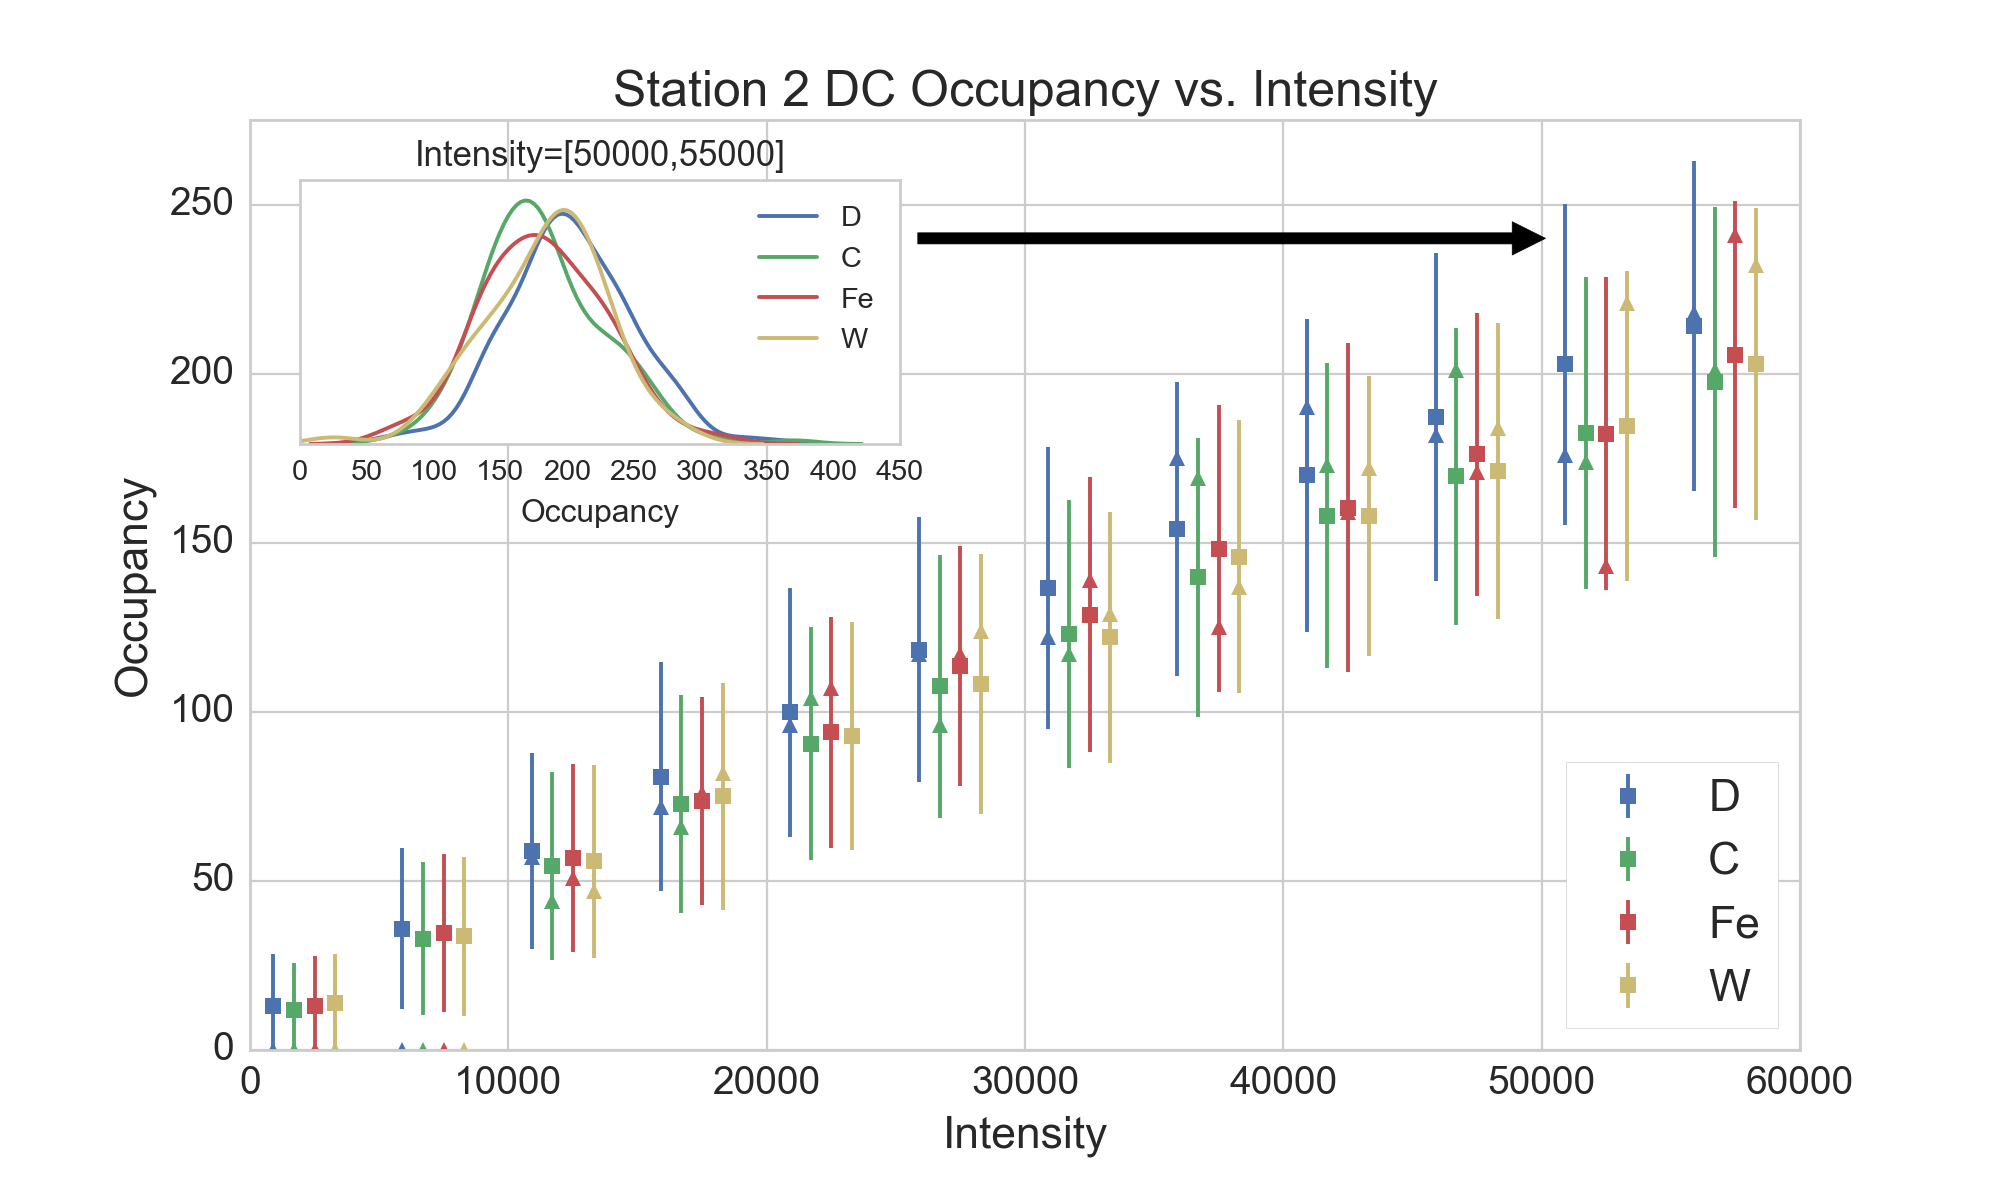
\includegraphics[width=5in]{figures/analysis/targ-occupancy.png}
	\caption{The Station 2 drift chamber occupancy for the four targets as a function of intensity. The error bars show a systematic deviation of occupancies from the mean for a given intensity bin. The inset plot shows a KDE plot of distributions for the intensity bin in which the values differ the most. The triangle markers represent the modes of the distributions.}
	\label{fig:occ-int-targ}
\end{figure}

To override any concern of chamber efficiencies having an effect on any absolute or ratio measurements, a study was performed to measure the effect of chamber efficiencies on the track reconstruction algorithm. This was done by embedding clean Monte Carlo-generated Drell-Yan dimuons into real NIM3 random event hit data. Then, a constant 94\% chamber efficiency was applied by removing a random 6\% of the chamber hits, and tracking was performed on this sample. The 94\% figure reflects the best estimate of overall chamber efficiencies at SeaQuest. Following that, a rate-dependent chamber efficiency was imposed of the form
\begin{equation}
\varepsilon(I) = 0.95 - a \cdot I
\end{equation}
where $a$ was set to \unit[2e-6]{protons$^{-1}$}. This resulted in a linear drop in efficiency with it dropping to as low as 75\% at the highest intensity regions considered (\unit[100000]{protons}). The tracking algorithm was then run on this data sample.
	
For even the constant 94\% efficiency case, the tracking is expected to decrease in \emph{tracking efficiency} (a very different topic to tackle, as we will approach later in this chapter) as intensity increases and pattern recognition becomes more difficult as overall occupancies increase. The important to observation to make is how this intensity-dependent tracking efficiency compares to the case of decreasing efficiency. For both cases, the ratio of successful reconstructions to all thrown dimuons (before even the trigger acceptance is imposed) can be seen in Figure~\ref{fig:ktrack-eff-int}. It is perhaps surprising to see that even at high intensities, the linear drop in tracking efficiencies does not change between the two cases. The reason for this is due to the fact that the tracking algorithm is very \emph{robust} in the way it is able to handle missing hits, as it only requires a few hits in each station (4 out of 6) to successfully find a track.
\begin{figure}
	\centering
	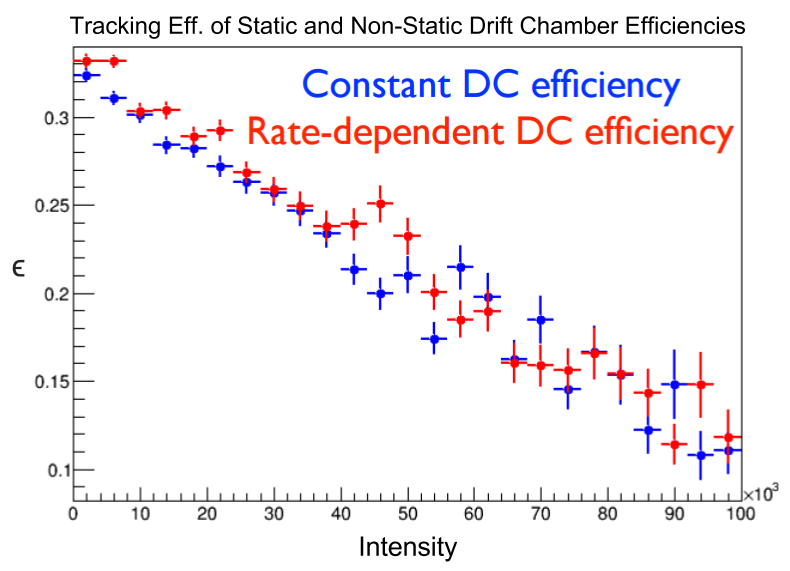
\includegraphics[width=4in]{figures/analysis/ktrack-eff-int.png}
	\caption{The ratio of successful reconstruction to all thrown by MC for two chamber efficiency models. The linear decreases in efficiency are not significantly different from each other.}
	\label{fig:ktrack-eff-int}
\end{figure}

Putting this together:
\begin{itemize}
	\item Differences in chamber efficiencies between targets could only arise from different chamber occupancies as a result of the varying targets.
	\item Chamber occupancies are only slightly different for deuterium when compared to the other nuclear targets.
	\item Even in the case of vastly different efficiencies, the yields from tracking remain unchanged.
	\item As a result, the effect of chamber efficiency on the yields will be the same for all targets.
	\item $\varepsilon^D/\varepsilon^A$, a measure of how the chamber efficiency effects the deuterium target yields as compared to a nuclear targets, can therefore be considered to be 1.
\end{itemize}

\subsection{Detector Acceptance}

The \emph{true} acceptance as a function of any set of kinematic variables $\bar{x}$ can be expressed as:
\begin{equation}
A(x) = \lim\limits_{N\rightarrow \infty} \frac{Y_{accepted}(\bar{x})}{Y_{thrown} (\bar{x})}\ \ ;\ \ 
N \equiv \int Y_{thrown}(\bar{x}) dx
\end{equation}
where \emph{thrown} denotes Drell-Yan simulated events from Monte Carlo which generates every kinematic value by sampling over the distributions of that variable with a random number generator. The simulation includes such processes as multiple scattering and energy loss that occur due to particle passage through materials (such as our targets and beam dumps). Survey numbers of the experimental hall are used to build an accurate representation of the apparatus and its sensitive detector regions. Muon pairs over much of the kinematic phase space and was weighted according to the known Drell-Yan cross section. This does not factor in any higher order nuclear effects or anything like $\dbar/\ubar$ asymmetries. 

The pairs that qualify as \emph{accepted} are those that satisfy the following two criteria: (1) were able to trace their way through the spectrometer without leaving the sensitive range of the detectors at all stations, and (2) they followed paths that would have satisfied the un-like-sign dimuon trigger (FPGA1). Such data was written to file in a format that matches real experimental data and is then ready for analysis. These events are weighted according to the kinematics and DY cross-section as mentioned above, but for analysis, these weights when analyzed were divided by $N$, the number of thrown events.

\begin{figure}
	\centering
	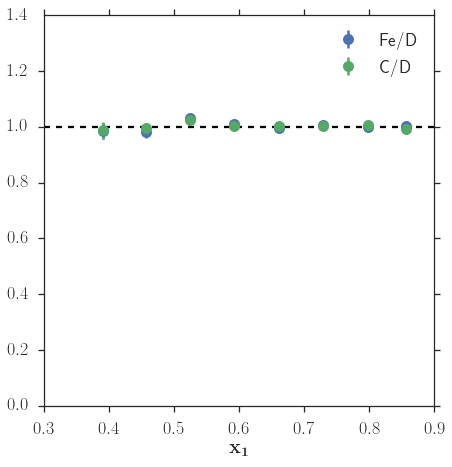
\includegraphics[height=0.3\textheight]{figures/analysis/x1-acceptance.png}\hfill
	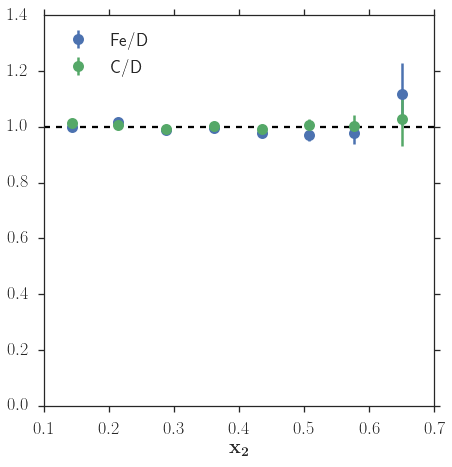
\includegraphics[height=0.3\textheight]{figures/analysis/x2-acceptance.png} \\
	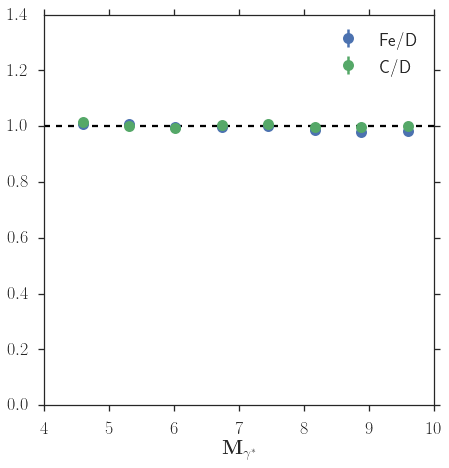
\includegraphics[height=0.3\textheight]{figures/analysis/mass-acceptance.png}\hfill
	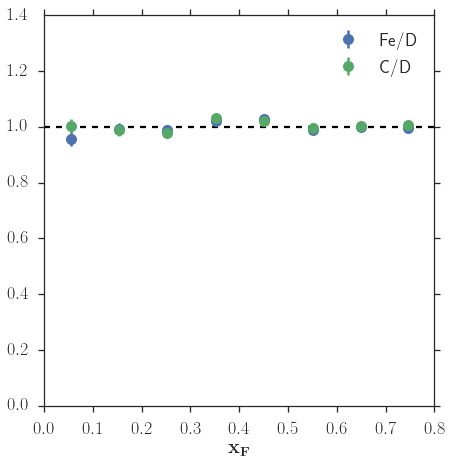
\includegraphics[height=0.3\textheight]{figures/analysis/xf-acceptance.png} \\
	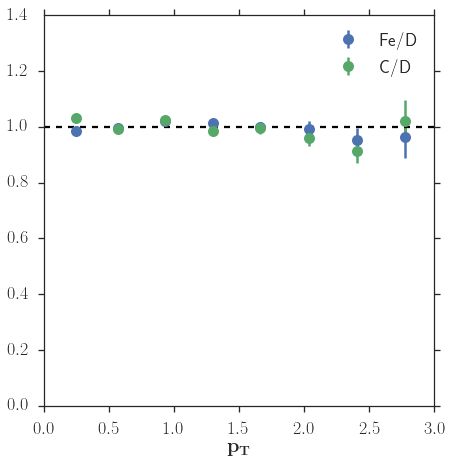
\includegraphics[height=0.3\textheight]{figures/analysis/pt-acceptance.png}
	\caption{Ratios of accepted dimuons from heavy targets to deuterium for all kinematic regions of interest.}
	\label{fig:targ-acceptance}
\end{figure}

Approximately \unit[800,000]{dimuons} were thrown for each target to have the acceptances analyzed. For an absolute acceptance, a study of a full $4\pi$ (or $2\pi$) simulation is required, where $4\pi$ is the solid angle of an entire (semi-)sphere. In such simulations dimuons are thrown in every physically possible direction, and then one can derive the absolute acceptance of the target and/or spectrometer when taking into account this source of \emph{thrown} events. However, for the purposes of these studies, we are only concerned about $\bar{\Omega}^D/\bar{\Omega}^A$, or the relative acceptance correction. As we see in Fig.~\ref{fig:table-layout}, we see that though the spatial distribution of the liquid deuterium flask and the solid targets are similar, they are fundamentally differently distributed. The density of the deuterium in the flask is constant throughout the length of the flask while the disks are discrete and separated. As a result, it perhaps may be the case that due to beam attenuation, there is a spatial difference between where most dimuons are generated between the different targets. The cause of any acceptance difference, however, is moot; the goal here is to estimate the relative acceptance correction factor between deuterium and the nuclear targets.

The target dependence of the acceptance was studied via yield ratios of heavy targets to that of deuterium for the valid kinematic regions of the experiment. These regions are \unit[4.2]{GeV}$<M_{\gamma^*}<$\unit[10]{GeV}, $0.1<x_2<0.58$, $0.35<x_1<0.85$, $0.0<x_F<0.8$, and \unit[0.0]{GeV}$<p_T<$\unit[2.5]{GeV}. Since no nuclear effects are simulated by the Monte Carlo generator, this ratio should lie at 1; any deviation of this must be purely from the acceptance effects due to the slight differences in the geometries and densities of the targets. The results can be seen in Figure~\ref{fig:targ-acceptance}.

In order to determine an acceptance correction, the ratio values shown are compared to the line of unity. The parameter $\alpha$ in the expression $1 - \alpha \cdot R_{DY}(k) = 0$ is optimized and is used as this correction factor in the target-to-target normalization. The acceptances of the liquid deuteriumt is found to be $\alpha = 0.9989 \pm 0.0012$ smaller than that of the solid targets. As such, a correction factor of $$\bar{\Omega}^D/\bar{\Omega}^A = 0.9989$$ is included in the target-to-target normalization. The systematic uncertainty of this correction is approximately 0.1\%.

\section{Rate Dependence}

\begin{figure}
	\centering
	\begin{minipage}{0.48\textwidth}
		\centering
		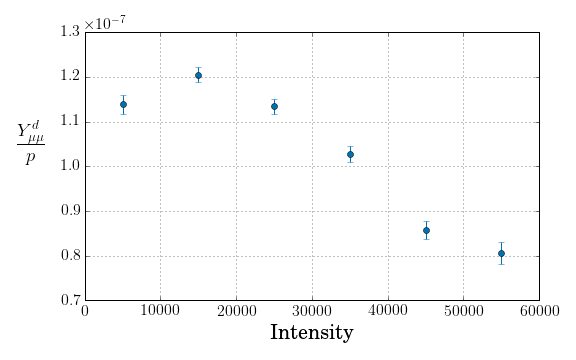
\includegraphics[width=\textwidth]{figures/analysis/rate-dep.png}
		\caption{The rate dependence, depicting the decline in yields per triggering proton as a function of the overall environmental chamber intensity.}
		\label{fig:ratedep}
	\end{minipage}\hfill
	\begin{minipage}{0.48\textwidth}
		\centering
		\includegraphics[width=\textwidth]{figures/analysis/rate-dep-x2.png}
		\caption{The rate dependence has a different behavior for different kinematics. Shown is the same plot as in Fig.~\ref{fig:ratedep}, but in three statistically equal $x_2$ bins.}
		\label{fig:x2-ratedep}
	\end{minipage}
\end{figure}

From the many generations of high energy experiments preceeding SeaQuest, it was known that there might be an issue of \emph{Rate Dependence} in the results of the data. This happens when conditions that lead to good reconstruction of signal events are affected by intensity or fluctuations in intensity of the beam delivered to the experiment. This was the case with E-772~\cite{Wang:1991wa} and E-866~\cite{Towell:2001nh}, and so given the highly erratic nature of the beam from the slow spill extraction, such an effect was anticipated at SeaQuest.

It was uncovered in early 2015 that SeaQuest indeed had a rate dependence problem as well. This was done by investigating the number of reconstructed dimuons per trigger proton and plotting those yields against the chamber intensity (Figure~\ref{fig:ratedep}). Here, we define the terms \textbf{trigger intensity} as referring to the number of protons in the RF bucket that triggered the event, and \textbf{chamber intensity} as a weighted sum of the number of protons $\pm$13 RF buckets about the triggerred RF bucket. The former gives a measure of the number of protons on which the trigger could have fired while the latter gives a measure to the general intensity \emph{environment} of the triggerred event. It was observed that as the chamber intensity increases, the yields per trigger proton would drop precipitously, where the value is desired to remain stable at any intensity. The goal in this section is to apply a series of corrections to bring these plots show a flat series of values vs. chamber intensity.

To complicate the matter further, the rate dependence has a kinematic-dependence -- or perhaps it is more accurate to say that the rate dependence affects some signal events with certain kinematics more severely than others. The kinematic dependence can be seen by simply showing the plot from Figure~\ref{fig:ratedep}, but with the data split up into a few bins. The $x_2$ dependendence of the rate dependence can be seen by observing the shape of the distributions in Figure~\ref{fig:x2-ratedep}. What this implies is that a single intensity-dependent correction factor (as used in the two aforementione experiments) would be inappropriate for correcting the data, and thus the correction becomes rather complicated.

The issue of rate dependence is discussed here, and as the sources of this effect are identified, a correction is proposed, calculated, and applied for each source in the form of an event weight. The two known sources addressed in this paper are the reconstruction efficiencies and empty target background corrections.

\subsection{Weights as Corrections}

Weighting of events is a standard procedure for mapping one distribution onto another. The most common example is with Monte Carlo (MC) simulation weighting. A simple physics event MC meant to simulate a well-defined process will `throw' an event with certain kinematics randomly drawn from known distributions via \emph{inverse transform sampling}. By doing this, the simulation is already close to being physical, but according to the cross section of a given process, a certain combination of kinematics will be decidedly more or less probable. A weighting subroutine calculates this likelihood for each event and assigns a weight with respect to how likely that event is based on the kinematics thrown. When binning this weighted data, the adjusted number of events in a bin is given by
\begin{equation}
	N_{bin} = \sum_{i \in bin} w_i\ \ ;\ \ \sigma_{bin} = \sqrt{\sum_{i\in bin} w_i^2}
	\label{eq:gmc-weight}
\end{equation}
which reduces to the Poissonian statistical picture when all weights are 1.

Weighting in this manner can be used in any case where it is desirable to map one distribution to another, as in the case of applying the corrections discussed in this section. The most intuitive connection between the use of weights and corrections is in the case of efficiency corrections. Let us say that a dimuon with a certain set of kinematics, for whatever combination of effects, has a reconstruction efficiency of 80\%. This means that four out of five actual dimuons with these kinematics will be reconstructed. If you know this efficiency $\epsilon$, you can apply a weight as $w = 1/\epsilon_{recon}$ to each dimuon, as each observed event represents, in part, a larger population that is not fully represented. In the case of our example, a single dimuon represents $1/0.80 = 1.25$ dimuons in order to make up for the ones that are missed due to that specific inefficiency, and so this weight would be applied to the event.

\subsection{Tracking Efficiency}\label{sec:keff}

As the intensity increases, the number of background hits on all of the detectors increases. As the number of hits in all the detectors increases, the harder it become for the tracking to perform its pattern recognition to discern the actual dimuon(s) from the whole event. This is regarded to be an intensity-dependent tracking efficiency. Seeing as the primary tracking algorithm for SeaQuest is kTracker, this referred to at SeaQuest as the \textbf{``kEfficiency''}. Its intensity, target, and kinematic dependence makes it a factor to model and correct for.

The procedure developed by Evan McClellan of UIUC for calculating this kEfficiency is to compare the performance of the tracking on a clean MC sample of dimuons to an analogous sample that's mixed in with real intensity-dependent background. To do this, a \emph{single} sample of MC-generated dimuons and all of their hits is generated; this sample is denoted as the \emph{``clean''} sample. Then, this \emph{same} sample is mixed with all of the hits from a NIM3 event from the experimental data. The NIM3 trigger, as is discussed in Chapter~2, is the ``random'' trigger, and by using these events we avoid any effects due to trigger selection bias. This mix of MC dimuons and NIM3 triggered data is denoted as the \emph{``messy''} sample. These NIM3 events all have an intensity, and by embedding a clean MC dimuon into a situation typical of an event at a given intensity, we get a basis by which to judge how efficiently the tracking can reconstruct a dimuon in the clean sample versus the messy sample as a function of intensity (and other kinematic variable).

It is important to note that the DY cross section is so small that there is a negligible chance that a given randomly-triggered NIM3 event will contain an actual dimuon, nonetheless a dimuon matching the characteristics of the embedded MC dimuon. As such, it is assumed that the dimuon embedded in the NIM3 event is the only dimuon to find in the event. It is also justified to assume that the kinematics of a dimuon is in no way correlated to the intensity, and the intensity of an event relates only to the amount of background hits observed. The relation to the intensity and the number of background hits can be observed in Figure~\ref{fig:NIM3-Int-Mult}.

\begin{figure}
	\centering
	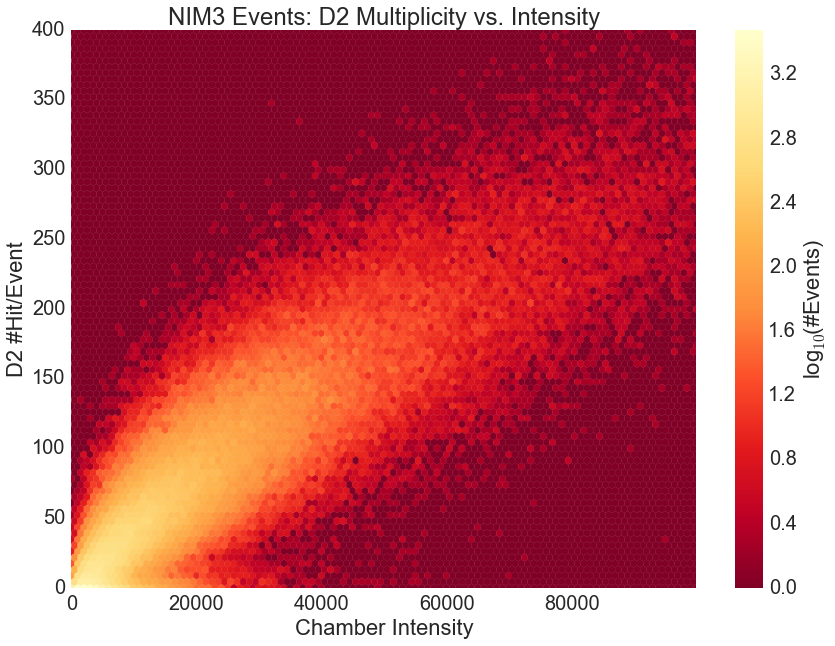
\includegraphics[width=4in]{figures/analysis/NIM3-Int-Mult.png}
	\caption{The linear tendency of detector multiplicity to increase with intensity is observed by looking to unbiased NIM3 events. Here, the occupancy per event of the drift chambers at station 2 are shown as a function of intensity.}
	\label{fig:NIM3-Int-Mult}
\end{figure}

The tracking software is run both clean and messy samples, and the two outputs are compared. The first step is to bin the resulting reconstructed dimuons into intensity bins. This binning uses the weights of the dimuons that is assigned by the GMC that created them. The weights are used instead to avoid undue influence on the efficiency from dimuons that are highly unlikely to occur. The value of the bin and its uncertainty are calculated according to Eq.~\ref{eq:gmc-weight}.

For each matching bin, the ratio of $\frac{\#messy}{\#clean}$ values is used to calculate the efficiency of the tracking for that bin. The uncertainty of that efficiency is more complicated, as the relation between the messy and clean samples is of a \emph{binomial} nature. Each dimuon successfully reconstructed in the messy sample represents a \emph{positive} outcome from the number of possible outcomes which is represented by the clean sample. With this kind of relationship, binomial uncertainty calculations must apply. For large enough N number of trials and efficiency $\epsilon\notin \{0,1\}$,
\begin{equation}
\epsilon = \frac{N_+}{N}\ \ ;\ \ \delta\epsilon = \sqrt{\frac{N_+ N_-}{N^3}} = \sqrt{\frac{\epsilon(1-\epsilon)}{N}}
\label{eq:binomial-naive}
\end{equation}
but when weighted trials are involved, things become more complicated in calculating the statistical error. The calculation of this statistical error~\cite{blist:binomial} is as follows:
\begin{eqnarray}
	\epsilon & = & \frac{\sum\limits_{i\in+}w_i}{\sum\limits_i w_i} \\
	\delta\epsilon & = & \frac{\sqrt{\sum\limits_{i\in+} w_i^2 \left(\sum\limits_{i\in-} w_i \right)^2 + \
			\sum\limits_{i\in-} w_i^2 \left(\sum\limits_{i\in+} w_i \right)^2}} {\left(\sum\limits_{i}w_i\right)^2}
	\label{eq:binomial-weighted}
\end{eqnarray}
where the sum of the weights (and sum of squares of the weights) for non-positive samples is approximated as
\begin{eqnarray}
\sum\limits_{i\in-} w_i & = & \sum\limits_{i}w_i - \sum\limits_{i\in+}w_i \\
\sum\limits_{i\in-} w_i^2 & = & \sum\limits_{i}w_i^2 - \sum\limits_{i\in+}w_i^2 .
\end{eqnarray}

For a set of efficiencies, an exponential function is fit to the efficiencies. This fit function would then be used to calculate the efficiency for any given dimuon that occurs at any given intensity. The single-parameter exponential function, $$f(x)=e^{-Ax},$$ is chosen for its behavior at zero and infinity. The function of best fit along with a confidence interval for this can be seen in Figure~\ref{fig:keff-all}.

\begin{figure}
	\centering
	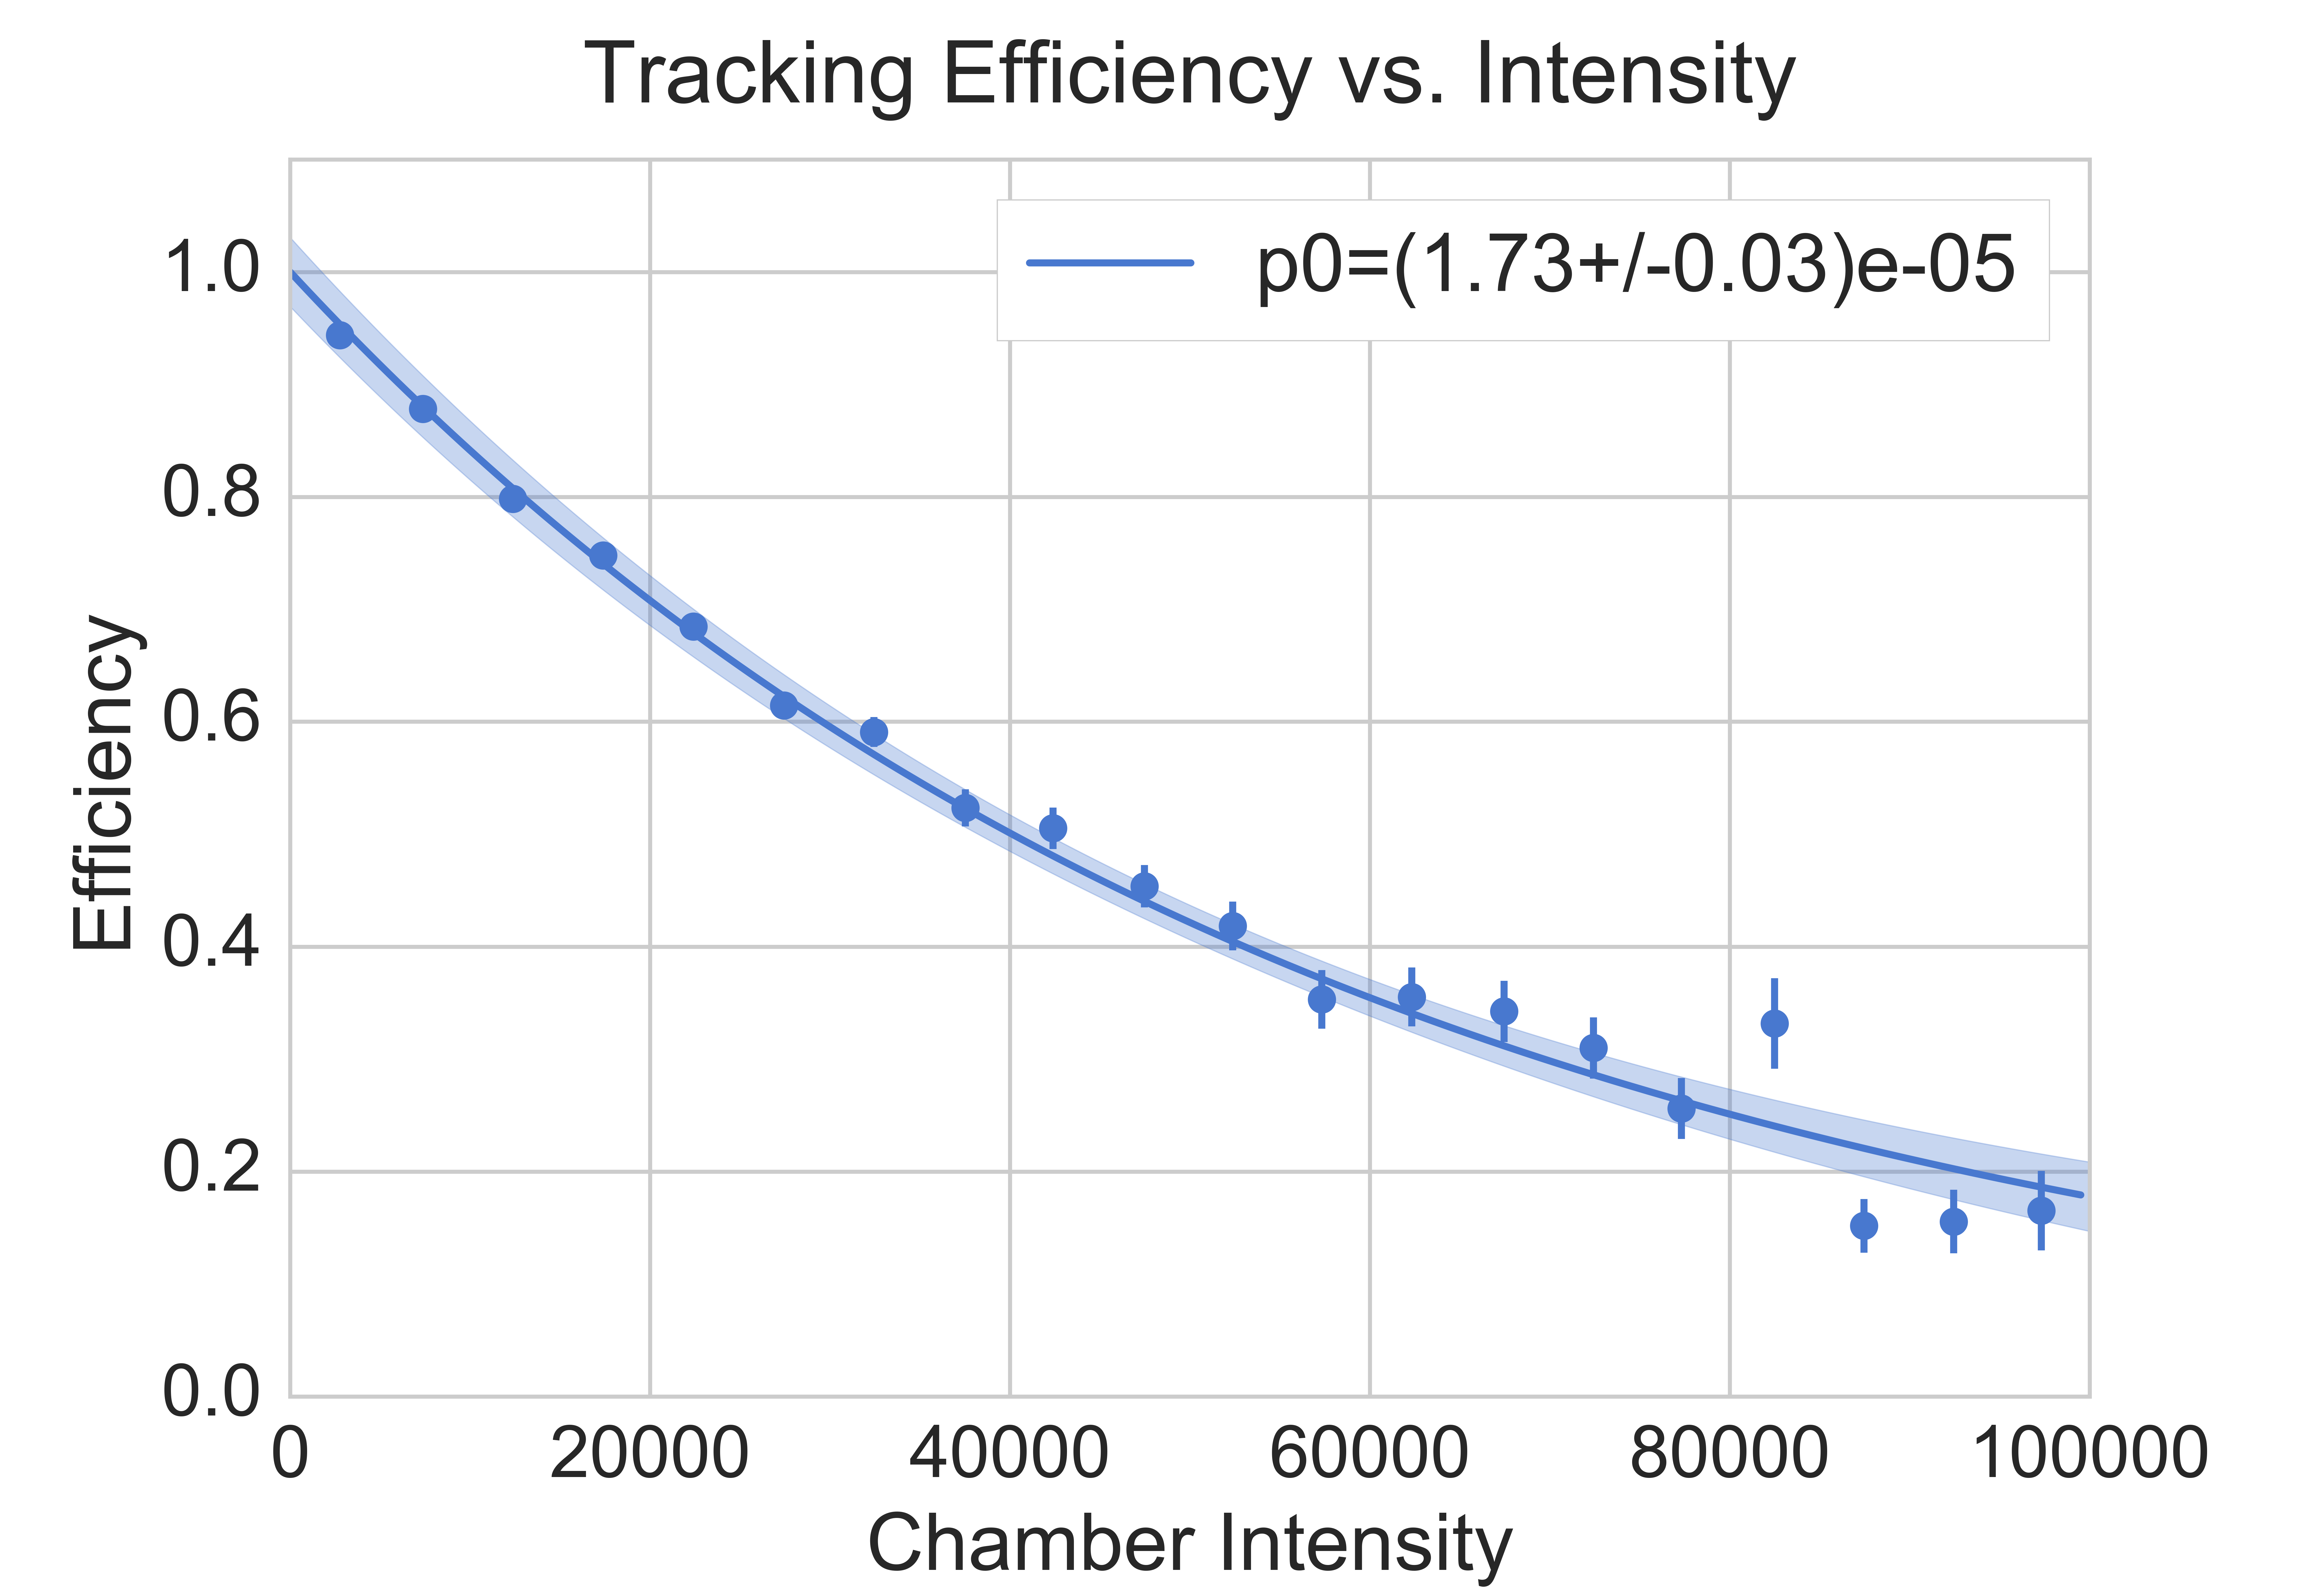
\includegraphics[width=4in]{figures/analysis/all-keff-int.png}
	\caption{The ratio of ``messy'' to ``clean'' dimuon samples from the Deuterium target in Roadset 67 data. This shows the linear relationship of the tracking efficiency to the intensity of the events. The shaded band indicates the 95\% confidence band of the fit.}
	\label{fig:keff-all}
\end{figure}

Further, these fits have a statistically significant kinematic dependence, so it becomes important to unfold the kinematic space and perform this procedure for several kinematic bins in one or more dimensions to assure a robust efficiency calculation. Of the six defining kinematics of the dimuon, we examine the dependence of the fit on five of them: ($x_1, x_2, p_T, \theta, \phi$), neglecting the azimuthal production angle $\phi_{\gamma^*}$. Each of these five kinematics is divided into three statistically equal bins (low, medium, high) in order to observe the efficiency dependencies. The results are shown in Figure~\ref{fig:keff-all-kin}.
\begin{figure}
\centering
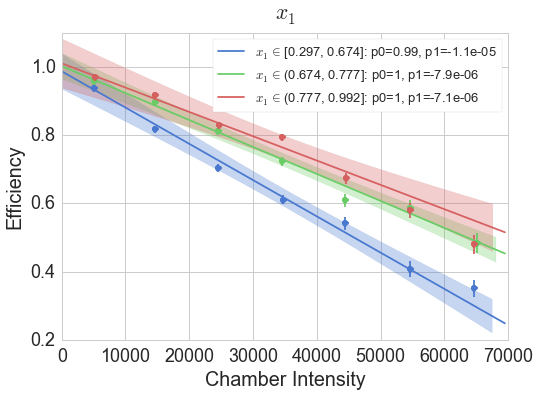
\includegraphics[width=0.49\textwidth]{figures/analysis/x1-keff-int.png}
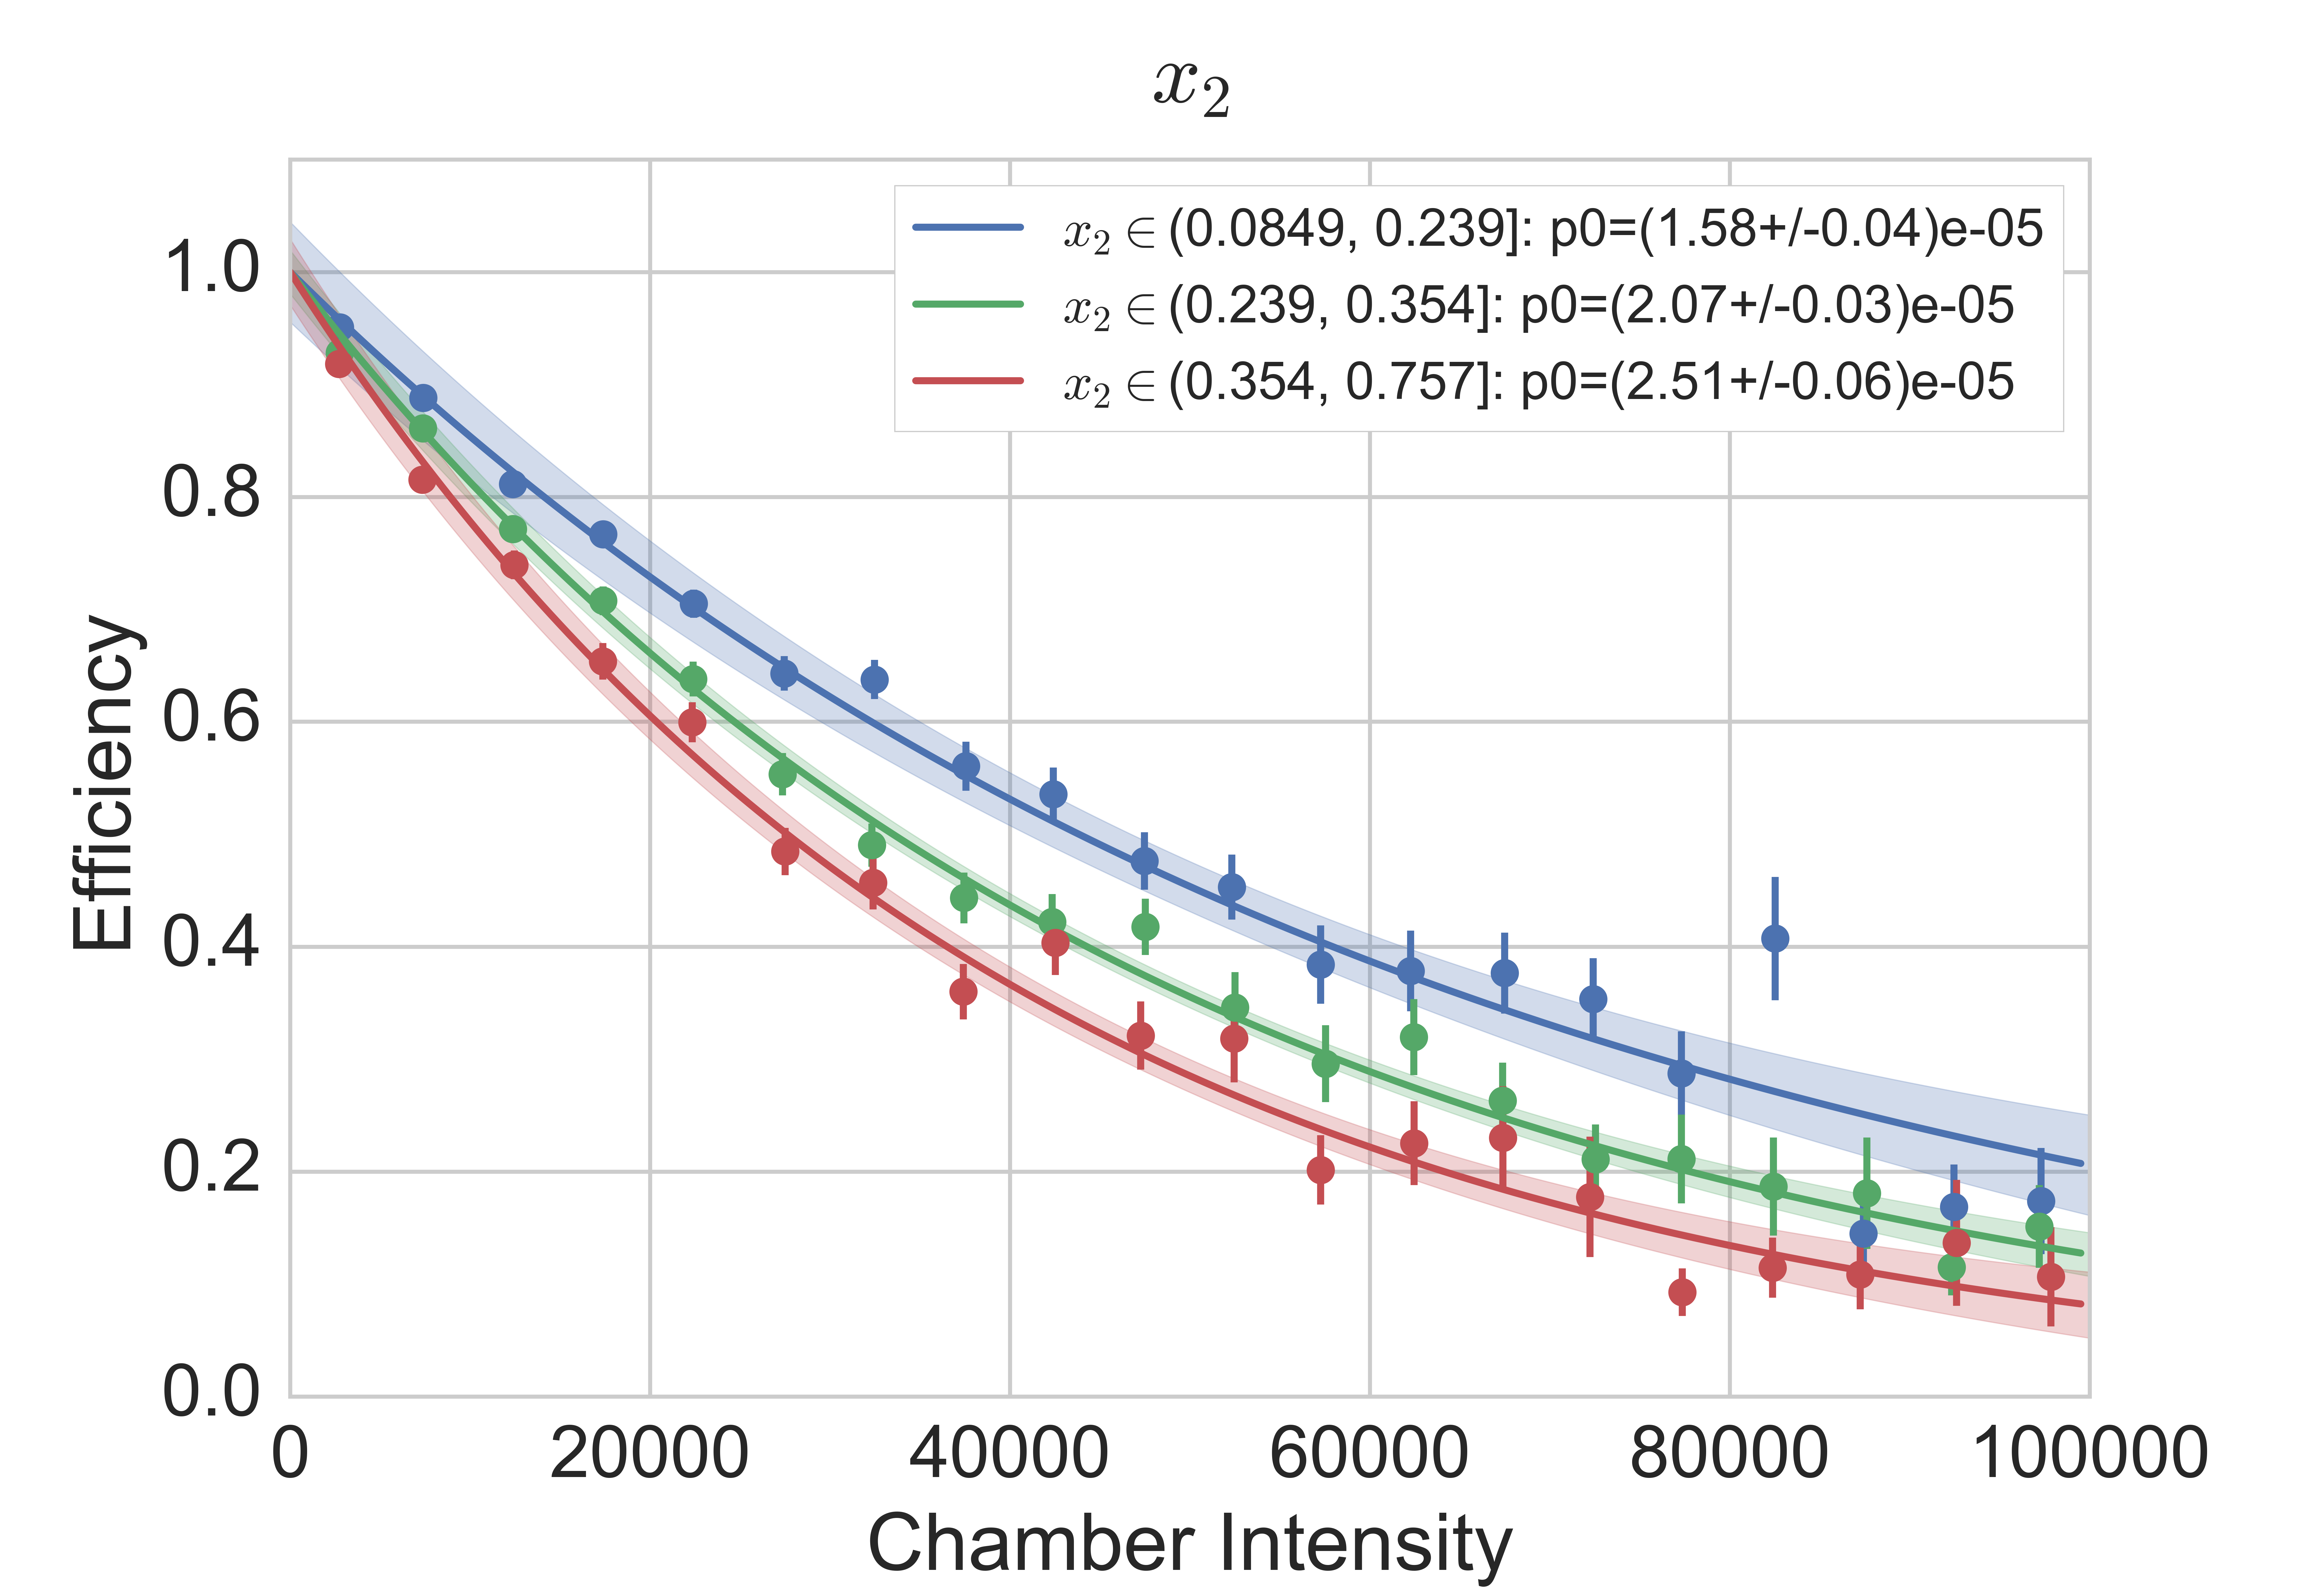
\includegraphics[width=0.49\textwidth]{figures/analysis/x2-keff-int.png} \\ \vspace{20px}
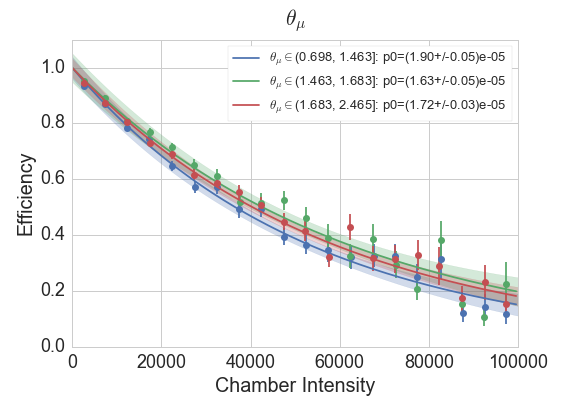
\includegraphics[width=0.49\textwidth]{figures/analysis/theta-keff-int.png}
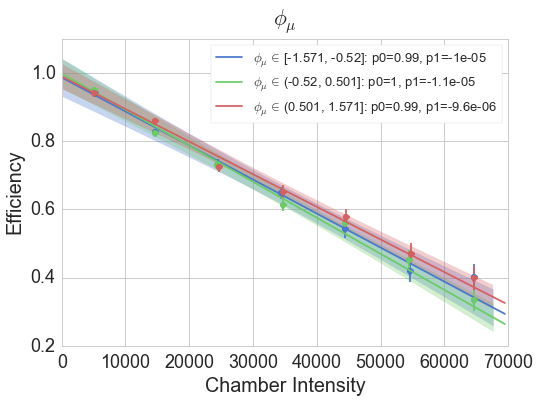
\includegraphics[width=0.49\textwidth]{figures/analysis/phi-keff-int.png} \\ \vspace{20px}
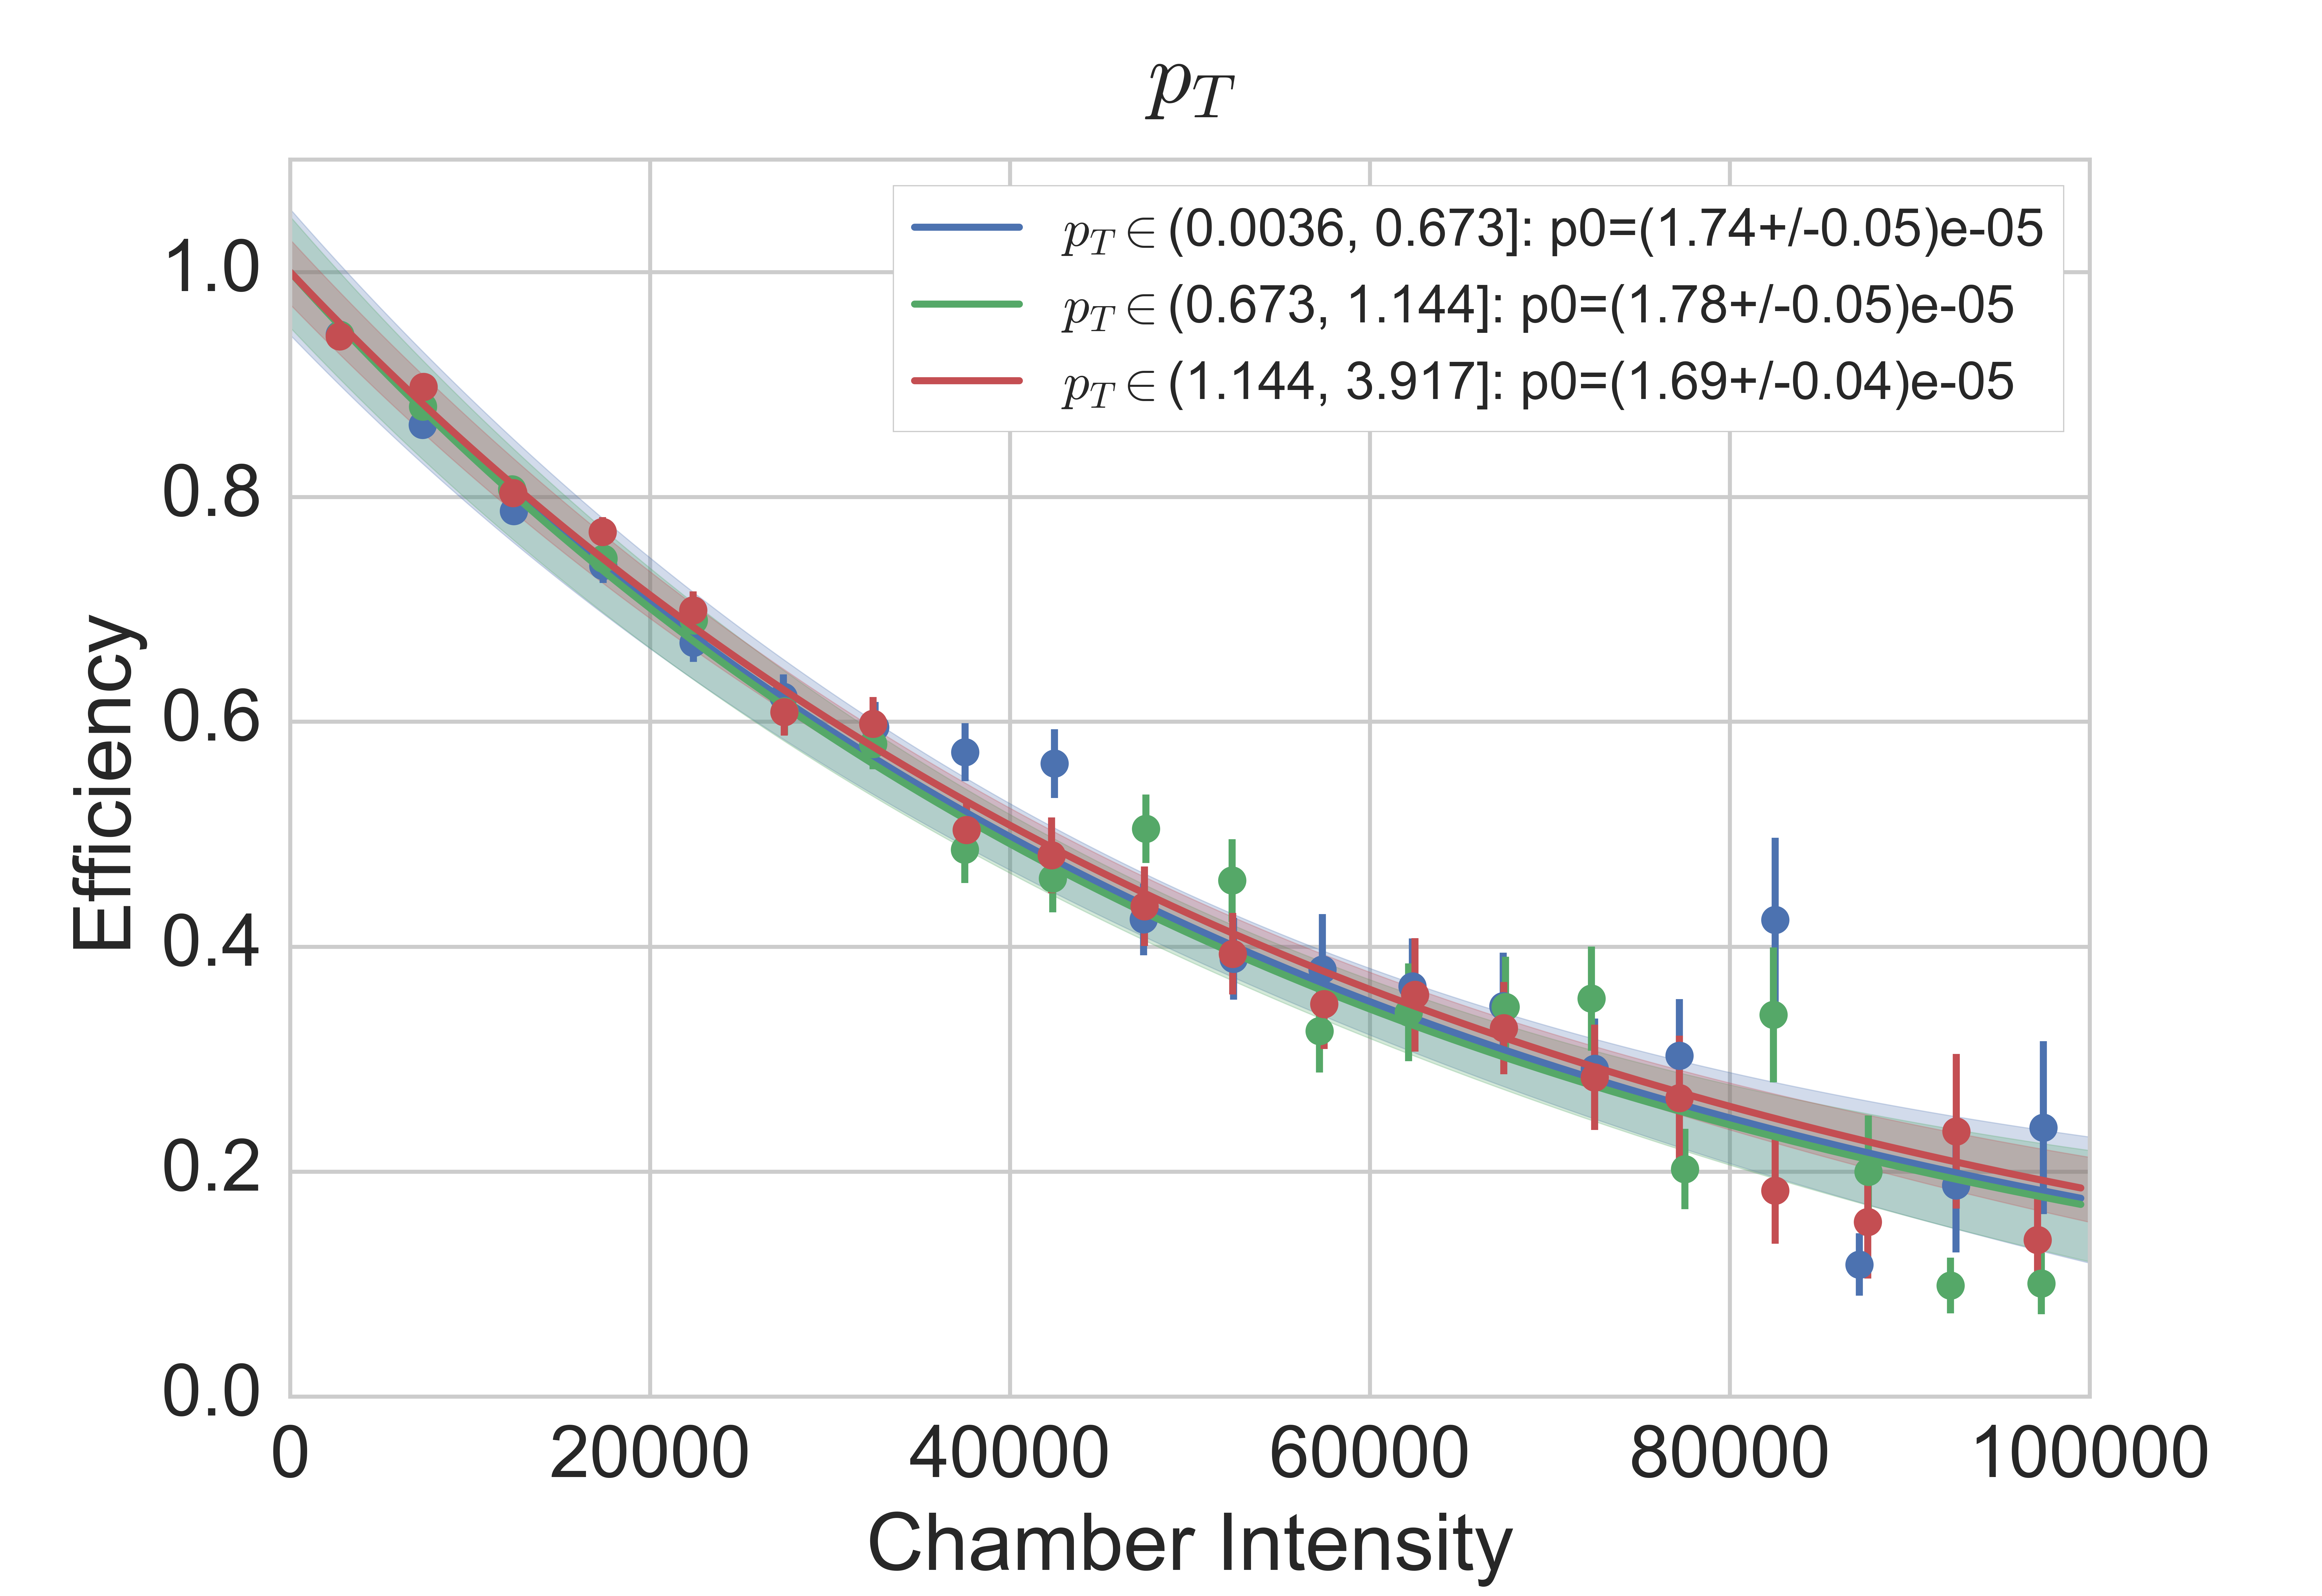
\includegraphics[width=0.49\textwidth]{figures/analysis/pt-keff-int.png} \vspace{10px}
\caption{Tracking efficiency with the data broken into three statistically equivalent bins in the five primary kinematics, ($x_1, x_2, \theta_\mu, \phi_\mu, p_T$). Significant kinematic dependence is seen in $x_1$ and $x_2$.}
\label{fig:keff-all-kin}
\end{figure}
The curves produced seem to indicate that there only exists a strong kinematic dependence on the $x_1$ and $x_2$ kinematics. If this is the case, then the clean and messy samples can be split two-dimensionally in these two kinematics, and a fit can be made to both variables. When analyzing dimuons, its kinematics can indicate which fit to use to calculate the tracking efficiency based on the intensity of the event, and a weight can be calculated.

But before we come to any clear conclusions, let us investigate two more kinematic phase spaces. We know from the discussion in Chapter 1 that \{$x_1, x_2$\} can be used almost interchangeably with \{$x_F, M_{\gamma^*}$\} to describe the same process. As such, it's possible that if only one and not the other shows to influence the tracking efficiency curves, then only that one might be needed for the tracking efficiency correction. We see the behavior of the efficiency curves as a function of $x_F$ and $M_{\gamma^*}$ in Figure~\ref{fig:keff-mass-xf}. It can be concluded that since there is no substantial mass dependence observed, the tracking efficiency has a kinematic dependence may be corrected by solely correcting on $x_F$.

\begin{figure}
	\centering
	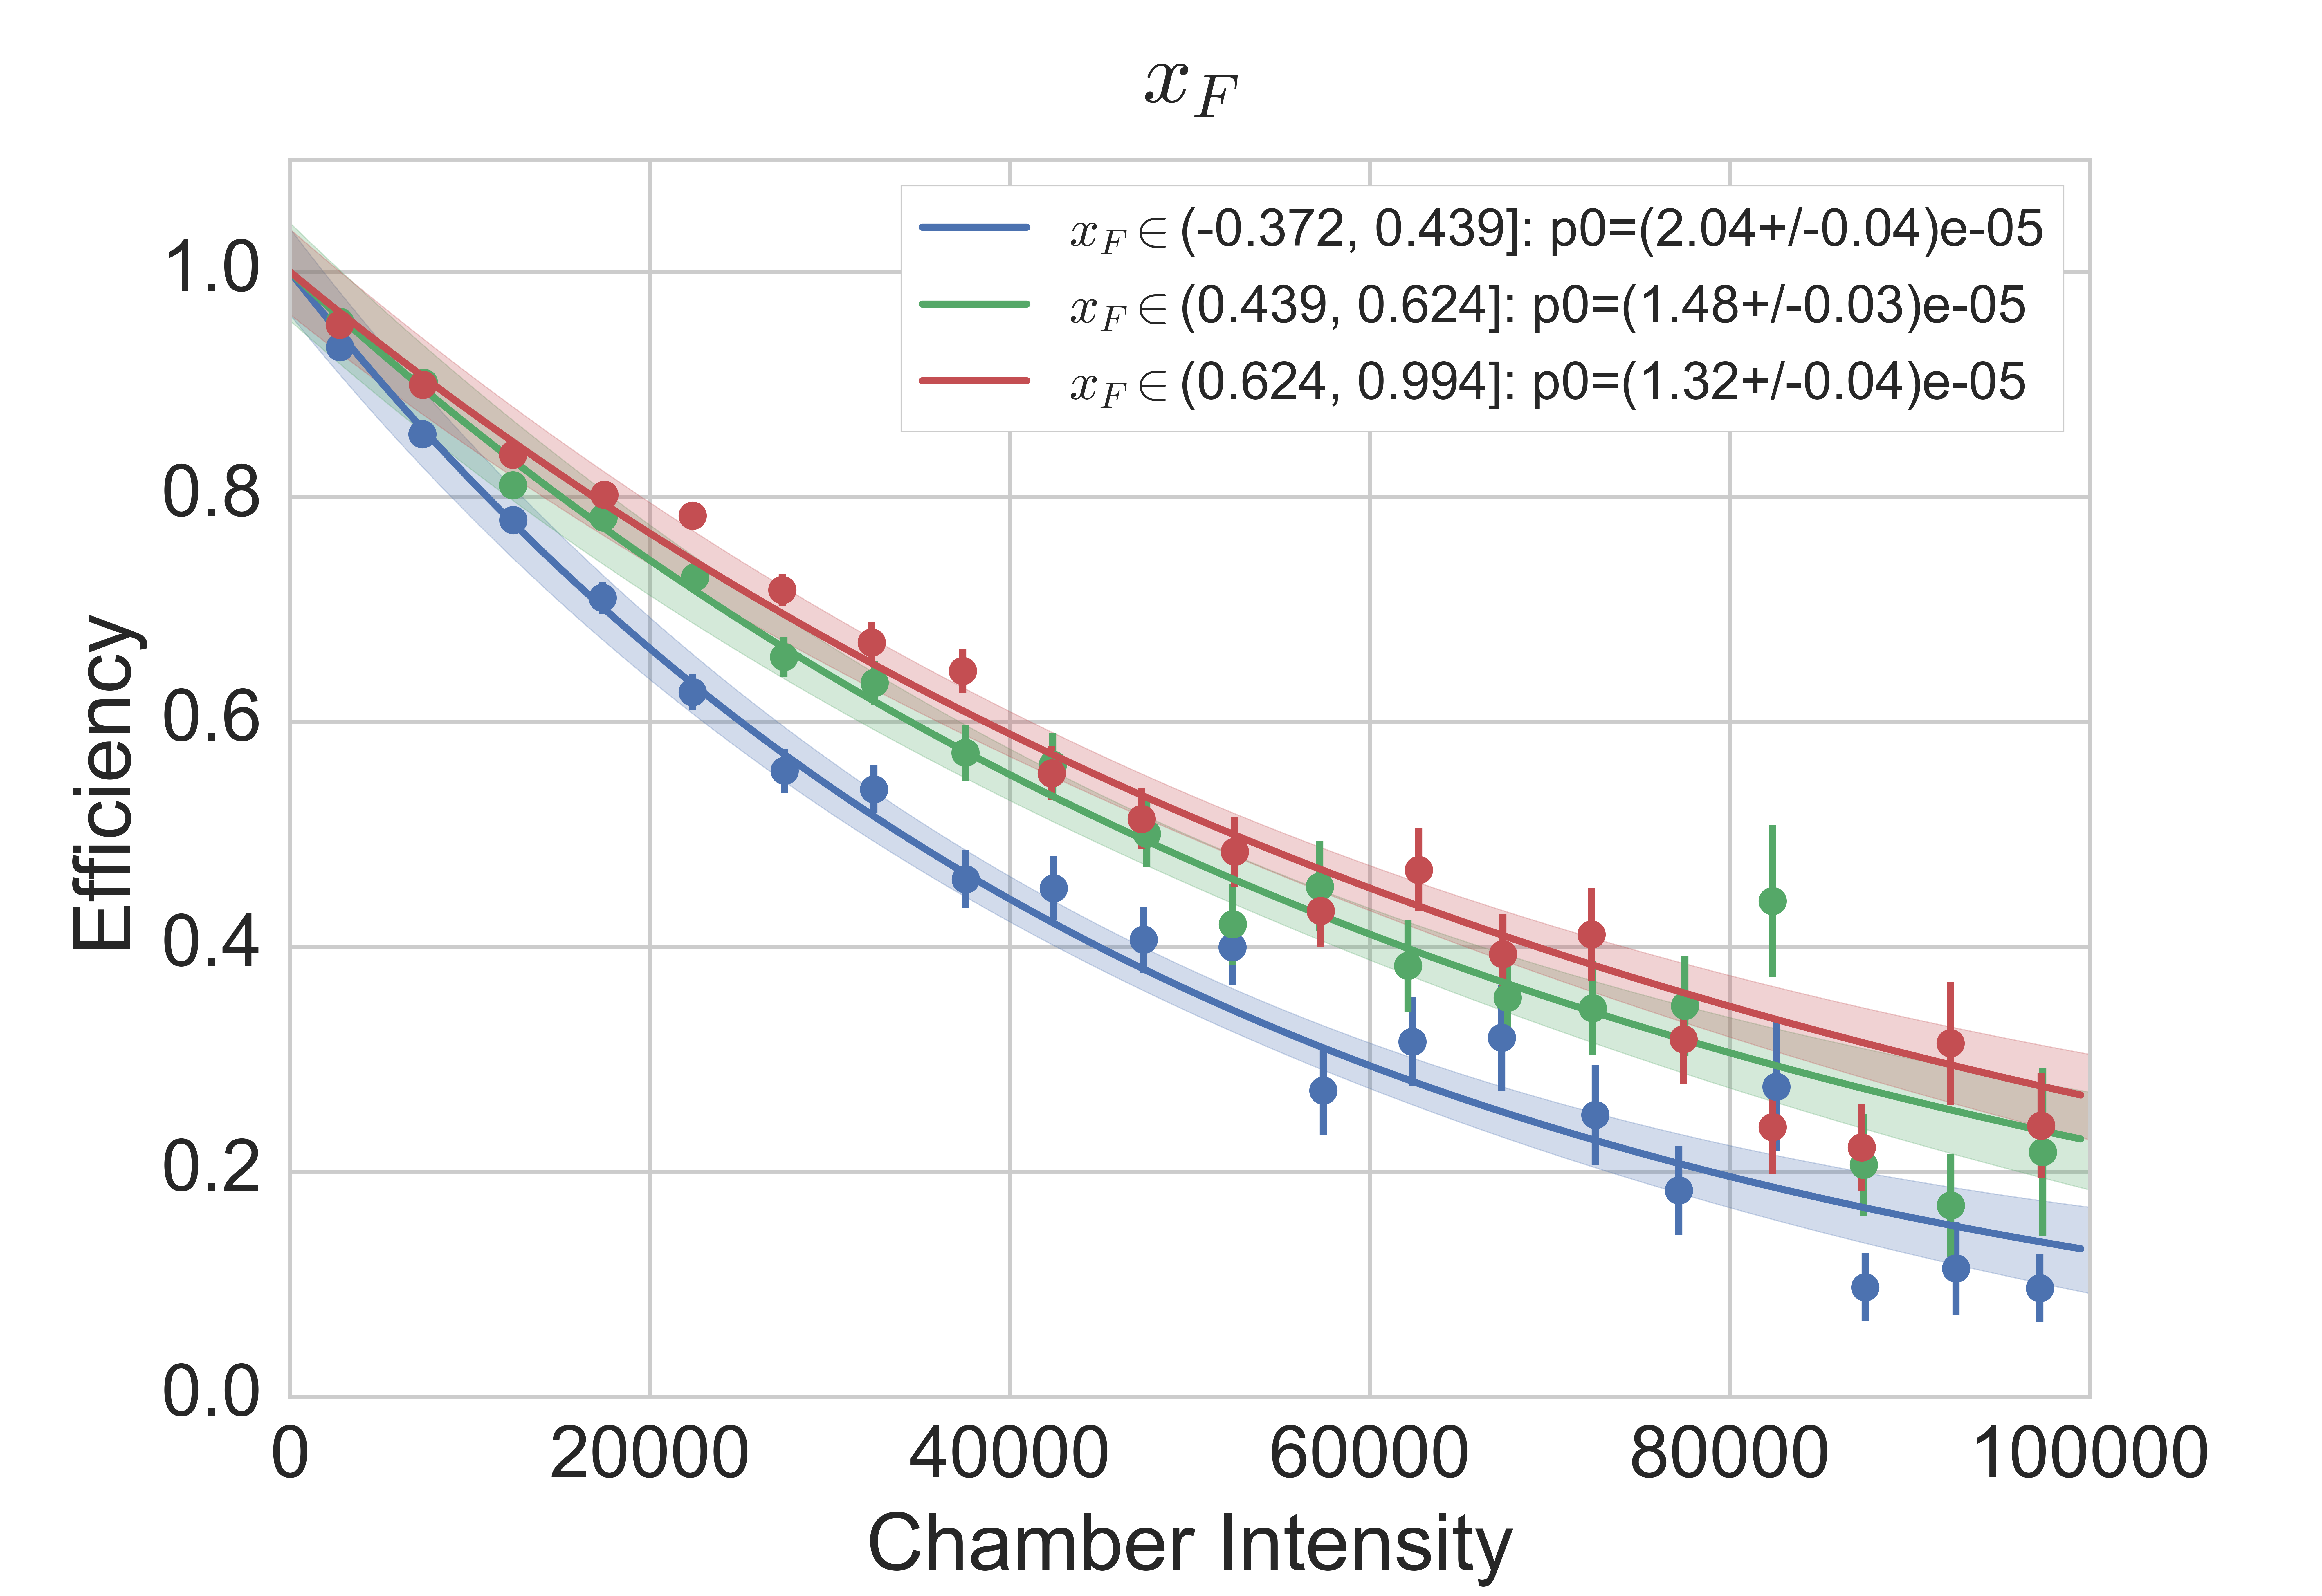
\includegraphics[width=0.49\textwidth]{figures/analysis/xF-keff-int.png}
	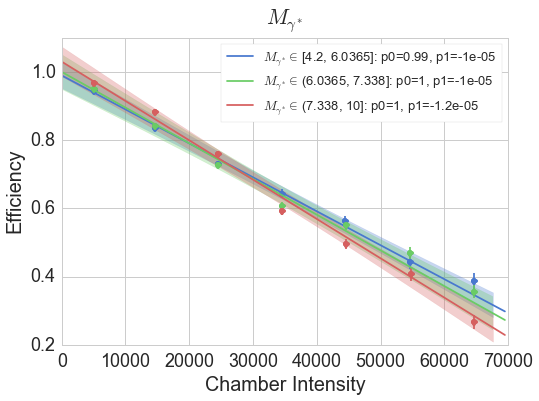
\includegraphics[width=0.49\textwidth]{figures/analysis/mass-keff-int.png}
	\caption{The kinematics $x_F$ and $M_{\gamma^*}$ are investigated. A clear kinematic dependence exists in $x_F$ while $M_{\gamma^*}$ is largely consistent.}
	\label{fig:keff-mass-xf}
\end{figure}

In order to evaluate the effectiveness of a correction, the messy sample was reweighted with the kEfficiency factors, with the efficiencies calculated in bins of $x_F$, and then recalculate these efficiency plots. This is shown in Figure~\ref{fig:xf-keff-corrected} for $x_F$ and also $x_2$ to see if by correcting in one, the other is also corrected. It becomes evident that even though the efficiency certainly seems to be fixed in $x_F$, any analysis in $x_2$ may not be properly corrected. One can come to the conclusion from this that \emph{if one performs an analysis on SeaQuest data in certain kinematics, one must correct for kEfficiency based on those kinematics}.
\begin{figure}
	\centering
	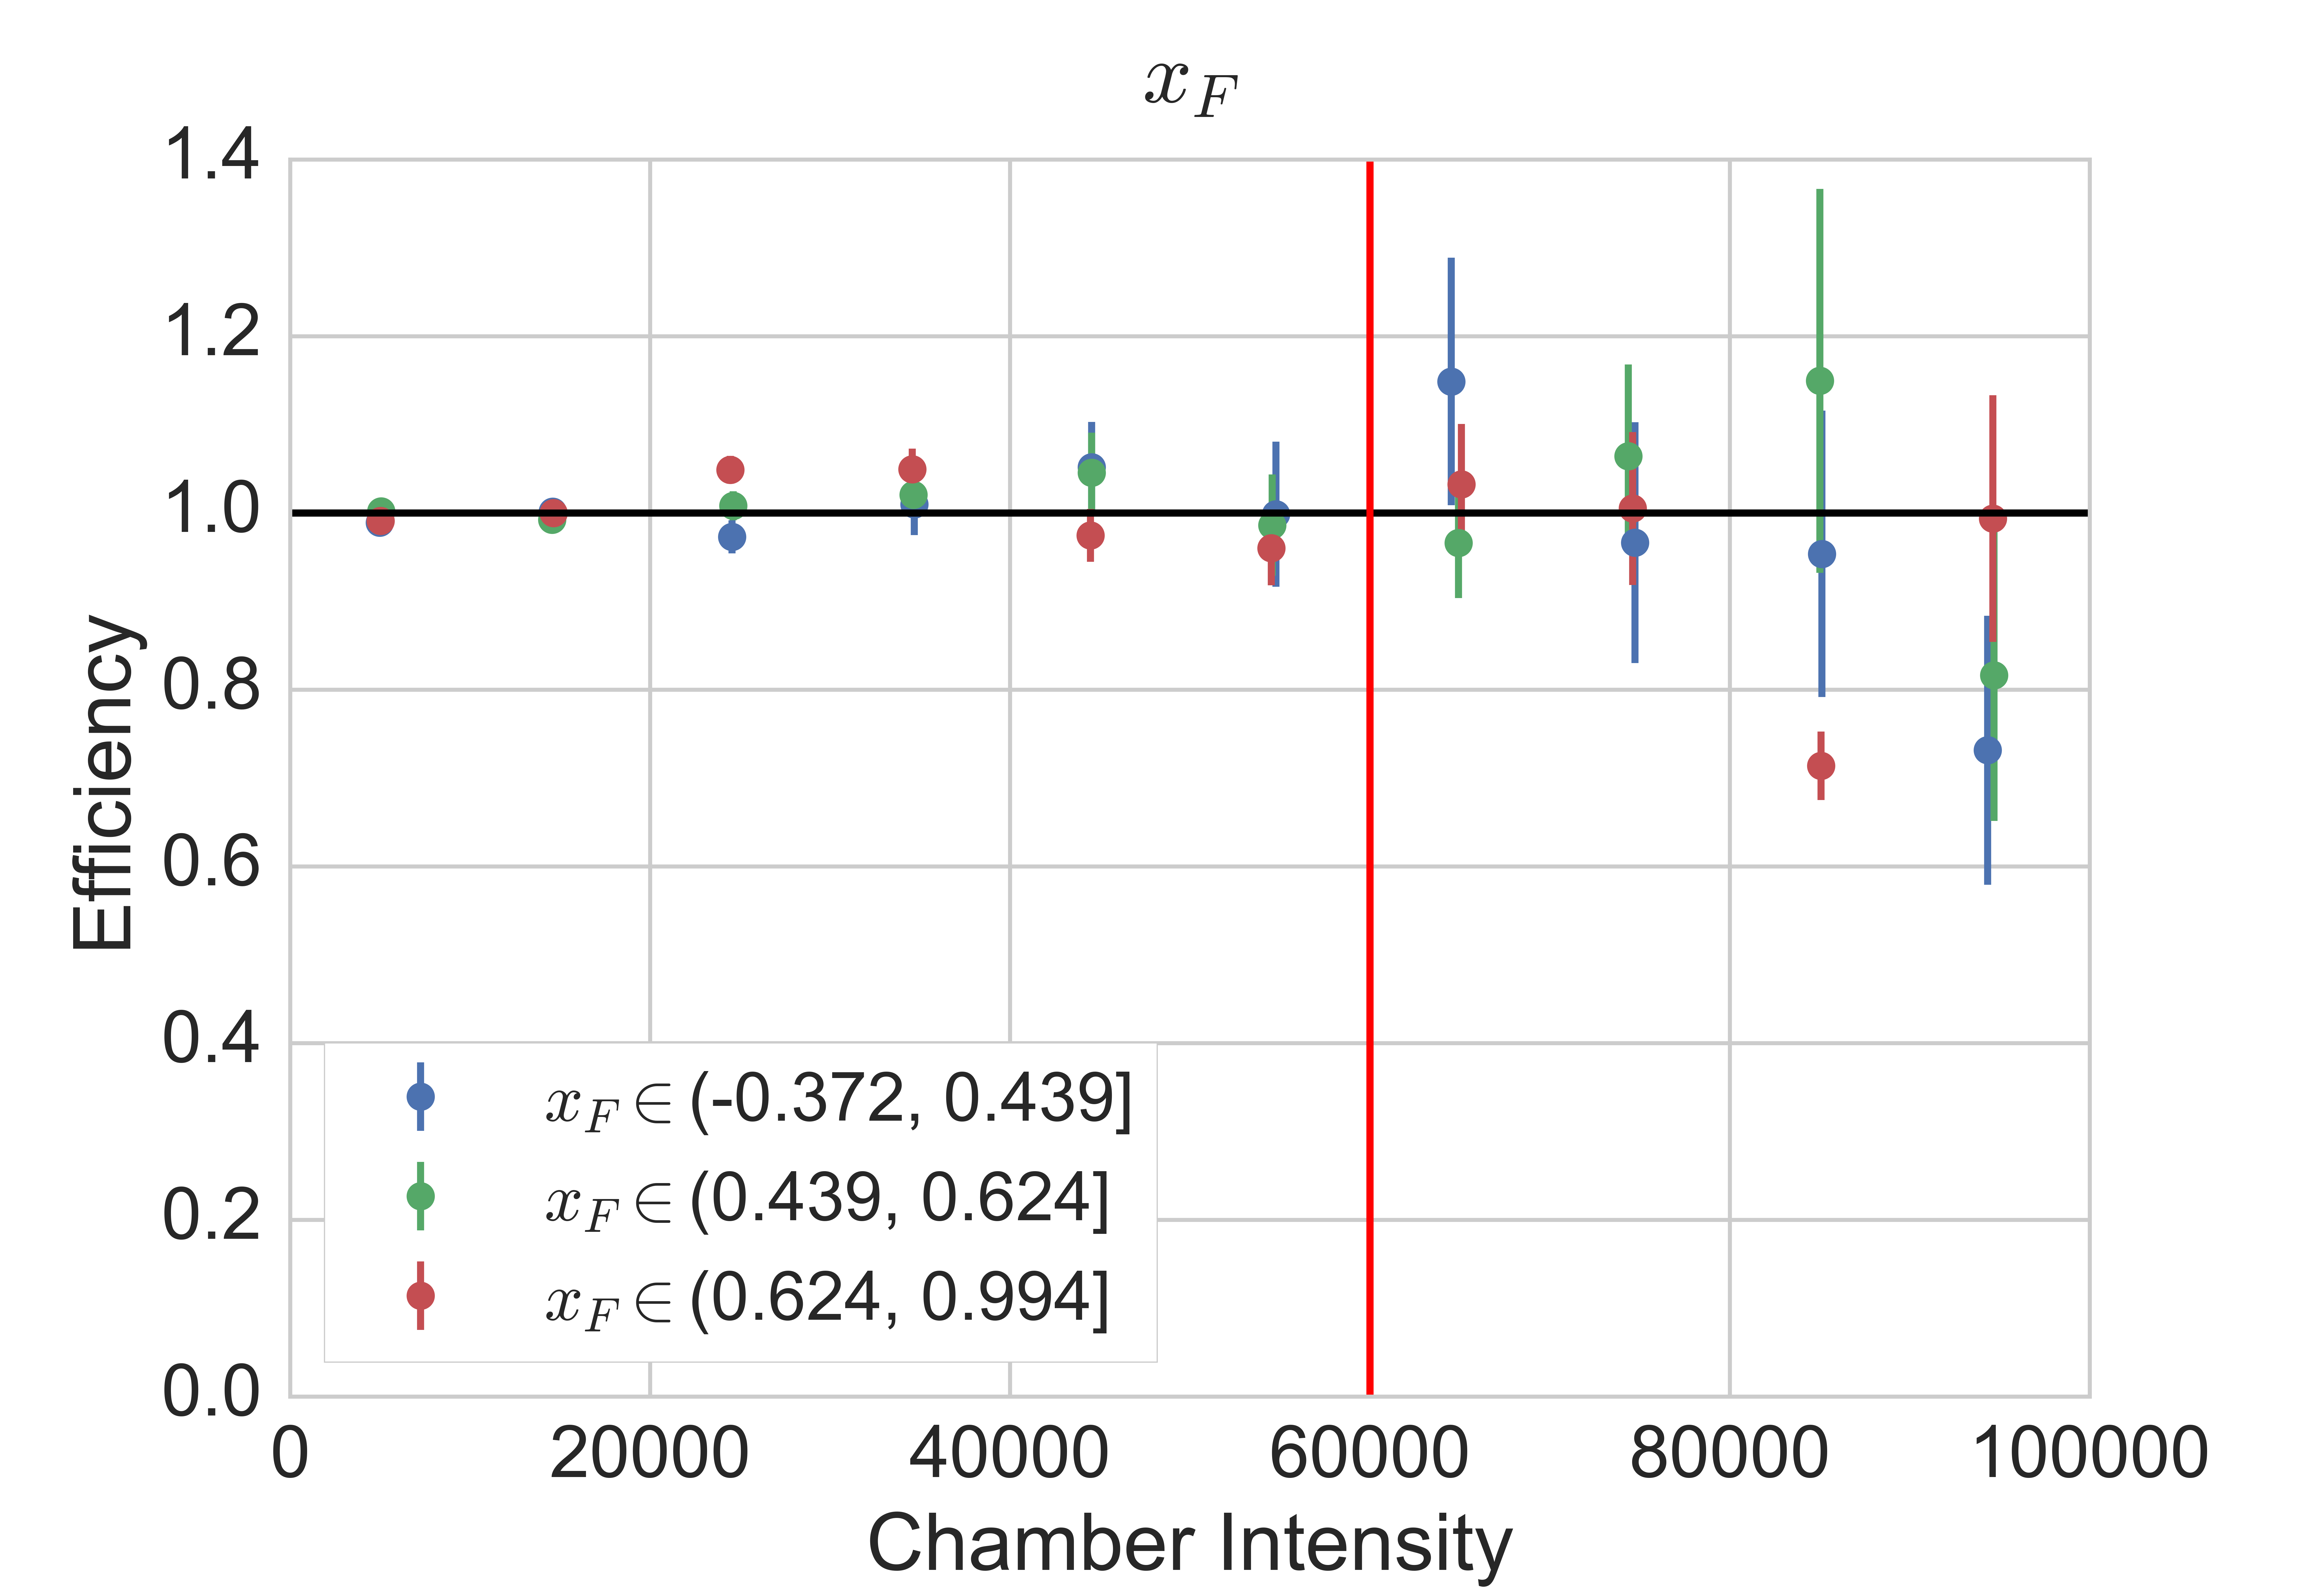
\includegraphics[width=0.49\textwidth]{figures/analysis/xF-keff-corrected-int.png}
	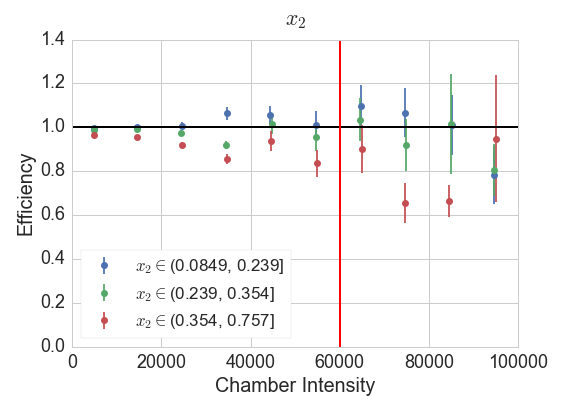
\includegraphics[width=0.49\textwidth]{figures/analysis/x2-keff-corrected-int.png}
	\caption{The efficiencies after re-weighting using kEfficiency values calculated when binned in $x_F$.}
	\label{fig:xf-keff-corrected}
\end{figure}
It should be noted that above approximately \unit[60,000]{protons} of chamber intensity, the tracking efficiency is low, and the weights become quite large. This combined with the fact that there are low statistics at high chamber intensity result in those events possessing a greater influence \emph{and} instability with respect to the yields. It is for this reason that events above this intensity threshold are removed from analysis. This boundary can be seen visually on Figure~\ref{fig:xf-keff-corrected}.

\begin{wraptable}{R}{0pt}
	\centering
	\begin{tabular}{lrrr}
		\toprule
		{} &        $A$ &        $\delta A$ &  $\chi^2/p.d.f.$ \\
		$x_2-$bin              &           &               &            \\
		\midrule
		(0.0856, 0.137] &  1.39e-05 &  4.08e-07 &   0.80 \\
		(0.137, 0.153]  &  1.50e-05 &  9.09e-07 &   2.32 \\
		(0.153, 0.168]  &  1.58e-05 &  5.67e-07 &   0.74 \\
		(0.168, 0.183]  &  1.45e-05 &  7.32e-07 &   1.62 \\
		(0.183, 0.202]  &  1.63e-05 &  6.77e-07 &   1.36 \\
		(0.202, 0.227]  &  1.69e-05 &  7.01e-07 &   2.00 \\
		(0.227, 0.269]  &  1.92e-05 &  7.71e-07 &   3.32 \\
		(0.269, 0.679]  &  2.24e-05 &  3.78e-07 &   1.65 \\
		\bottomrule
	\end{tabular}
	\caption{LD2 kEfficiency fit parameters with the $\chi^2$ evaluation of the fit to the data.}
	\label{tab:keff-ld2-fits}
\end{wraptable}
Another consideration is with respect to whether or not there is a target dependence to factor into the correction. For all of the above ``kEfficiency'' plots, only deuterium data is used. The kEfficiency curves for deuterium, hydrogen, carbon, iron, and tungsten can be found on Figure~\ref{fig:keff-target-roadset}. It can be concluded that there is enough of a difference between deuterium, iron, and the rest to justify calculating and applying this correction on a target-by-target basis.
\begin{figure}
	\centering
	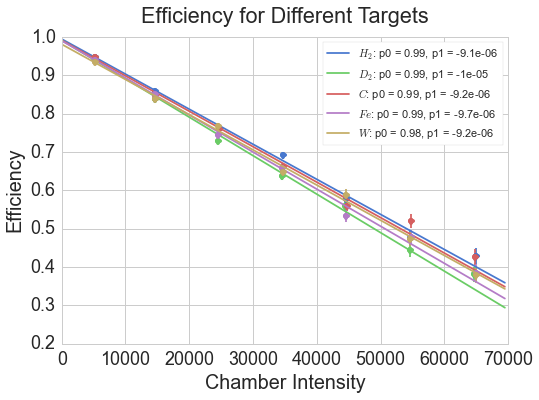
\includegraphics[width=0.49\textwidth]{figures/analysis/target-keff-int.png}
	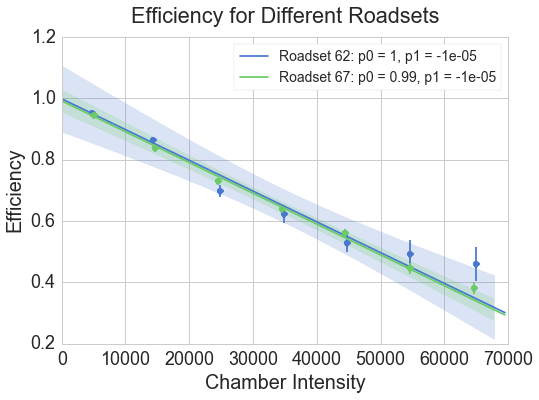
\includegraphics[width=0.49\textwidth]{figures/analysis/roadset-keff-int.png}
	\caption{Comparing the tracking efficiency curves across (left) the five targets and (right) two temporally different subsets (different roadsets) of data. Confidence bands removed from the target plot for the sake of clarity.}
	\label{fig:keff-target-roadset}
\end{figure}

Also, as a sanity check, there should be no time-dependence of this function. A quick check comparing different sets of data from two different roadsets quickly confirm that there is no such time dependence (Fig.~\ref{fig:keff-target-roadset}).

As a result, the final calculation of an tracking efficiency for a given dimuon event should depend on (1) target, (2) specific analysis kinematics, and (3) intensity. In order to apply this as a weight, we first define \emph{kEff}$_{t, \bar{x}}(I)$, a set of exponential fit functions: one for each target (\emph{t}) and for each kinematic bin ($\bar{x}$), which may be binned in any number of kinematic dimensions. The procedure in weighting each dimuon will then be to take each dimuon event \emph{i} and its chamber intensity $I_i$, originating from target $t_i$ in $\bar{x}_i$ bin $x_{F_i}$, create a weight as
\begin{equation}
w_i = \frac{1}{\text{kEff}_{t_i, \bar{x}_i}(I_i)}.
\end{equation}
When re-weighted in $x_2$ bins, the set of yields shown in Table~\ref{tab:raw-yields} can be updated to what is seen in Tables~\ref{tab:final-yields-57}, \ref{tab:final-yields-62}, and \ref{tab:final-yields-67} at the end of the chapter.

\subsection{ Empty Target Background Correction}\label{sec:bg}

Upon inspection, the Empty/None target data has shown to exhibit a rate dependence, with many more events per proton being found at higher intensities. This can be corrected for, but the events should first be weighted by their tracking efficiencies. Unfortunately since there are no \emph{messy/clean} embedded data sets for the empty flask, the ``kEfficiency'' fit must be extrapolated from the fits for the deuterium and hydrogen targets. If we are to assume that the difference in fits is a function of the beam's interaction with the target, then we can arrive at the \emph{kEff} exponential fit constants for the empty/none background targets ($A_{bg}$) for each kinematic bin from the exponential fit constants from the hydrogen and deuterium targets ($A_{D/H}$). Here, we only additionally need the number of interaction lenghts in the targets ($\xi$) to find the proportion of the beam that did not interact with the target ($X_t$) The values used can be found in Table~\ref{tab:targ-details}.
\begin{eqnarray}
X_t & = & 1 - e^{-\xi_t} \\
A_{bg} & = & A_H - X_H \cdot \frac{\Delta A}{\Delta X} \\
	   & = & A_H - X_H \cdot \frac{A_D - A_H}{X_D - X_H}
\end{eqnarray}

\begin{figure}
	\centering
	\includegraphics[width=0.7\textwidth]{figures/analysis/rate-dep-empty.png}
	\caption{The intensity-dependence of the Empty target and "None" target, with fit to $p_0 (1+p1\cdot I_c^2)$ for each. 95\% confidence band shown.}
	\label{fig:empty-rate-dep}
\end{figure}
With this fit constant in hand and the kEfficiency correction applied, one can plot the yields of empty flask and none events as a function of chamber intensity. This plot and its shape can be found in Figure~\ref{fig:empty-rate-dep}. Due to the low-statistics nature of the empty and none events, they are combined across all roadsets and kinematics instead of being broken down. As such, this correction is applied solely based on chamber intensity with no other consideration for roadset or kinematics. The fit that is applied is of the form: $f(I) = p_0 \cdot (1 + p_1 \cdot I_c^2)$. This form is chosen because the the scale of the final function will be a calculated from the data used, and as such, $p_1$ is the only parameter that is needed. The fit parameter $p_1$ was found to be:
\begin{eqnarray}
p^E_1 & = & (1.03 \pm 0.23) \times 10^{-9} \\
p^N_1 & = & (1.08 \pm 0.19) \times 10^{-9}.
\end{eqnarray}
The difference between the two backgrounds are interpreted to be due to interactions of the beam with the aluminum walls of the empty flask target.

\begin{wraptable}{R}{0pt}
	\centering
	\begin{tabular}{llrr}
		\toprule
		&             &  B &  $\delta$ B  \\
		Roadset & Target &                &       \\
		\midrule
		57 & LH2 &      0.119 &   0.014  \\
		&   LD2 &         0.057 &  0.006  \\
		& C &          0.046  &           0.004 \\
		& Fe &            0.019 &   0.002 \\
		& W &            0.017 &        0.002 \\ 
		\rowcol 62 & LH2 &      0.107 &   0.013  \\
		\rowcol &   LD2 &         0.051 &  0.006  \\
		\rowcol & C &          0.042 &           0.004 \\
		\rowcol & Fe &            0.019 &   0.002 \\
		\rowcol & W &            0.015 &        0.001 \\ 
		67 & LH2 &      0.095 &   0.011  \\
		&   LD2 &         0.039 &  0.005  \\
		& C &          0.043  &           0.004 \\
		& Fe &            0.018 &   0.002 \\
		& W &            0.015 &        0.001 \\ 
	\end{tabular}
	\caption{The calculated normalization constants for the background proportion function, C(I).}
	\label{tab:bg-b-vals}
\end{wraptable}
The fit function used, $C_{norm}(I_c) = B \cdot C(I_c) = B \cdot (1 + p_1 \cdot I_c)$  can be interpreted as \textbf{the probability that a given target dimuon actually arose from something other than a target interaction} (beam dump, upstream interactions, flask container). Here, $B$ is the normalization factor, where the condition should stand that the sum of $C_{norm}(I_c)$ over all target dimuons should be equal to the number of events from the empty and none targets. Both sums need to be corrected for kEffeciency and scaled by the number of live protons.
\begin{equation}
\sum\limits_T \frac{B \cdot C(I_c)}{P_T \cdot K_T(I_c)} = \sum\limits_E \frac{1}{P_E \cdot K_E(I_c)}
\end{equation}
\begin{eqnarray}
B & = & \frac{P_T}{P_E} \cdot \frac{\sum\limits_E \frac{1}{K_E(I_c)}}{\sum\limits_T \frac{C(I_c)}{K_T(I_c)}} \\
\delta B & = & \frac{P_T}{P_E} \cdot \frac{\sqrt{\sum\limits_E \frac{1}{K_E(I_c)^2}}}{\sum\limits_T \frac{C(I_c)}{K_T(I_c)}}
\end{eqnarray}
Here, $P_T$ is the live protons incident on target $T$ described in Table~\ref{tab:livep}, and $K_{(T/E)}(I_c)$ is the kEfficiency correction function. Calculated B-values for all targets and roadsets can be found in Table~\ref{tab:bg-b-vals}.

This normalization constant is calculated for each target and each roadset. With this in hand, a weight for correcting for the empty target correction can be applied as $(1 - C_{norm}(I_c^2))$, which can be interpreted as \textbf{the probability that the given dimuon arose from an actual target DY event}. One can then combine this with the weighting for the kEffeciency correction (as the weighting should combine multiplicatively):
\begin{equation}
\epsilon_{\text{tot}} = \epsilon_{\text{kEff}} \cdot \epsilon_{\text{empty}} = \frac{1 - C_{norm}(I_c)}{K_T(I_c)}
\end{equation}

It is worth noting that this model does not take into account the attenuation of beam throughout the different target materials, which could alter the scale of the correction slightly. However, without having a figure as to how much of the empty target signal comes from the beam dump and how much of it comes from upstream of the target area, it is currently infeasible to appropriately account for the degree to which a beam attenuation factor should be worked in.

Uncertainties that arise as a result of the uncertainties in the $C(I_x)$ fit and the calculation of $B$ are difficult to propagate analytically. What is performed instead is a an independent variation of $p_1$ and $B$ by $-1\sigma$, 0, and $+1\sigma$ and observing the magnitude of which the per nucleon cross section ratio changes as a result. This systematic uncertainty due to this correction is calculated in the Systematic Uncertainties section of this chapter.

\subsection{Residual Rate Dependent}

\begin{figure}
	\centering
	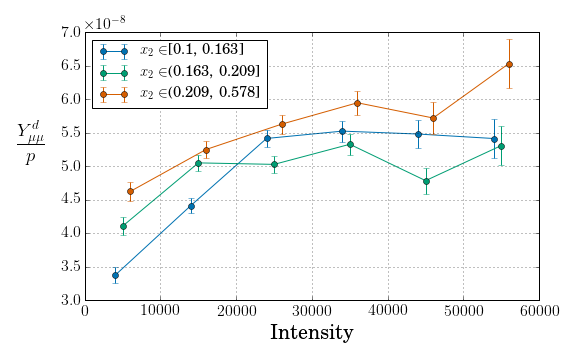
\includegraphics[width=0.48\textwidth]{figures/analysis/rate-dep-x2-after-corr.png}
	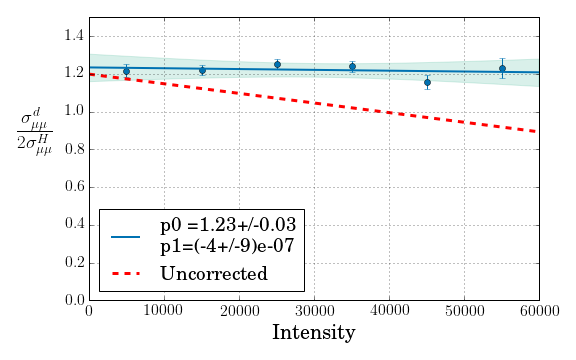
\includegraphics[width=0.48\textwidth]{figures/analysis/remaining-rate-dep.png}
	\caption{(Left) The remaining rate dependence behavior after corrections are made and (right) the rate dependence of a cross section ratio measurement with the linear fit and the 95\% confidence band shown.}
	\label{fig:residual-rate-dep}
\end{figure}

It should be emphasized that \emph{the issue of rate dependence is not a closed one}. As shown in this section, efforts have been put forth to make clever use of MC-generated data, tracking, and background information in order to identify and correct for as much of the rate dependence as possible. Due to the early nature of these approaches, there are bound to be factors which have yet to be accounted for, namely combinatoric backgrounds (uncorrelated single muons identified as signal dimuons). Plotting the yields per trigger proton again after both corrections (Fig.~\ref{fig:residual-rate-dep}, left), one can see that there is indeed still some rate dependence, but overall, the yields per proton no longer significantly decrease at higher intensities. Now the question is how to handle the residual rate dependence -- should an additional correction be applied, or should a systematic uncertainty be defined?

To decide, the cross section ratio measurement is taken and binned in chamber intensity. If the target-to-target and kinematic-dependent rate dependence is corrected, then this should be a flat line. The results as seen in Figure~\ref{fig:residual-rate-dep} (right) show that the ratio measurement is consistent with a line of zero slope. That is to say, the uncertainty in the slope is larger than the slope itself. Since this is the case, no further correction at this point will be applied, and a systematic uncertainty will be defined. Assuming that the rate dependence of the ratio measurement is a line, this is done by calculating the uncertainty of the fit $\sigma_f$ over the value of the fit at the mean chamber intensity value. It should be noted that $\sigma_f$ benefits from negative off-diagonal covariance elements for the fit parameters.

The systematic uncertainty here is calculated to be 1.07\% of the cross section ratios.

\section{LD2 Contamination}\label{sec:contam}

During Run III of the SeaQuest experiment, analysis of the deuterium source used indicated that it was impure to a significant degree. This calls for a significant correction since most measurements, yields, ratios, and analyses assume that the targets are pure. An impure deuterium target changes many factors including the averaged mass number of the fluid and its overall density. In this section, the contamination measurements and the correction procedure is discussed.

\subsection{Contamination Measurements}

The SeaQuest deuterium target was emptied and filled several times during data taking. At each of these times, a sample was taken from either the target or from the deuterium gas cylinder used to fill the target. These samples were sent to Los Alamos for isotopic analysis where each sample was analyzed twice. The results of these analyses are shown in Table~\ref{tab:deut-contam}. In each case of parallel analyses on a single gas sample, the two results were in agreement. Upon examination of the deuterium compositions, some problems are immediately clear. Specifically, the ratios of $H_2$, $HD$, and $D_2$ are different between the three samples, but the bottles were supposed to have been filled from the same source many years ago. Second, some of the samples had a significant contribution of other gases, including $N_2$ and $O_2$. This indicates an additional contamination of air. A sample of the first $H_2$ target was analyzed and found to be $\sim98\%$ pure with negligible contributions from other species.

\begin{table}
	\centering
	\begin{tabular}{@{}rrrrrrrrrr@{}}
		\toprule
		{} & \textbf{Runs:} & \multicolumn{2}{c}{3230-11143} & \phantom{abc} & \multicolumn{2}{c}{11144-11477} & \phantom{abc} & \multicolumn{2}{c}{11478-14652} \\ \cmidrule{3-4} \cmidrule{6-7} \cmidrule{9-10}
		\textbf{Species:} & \textbf{Test:} & \multicolumn{1}{c}{1} & \multicolumn{1}{c}{2} & & \multicolumn{1}{c}{1} & \multicolumn{1}{c}{2} & & \multicolumn{1}{c}{1} & \multicolumn{1}{c}{2} \\ \midrule
		$H_2$	& & 1.23 & 1.225 					& & 0.25 & 0.25 				& & 4.603 & 4.591 \\
		$HD$		  & & 16.187 & 16.171 						& & 8.393 & 8.391 			   & & 6.983 & 6.982 \\
		$D_2$ 	& & 79.78 & 79.729 			 	  & & 90.871 & 90.808 			& & 80.504 & 80.443 \\
		$He$ 		   & & 2.20 & 2.188 		 		 	   & & 0.018 & 0.014 				& & $<$0.01 & $<$0.01 \\
		$CH_4$ & & $<$0.009 & $<$0.009 	   & & $<$0.007 & $<$0.007 	 & & $<$0.008 & $<$0.008 \\
		$H_2O$ 	& & $<$0.009 & 0.073   			& & 0.038 & 0.099 			   & & 0.033 & 0.061 \\
		$HDO$ 	 & & 0.015 & 0.026 					& & 0.024 & 0.033 				& & 0.021 & 0.04 \\
		$D_2O$ & & $<$0.007 & $<$0.009      & & $<$0.007 & $<$0.008   & & $<$0.009 & $<$0.012 \\
		$Ne$ 		   & & 0.007 & 0.065 		   		  & & $<$0.027 & $<$0.027 	& & $<$0.03 & $<$0.03 \\
		$N_2$ 	& & 0.428 & 0.419 				    & & 0.323 & 0.323 			   & & 6.395 & 6.382 \\
		$C_2H_6$ & & $<$0.006 & $<$0.006   & & $<$0.005 & $<$0.005   & & $<$0.006 & $<$0.006 \\
		$O_2$ 	& & 0.085 & 0.098 			 	  		   & & 0.068 & 0.068 			   & & 1.389 & 1.416 \\
		$Ar$ 			& & 0.005 & 0.006 				 		  & & 0.004 & 0.003 			  & & 0.063 & 0.064 \\
		$CO_2$ & & $<$0.002 & $<$0.002	    & & 0.011 & 0.009 				 & & 0.01 & 0.01 \\
		$C_3H_8$ & & $<$0.006 & $<$0.006  & & $<$0.005 & $<$0.005   & & $<$0.006 & $<$0.006 \\
		\bottomrule
	\end{tabular}
	\caption{Results of the isotropic analyses of the liquid deuterium samples. Two tests are applied to each sample, and all numbers are in percentages.}
	\label{tab:deut-contam}
\end{table}

The source of the deuterium used at SeaQuest is from a bubble chamber experiment at Fermilab. At some undocumented point in the past, the contents of the bubble chamber were transferred into a tube trailer for storage. At a later time, the $D_2$ was transferred into cylinders for storage. Discussions with gas storage experts indicate that there was likely no special treatment of the cylinders other than being evacuated when they were filled with $D_2$, with the desired special treatment being to ``bake'' the cylinders, or heat them up to release residual hydrogen that tends to diffuse into the metal surface of their inner walls. In addition to that, the containers used to take samples from the target or cylinders were also not ``baked,'' so existing estimates of the contamination may \emph{only} be from the sampling containers -- or the contamination could be doubly worsened by contamination in the sampling containers. As such, effects of this contamination are treated as a systematic error with asymmetric uncertainties. After run 14652, a commercial deuterium gas has been used which has an analyzed purity of $>99.9999\%$, and no systematic uncertainty will need be applied.

Contamination from air in the sample gases is unlikely to have come from the targets. Prior to filling, the targets undergo several cycles of evacuation and refilling with deuterium before the final fill is done. This cycle should flush out all residual air from the target flask. Further, if there was air supply being fed into the target, all but the lowest temperature gases should have been removed by the liquid nitrogen ``cold trap.'' Aside from hydrogen isotopes, helium is the only other component found in the samples. Since the target temperature were approximately \unit[23]{K}, any helium would have been in a gas state and not in the bulk liquid in the flask. Thus, the gases from the analysis shown in Table~\ref{tab:deut-contam} can be renormalized to consider only the hydrogen isotopes, which can be seen in Table~\ref{tab:deut-contam-renorm}.

\begin{table}
	\centering
	\begin{tabular}{@{}rlrrr@{}}
		\toprule
		{} & \textbf{Run} & \multicolumn{1}{c}{3230-} & \multicolumn{1}{c}{11144-} &  \multicolumn{1}{c}{11478} \\ 
		{} & \textbf{Range:} & \multicolumn{1}{c}{11143} & \multicolumn{1}{c}{11477} &  \multicolumn{1}{c}{14652} \\ 
		\textbf{Species:} & & & & \\ \midrule
		$H_2$	& & 1.26   & 0.25  & 4.99 \\
		$HD$    & & 16.65 & 8.44  &	 7.59 \\
		$D_2$ 	& & 82.08 & 91.31 &  87.42 \\
		\bottomrule
	\end{tabular}
	\caption{Renormalized compositions (in percentages) when considering only the hydrogen isotopes.}
	\label{tab:deut-contam-renorm}
\end{table}

Until the true compositions can be ascertained, it has been recommend that analyses use the atomic percentages provided by the Los Alamos analysis as shown in Table~\ref{tab:deut-atomic-perc}, which represents the best understanding of the deuterium at this point. To assign a systematic uncertainty to these numbers, the recommended approach is to use asymmetric uncertainties, assuming that one the extreme values for H and D. Due to the fact that there is a complete inverse correlation between hydrogen and deuterium an uncertainty is assigned to the deuteron percentage only.

\begin{table}
	\centering
	\begin{tabular}{@{}rlrrrr@{}}
		\toprule
		{} & \textbf{Run} & \multicolumn{1}{c}{3230-} & \multicolumn{1}{c}{11144-} &  \multicolumn{1}{c}{11478-} & \multicolumn{1}{c}{14653-}  \\ 
		{} & \textbf{Range:} & \multicolumn{1}{c}{11143} & \multicolumn{1}{c}{11477} &  \multicolumn{1}{c}{14652} & \multicolumn{1}{c}{Present} \\ 
		\textbf{Atom:} & & & & & \\ \midrule
		$H$	& & 9.6   & 4.5  & 8.8 & 0.0 \\
		$D$    & & $90.4^{+5}_{-0}$ & $95.5^{+0}_{-5}$  & $91.2^{+4}_{-1}$ & 100.0 \\
		\bottomrule
	\end{tabular}
	\caption{Atomic percentages of the deuterium targets with asymmetric uncertainties in the $d$ percentage.}
	\label{tab:deut-atomic-perc}
\end{table}

\subsection{Contamination Correction}

With the assumption that the heavier atoms are caught in the cold trap and the gaseous helium stays at the top of the flask and away from the path of the proton beam, a contamination correction is implemented based on the atomic percentage composition detailed in Table~\ref{tab:deut-atomic-perc}. The nuclear interaction length, density, and atomic mass of the liquid deuterium target is corrected based on the cotamination. With $A$ as the atomic mass, $\lambda$ as the nuclear interaction length, $\rho$ as the density, and $F_{H/D}$ as the proportion of $H$ or $D$ in the target, the following are assumed to be approximately true:

\noindent\begin{minipage}{.5\linewidth}
	\begin{eqnarray}
	A & = & A_H\cdot F_H + A_D \cdot F_D \\
	\rho & = & \rho_H\cdot F_H + \rho_D \cdot F_D
	\end{eqnarray}
\end{minipage}%
\begin{minipage}{.5\linewidth}
	\begin{eqnarray}
	\frac{1}{\lambda } & = & \frac{F_H}{\lambda_H} + \frac{F_D}{\lambda_D} \\
	\lambda & = & \frac{\lambda_H \cdot \lambda_D}{F_H \cdot \lambda_D + F_D \cdot \lambda_H}	
	\end{eqnarray}
\end{minipage}
\newline

Due to the contamination, some of the signal events with the liquid deuterium target in place will actually come from hydrogen instead of a deuteron. With $\hat{\sigma}_{pH}$ and $\hat{\sigma}_{pD}$ representing the \emph{measured} target cross section, and $\sigma_{pp}$ and $\sigma_{pn}$ representing the proton-proton and proton-neutron cross section, 

\noindent\begin{minipage}{.5\linewidth}
	\begin{eqnarray}
	\hat{\sigma}_{pH} & = & a \cdot \sigma_{pp} + b \cdot \sigma_{pn} \\
	\hat{\sigma}_{pD} & = & c \cdot \sigma_{pp} + d \cdot \sigma_{pn}
	\end{eqnarray}
\end{minipage}%
\begin{minipage}{.5\linewidth}
	\begin{eqnarray}
	\sigma_{pp} & = & \frac{b \cdot \hat{\sigma}_{pD} - d \cdot \hat{\sigma}_{pH}}{b \cdot c - a \cdot d} \\
	\sigma_{pn} & = & \frac{a \cdot \hat{\sigma}_{pD} - c \cdot \hat{\sigma}_{pH}}{a \cdot d - b \cdot c}
	\end{eqnarray}
\end{minipage}
\newline

\noindent Here, the coefficients $a, b, c,$ and $d$ denote the number of protons and neutrons per atom for the different targets. We know that $a=c=1$, and since the hydrogen target is considered to be pure, $b=0$. The remaining value, $d$, is the fraction of deuteron atoms in the sample ($F_D$ above). With this, we can arrive at an expression for $\sigma_{pD}^{\text{pure}}$.
\begin{eqnarray}
\sigma_{pH}^{\text{pure}} & = & \sigma_{pp} = \hat{\sigma}_{pH} \\
\sigma_{pn} & = & \frac{\hat{\sigma}_{pD} - \hat{\sigma}_{pH}}{d} \\
\sigma_{pD}^{\text{pure}} & = & \sigma_{pp} + \sigma_{pn} \\
\sigma_{pD}^{\text{pure}} & = & \frac{\hat{\sigma}_{pD} - \hat{\sigma}_{pH}\cdot (1-d)}{d} \label{eq:contam-corr}
\end{eqnarray}

In practice, this correction is applied bin-by-bin, utilizing the weighted dimuon yield for each target in place of $\hat{\sigma}$. The $d$ used depends on the run ranges applicable to the roadset being analyzed, and the values are derived from those in Table~\ref{tab:deut-atomic-perc}. It's the case that the deuterium was changed in the middle of the roadset -- twice for Roadset 62 and twice again for for Roadset 67. As a result, the contaminations are averaged, proportional to the number of runs with a given sample, and generous systematic uncertaies are allowed with the understanding that the deuterium compositions will be re-analyzed and known more exactly in the future. The values of $91.3\pm4\%$ is used for Roadset 62 and $95.3\pm3\%$ is used for Roadset 67. In order to arrive at a systematic uncertainty due to the uncertainty in the knowledge of the contamination, the analysis is performed at the with values at nominal, $+\sigma$, and $-\sigma$ are perfomed, with the largest \% change in the ratio value to be valued as the systematic uncertainty.

\section{\texorpdfstring{Isoscalar Corrections for $^{183}W$ and $^{56}Fe$}{Isoscalar Corrections for W-183 and Fe-56 }}

\begin{figure}
	\centering
	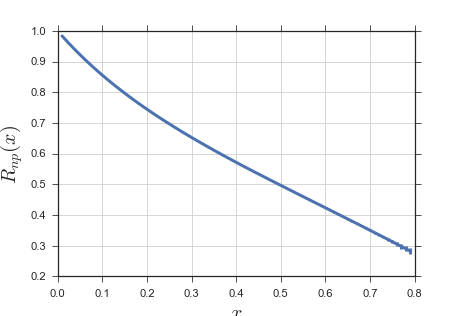
\includegraphics[width=0.48\textwidth]{figures/analysis/rnp.png}
	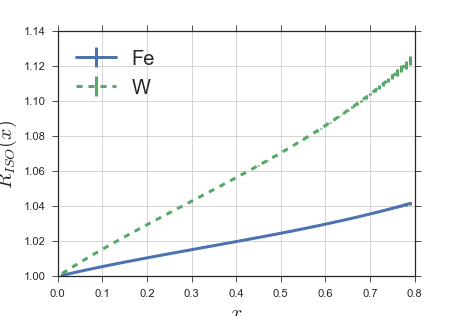
\includegraphics[width=0.48\textwidth]{figures/analysis/riso.png}
	\caption{(Left) The ratio of free neutron to proton $F_2$ structure functions following a detailed parametrization~\cite{Arrington:2008zh} and the isoscalar correction factor~\cite{Hen:2013oha}, $R_{ISO}(x)$, for iron and tungsten.}
	\label{fig:rnp-riso}
\end{figure}

The proton and neutron are similar in many ways, but they do not share the same $F_2$ structure function. This is primarily due it being a charge-weighted summation of its quark constituents. So, taking the ratio of cross sections for asymmetric nuclei ($N\neq Z$) to deuterium ($N=Z=1$) will not result in a proper extraction of the ratio of $F_2$. to correct for this, following Aubert \emph{et al.} and Bodek \emph{et al.}~\cite{Aubert:1983xm, PhysRevLett.50.1431}, an additional isoscalar correction factor ($R_{ISO}$) is applied to the yield ratio, approximating the ratio to a hypothetical nucleus with equal numbers of protons and neutrons ($N=Z=A/2$):
\begin{equation}
\frac{\sigma^A_{DY}(x, Q^2)_{ISO}}{\sigma^D_{DY}(x, Q^2)_{ISO}} = \frac{\sigma^A_{DY}(x, Q^2)}{\sigma^D_{DY}(x, Q^2)} \cdot R_{ISO}(x, A, Z)
\end{equation}
where $R_ISO(x, A, Z)$ is expressed as
\begin{equation}
R_{ISO}(x, A, Z) = \frac{A}{2} \cdot \frac{F_2^p(x, Q^2) + F_2^n(x, Q^2)}{Z\cdot F_2^p(x, Q^2) + N\cdot F_2^n(x,Q^2)} = \frac{A}{2} \cdot \frac{1+R_{np}(x, Q^2)}{Z + N\cdot R_{np}(x, Q^2)}
\end{equation}
and $R_{np}(x)$ is defined as
\begin{equation}
R_{np}(x,Q^2) = \frac{F_2^n(x,Q^2)}{F_2^p(x,Q^2)}.
\end{equation}
The ratio of the free nucleon structure functions for neutrons to protons is extracted from world data on DIS scattering~\cite{Arrington:2008zh}  off of deuterium and hydrogen with corrections accounting for Fermi motion of nucleons in deuterium. The behavior of $R_{np}(x)$ and $R_{ISO}(x, A, Z)$ for the case of iron can be seen in Figure~\ref{fig:rnp-riso}.

\section{Summary of Analysis Steps}

Due to the dynamic nature of the SeaQuest analysis at the time of the writing of this document, it is imporant to lay out the precise procedure of the application of all of these analysis steps. This ensures an ability to reproduce results, understand differences between methods, and allows those new to analysis to have a roadmap for getting started with analysis. Pragmatically speaking, the process taken in this analysis going from the raw dimuon yields to the final extraction of $F_2^A(x)/F_2^D(x)$ can be outlined in several finite steps:
\begin{enumerate}
	\item Get raw yields after all analysis cuts (Chapter~\ref{chap:track-data-cuts}).
	\item Get live proton count (Section~\ref{sec:livep}).
	\item Calculate the kEfficiency and apply it for all (non-BG) targets (Section~\ref{sec:keff}).
	\item Extrapolate kEfficiency for Empty/None target. (Section~\ref{sec:bg})
	\item Calculate $C(I_c)$ and $B_T$ empty target correction fit and parameters (Section \ref{sec:bg}).
	\item Calculate weighted yields:
	\begin{equation}
	Y_T^\prime = \sum\limits_T \frac{1 - B_T \cdot C(I_c)}{K_T(I_c)}
	\end{equation}
	\item Adjust the deuterium yields for the hydrogen contamination (Equation~\ref{eq:contam-corr}).
	\item Normalize each targets' yields for each roadset according to the number of live protons ($P_A$) on target (Section~\ref{sec:livep}).
	\item Take ratios of these adjusted, normalized yields:
	\begin{equation}
		\frac{Y_A^\prime / P_A}{Y_D^\prime / P_D}
	\end{equation}
	\item Apply the remaining compnents of the target-to-target normalization factor to the ratio (Section~\ref{sec:targ-to-targ-norm}):
	\begin{equation}
	N_{A/D} =
	\left( \frac{ 2 \cdot n_D \cdot L^D \cdot T^D(\xi)}{ A \cdot n_A \cdot L^A \cdot T^A(\xi)} \right) \cdot 
	\cancelto{1}{\frac{ \varepsilon^D }{ \varepsilon^A }}  \cdot 
	\cancelto{0.9989}{\frac{ \bar{\Omega}^D }{\bar{ \Omega}^A }}
	\end{equation}
	\item With asymmetric nuclei ($^{56}Fe, ^{184}W$), apply $R_{ISO}(x)$ isoscalar correction factor using the mean $x_2$ value in that ratio bin.
\end{enumerate}
This procedure is general enough that it can be performed with any kinematic binning.

\section{Corrected, Aggregated Yields}

After all corrections are implemented, presented here are the per-live proton yields for the three analyzed roadsets, 57, 62, and 67, binned in $x_2$ (Tables~\ref{tab:final-yields-57}, \ref{tab:final-yields-62}, and \ref{tab:final-yields-67}).  The yields here are for the case of kEfficiency corrections in the $x_2$ kinematic. With this data in hand, by the above steps, we can arrive at our cross section ratio measurmements. Also shown here (Table~\ref{tab:contam-correct-table}) is the effect of applying the target contamination correction for the nominal value of the contamination for each roadset.

Before we do so, it is important to ensure that these results are able to be combined. This can be confirmed by investigating the \emph{time-dependence} of the distributions. In this case, this would be comparing the kinematic distributions for different roadsets. This comparison is made in Figures~\ref{fig:roadset-x2-compare}, \ref{fig:roadset-x1-compare}, \ref{fig:roadset-mass-compare}, and \ref{fig:roadset-xF-compare} where the normalized distributions for $x_2, x_1, M_{\gamma^*},$ and $x_F$ for different pairs of roadsets are shown against each other. The difference between distributions are overlaid on each plot, with the red line showing the location of zero with respect to the difference. Overall, the distributions possess the same shape across all roadsets and the $chi^2/p.d.f.$ values are acceptably low. 

\begin{table}
	\centering
	\caption*{\textbf{Roadset 57: All Yields Normalized to Live Protons}}
\begin{tabular}{lllll}
	\toprule
	&             &      Raw Yields &  kEff-Corrected &   kEff+BG Corrected \\
	Target & $x_2$ &                    &            Yields        &                Yields    \\
	\midrule
	LH2 & (0.1, 0.13] &             60$\pm$4 &             89$\pm$6 &             69$\pm$4 \\
	& (0.13, 0.16] &            164$\pm$6 &           240$\pm$10 &            188$\pm$7 \\
	& (0.16, 0.195] &            193$\pm$7 &           281$\pm$10 &            221$\pm$8 \\
	& (0.195, 0.24] &            147$\pm$6 &           225$\pm$10 &            176$\pm$7 \\
	& (0.24, 0.29] &             79$\pm$4 &            132$\pm$8 &            102$\pm$6 \\
	& (0.29, 0.35] &         42.5$\pm$3.2 &             71$\pm$6 &             56$\pm$4 \\
	& (0.35, 0.45] &         14.4$\pm$1.9 &         24.9$\pm$3.5 &         19.1$\pm$2.6 \\
	& (0.45, 0.58] &          2.0$\pm$0.7 &          3.8$\pm$1.4 &          2.8$\pm$1.0 \\
\rowcol 	LD2 & (0.1, 0.13] &            137$\pm$8 &           194$\pm$12 &           186$\pm$12 \\
\rowcol 	& (0.13, 0.16] &           370$\pm$14 &           545$\pm$20 &           522$\pm$20 \\
\rowcol 	& (0.16, 0.195] &           430$\pm$15 &           611$\pm$21 &           589$\pm$21 \\
\rowcol 	& (0.195, 0.24] &           329$\pm$13 &           503$\pm$20 &           482$\pm$20 \\
\rowcol 	& (0.24, 0.29] &            173$\pm$9 &           282$\pm$16 &           271$\pm$16 \\
\rowcol 	& (0.29, 0.35] &             91$\pm$7 &           161$\pm$13 &           154$\pm$12 \\
\rowcol 	& (0.35, 0.45] &             43$\pm$5 &             74$\pm$8 &             71$\pm$8 \\
\rowcol 	& (0.45, 0.58] &          7.4$\pm$1.9 &         12.7$\pm$3.5 &         12.4$\pm$3.4 \\
	C & (0.1, 0.13] &            111$\pm$9 &           161$\pm$14 &           146$\pm$12 \\
	& (0.13, 0.16] &           277$\pm$15 &           429$\pm$23 &           392$\pm$21 \\
	& (0.16, 0.195] &           340$\pm$16 &           500$\pm$25 &           458$\pm$22 \\
	& (0.195, 0.24] &           252$\pm$14 &           391$\pm$22 &           357$\pm$20 \\
	& (0.24, 0.29] &           129$\pm$10 &           224$\pm$18 &           203$\pm$16 \\
	& (0.29, 0.35] &             65$\pm$7 &           111$\pm$13 &           102$\pm$12 \\
	& (0.35, 0.45] &             33$\pm$5 &             53$\pm$8 &             49$\pm$8 \\
	& (0.45, 0.58] &          1.5$\pm$1.1 &          2.1$\pm$1.5 &          2.0$\pm$1.4 \\
\rowcol 	Fe & (0.1, 0.13] &           271$\pm$26 &    (3.9$\pm$0.4)e+02 &    (3.8$\pm$0.4)e+02 \\
\rowcol 	& (0.13, 0.16] &    (6.7$\pm$0.4)e+02 &  (1.03$\pm$0.06)e+03 &    (9.9$\pm$0.6)e+02 \\
\rowcol 	& (0.16, 0.195] &    (8.4$\pm$0.5)e+02 &  (1.31$\pm$0.07)e+03 &  (1.26$\pm$0.07)e+03 \\
\rowcol 	& (0.195, 0.24] &    (6.4$\pm$0.4)e+02 &    (9.9$\pm$0.6)e+02 &    (9.6$\pm$0.6)e+02 \\
\rowcol 	& (0.24, 0.29] &           304$\pm$27 &    (5.0$\pm$0.5)e+02 &    (4.8$\pm$0.5)e+02 \\
\rowcol 	& (0.29, 0.35] &           219$\pm$23 &    (3.7$\pm$0.4)e+02 &    (3.6$\pm$0.4)e+02 \\
\rowcol 	& (0.35, 0.45] &            78$\pm$14 &           135$\pm$25 &           130$\pm$24 \\
\rowcol 	& (0.45, 0.58] &             12$\pm$5 &            26$\pm$12 &            25$\pm$12 \\
	W & (0.1, 0.13] &           267$\pm$25 &    (4.1$\pm$0.4)e+02 &    (4.0$\pm$0.4)e+02 \\
	& (0.13, 0.16] &    (7.3$\pm$0.4)e+02 &  (1.12$\pm$0.07)e+03 &  (1.09$\pm$0.06)e+03 \\
	& (0.16, 0.195] &  (1.00$\pm$0.05)e+03 &  (1.53$\pm$0.08)e+03 &  (1.48$\pm$0.07)e+03 \\
	& (0.195, 0.24] &    (6.9$\pm$0.4)e+02 &  (1.12$\pm$0.07)e+03 &  (1.09$\pm$0.07)e+03 \\
	& (0.24, 0.29] &           368$\pm$30 &    (6.1$\pm$0.5)e+02 &    (5.9$\pm$0.5)e+02 \\
	& (0.29, 0.35] &           230$\pm$24 &    (4.1$\pm$0.4)e+02 &    (3.9$\pm$0.4)e+02 \\
	& (0.35, 0.45] &            76$\pm$14 &           142$\pm$27 &           137$\pm$26 \\
	& (0.45, 0.58] &             12$\pm$6 &            22$\pm$10 &            21$\pm$10 \\
	\bottomrule
\end{tabular}
	\caption{Total yields for each target for each $x_2$ bin normalized to the live protons on target. The LD2 has also been corrected for contamination in the last column.}
	\label{tab:final-yields-57}
\end{table}

\begin{table}
	\centering
	\caption*{\textbf{Roadset 62: All Yields Normalized to Live Protons}}
\begin{tabular}{lllll}
	\toprule
	&             &      Raw Yields &  kEff-Corrected &   kEff+BG Corrected \\
	Target & $x_2$ &                    &            Yields        &                Yields    \\
	\midrule
	LH2 & (0.1, 0.13] &             70$\pm$4 &            102$\pm$5 &             83$\pm$4 \\
	& (0.13, 0.16] &            184$\pm$6 &            272$\pm$9 &            218$\pm$7 \\
	& (0.16, 0.195] &            229$\pm$6 &           341$\pm$10 &            274$\pm$8 \\
	& (0.195, 0.24] &            182$\pm$6 &            281$\pm$9 &            226$\pm$7 \\
	& (0.24, 0.29] &            104$\pm$4 &            174$\pm$8 &            139$\pm$6 \\
	& (0.29, 0.35] &         48.7$\pm$3.0 &             86$\pm$6 &             69$\pm$4 \\
	& (0.35, 0.45] &         19.5$\pm$1.9 &         33.2$\pm$3.4 &         26.7$\pm$2.7 \\
	& (0.45, 0.58] &          3.3$\pm$0.8 &          5.5$\pm$1.4 &          4.5$\pm$1.1 \\
\rowcol 	LD2 & (0.1, 0.13] &            157$\pm$8 &           230$\pm$12 &           221$\pm$12 \\
\rowcol 	& (0.13, 0.16] &           413$\pm$13 &           612$\pm$20 &           590$\pm$19 \\
\rowcol 	& (0.16, 0.195] &           516$\pm$15 &           763$\pm$22 &           737$\pm$22 \\
\rowcol 	& (0.195, 0.24] &           389$\pm$13 &           603$\pm$20 &           580$\pm$20 \\
\rowcol 	& (0.24, 0.29] &            193$\pm$9 &           328$\pm$16 &           313$\pm$16 \\
\rowcol 	& (0.29, 0.35] &            110$\pm$7 &           204$\pm$13 &           195$\pm$13 \\
\rowcol 	& (0.35, 0.45] &             49$\pm$4 &             86$\pm$8 &             83$\pm$8 \\
\rowcol 	& (0.45, 0.58] &          5.7$\pm$1.5 &         10.0$\pm$2.7 &          9.6$\pm$2.8 \\
	C & (0.1, 0.13] &           100$\pm$10 &           146$\pm$14 &           134$\pm$13 \\
	& (0.13, 0.16] &           322$\pm$17 &           511$\pm$28 &           470$\pm$26 \\
	& (0.16, 0.195] &           433$\pm$20 &           653$\pm$31 &           603$\pm$28 \\
	& (0.195, 0.24] &           345$\pm$18 &           539$\pm$29 &           497$\pm$26 \\
	& (0.24, 0.29] &           196$\pm$13 &           316$\pm$22 &           293$\pm$21 \\
	& (0.29, 0.35] &             92$\pm$9 &           159$\pm$17 &           147$\pm$15 \\
	& (0.35, 0.45] &             38$\pm$6 &            66$\pm$11 &            61$\pm$10 \\
	& (0.45, 0.58] &          7.4$\pm$2.6 &             11$\pm$4 &             11$\pm$4 \\
\rowcol 	Fe & (0.1, 0.13] &           273$\pm$23 &           415$\pm$35 &           399$\pm$34 \\
\rowcol 	& (0.13, 0.16] &    (7.5$\pm$0.4)e+02 &  (1.15$\pm$0.06)e+03 &  (1.11$\pm$0.06)e+03 \\
\rowcol 	& (0.16, 0.195] &    (9.6$\pm$0.4)e+02 &  (1.53$\pm$0.07)e+03 &  (1.48$\pm$0.07)e+03 \\
\rowcol 	& (0.195, 0.24] &    (7.8$\pm$0.4)e+02 &  (1.22$\pm$0.06)e+03 &  (1.17$\pm$0.06)e+03 \\
\rowcol 	& (0.24, 0.29] &           402$\pm$28 &    (7.1$\pm$0.5)e+02 &    (6.8$\pm$0.5)e+02 \\
\rowcol 	& (0.29, 0.35] &           179$\pm$18 &           314$\pm$34 &           304$\pm$33 \\
\rowcol 	& (0.35, 0.45] &            78$\pm$12 &           138$\pm$23 &           133$\pm$22 \\
\rowcol 	& (0.45, 0.58] &             15$\pm$5 &             26$\pm$9 &             25$\pm$9 \\
	W & (0.1, 0.13] &           319$\pm$25 &    (5.0$\pm$0.4)e+02 &    (4.8$\pm$0.4)e+02 \\
	& (0.13, 0.16] &    (9.5$\pm$0.4)e+02 &  (1.47$\pm$0.07)e+03 &  (1.42$\pm$0.07)e+03 \\
	& (0.16, 0.195] &  (1.16$\pm$0.05)e+03 &  (1.83$\pm$0.08)e+03 &  (1.78$\pm$0.07)e+03 \\
	& (0.195, 0.24] &    (9.3$\pm$0.4)e+02 &  (1.51$\pm$0.07)e+03 &  (1.47$\pm$0.07)e+03 \\
	& (0.24, 0.29] &           430$\pm$29 &    (7.4$\pm$0.5)e+02 &    (7.2$\pm$0.5)e+02 \\
	& (0.29, 0.35] &           264$\pm$23 &    (4.9$\pm$0.4)e+02 &    (4.7$\pm$0.4)e+02 \\
	& (0.35, 0.45] &           131$\pm$16 &           221$\pm$28 &           215$\pm$28 \\
	& (0.45, 0.58] &             12$\pm$5 &            25$\pm$11 &            24$\pm$11 \\
	\bottomrule
\end{tabular}
	\caption{Total Roadset 62 yields for each target for each $x_2$ bin normalized to the live protons on target. The LD2 has also been corrected for contamination in the last column.}
	\label{tab:final-yields-62}
\end{table}

\begin{table}
	\centering
	\caption*{\textbf{Roadset 67: All Yields Normalized to Live Protons}}
	\begin{tabular}{lllll}
		\toprule
		&             &      Raw Yields &  kEff-Corrected &   kEff+BG Corrected \\
		Target & $x_2$ &                    &            Yields        &                Yields    \\ \midrule
LH2 & (0.1, 0.13] &    50.2$\pm$1.8 &         75.7$\pm$2.7 &         61.8$\pm$2.2 \\
& (0.13, 0.16] &   140.5$\pm$2.9 &            211$\pm$5 &            172$\pm$4 \\
& (0.16, 0.195] &   167.5$\pm$3.2 &            251$\pm$5 &            206$\pm$4 \\
& (0.195, 0.24] &   136.6$\pm$2.9 &            212$\pm$5 &            175$\pm$4 \\
& (0.24, 0.29] &    70.9$\pm$2.1 &            120$\pm$4 &         97.8$\pm$2.9 \\
& (0.29, 0.35] &    36.6$\pm$1.5 &         66.4$\pm$2.9 &         54.1$\pm$2.3 \\
& (0.35, 0.45] &    15.2$\pm$1.0 &         28.1$\pm$1.9 &         22.6$\pm$1.5 \\
& (0.45, 0.58] &     3.3$\pm$0.5 &          5.8$\pm$0.8 &          4.8$\pm$0.7 \\
\rowcol LD2 & (0.1, 0.13] &       131$\pm$4 &            194$\pm$6 &            185$\pm$6 \\
\rowcol & (0.13, 0.16] &       346$\pm$7 &           525$\pm$10 &           502$\pm$10 \\
\rowcol & (0.16, 0.195] &       427$\pm$7 &           648$\pm$12 &           621$\pm$11 \\
\rowcol & (0.195, 0.24] &       325$\pm$6 &           515$\pm$11 &           493$\pm$10 \\
\rowcol & (0.24, 0.29] &       186$\pm$5 &            323$\pm$9 &            310$\pm$9 \\
\rowcol & (0.29, 0.35] &    88.2$\pm$3.4 &            158$\pm$6 &            152$\pm$6 \\
\rowcol & (0.35, 0.45] &    37.6$\pm$2.2 &             67$\pm$4 &             64$\pm$4 \\
\rowcol & (0.45, 0.58] &     5.8$\pm$0.9 &         10.1$\pm$1.6 &          9.6$\pm$1.5 \\
C & (0.1, 0.13] &       101$\pm$5 &            149$\pm$8 &            137$\pm$7 \\
& (0.13, 0.16] &       281$\pm$9 &           444$\pm$15 &           407$\pm$13 \\
& (0.16, 0.195] &      326$\pm$10 &           499$\pm$15 &           458$\pm$14 \\
& (0.195, 0.24] &       242$\pm$8 &           377$\pm$13 &           346$\pm$12 \\
& (0.24, 0.29] &       144$\pm$6 &           236$\pm$11 &           217$\pm$10 \\
& (0.29, 0.35] &        62$\pm$4 &            112$\pm$8 &            103$\pm$7 \\
& (0.35, 0.45] &    36.1$\pm$3.2 &             64$\pm$6 &             59$\pm$5 \\
& (0.45, 0.58] &     2.8$\pm$0.9 &          5.6$\pm$1.9 &          5.0$\pm$1.7 \\
\rowcol Fe & (0.1, 0.13] &      209$\pm$11 &           315$\pm$17 &           304$\pm$16 \\
\rowcol & (0.13, 0.16] &      629$\pm$19 &           990$\pm$31 &           955$\pm$30 \\
\rowcol & (0.16, 0.195] &      752$\pm$21 &  (1.24$\pm$0.04)e+03 &          1197$\pm$34 \\
\rowcol & (0.195, 0.24] &      598$\pm$19 &           960$\pm$31 &           927$\pm$30 \\
\rowcol & (0.24, 0.29] &      332$\pm$14 &           561$\pm$25 &           542$\pm$24 \\
\rowcol & (0.29, 0.35] &      161$\pm$10 &           293$\pm$19 &           283$\pm$18 \\
\rowcol & (0.35, 0.45] &        82$\pm$7 &           146$\pm$13 &           141$\pm$13 \\
\rowcol & (0.45, 0.58] &     9.5$\pm$2.4 &             21$\pm$6 &             20$\pm$5 \\
W & (0.1, 0.13] &      256$\pm$12 &           404$\pm$20 &           392$\pm$19 \\
& (0.13, 0.16] &      721$\pm$20 &          1132$\pm$33 &          1098$\pm$32 \\
& (0.16, 0.195] &      946$\pm$24 &  (1.50$\pm$0.04)e+03 &  (1.45$\pm$0.04)e+03 \\
& (0.195, 0.24] &      742$\pm$21 &          1219$\pm$35 &          1184$\pm$34 \\
& (0.24, 0.29] &      390$\pm$15 &           673$\pm$27 &           654$\pm$26 \\
& (0.29, 0.35] &      206$\pm$11 &           391$\pm$22 &           379$\pm$21 \\
& (0.35, 0.45] &        86$\pm$7 &           155$\pm$14 &           150$\pm$13 \\
& (0.45, 0.58] &    15.9$\pm$3.1 &             26$\pm$5 &             26$\pm$5 \\
\bottomrule
\end{tabular}
\caption{Total Roadset 67 yields for each target for each $x_2$ bin normalized to the live protons on target. The LD2 has also been corrected for contamination in the last column.}
\label{tab:final-yields-67}
\end{table}

\begin{table}
	\centering
\begin{tabular}{llll}
	\toprule
	&             &       Yields & Contam-Corrected \\
	Roadset & $x_2$ &                    &            Yields  \\
	\midrule
	57 & (0.1, 0.13] &            175$\pm$11 &           186$\pm$12 \\
	& (0.13, 0.16] &               490$\pm$18 &           522$\pm$20 \\
	& (0.16, 0.195] &             553$\pm$19 &           589$\pm$21 \\
	& (0.195, 0.24] &           453$\pm$18 &           482$\pm$20 \\
	& (0.24, 0.29] &             255$\pm$14 &           271$\pm$16 \\
	& (0.29, 0.35] &             144$\pm$11 &           154$\pm$12 \\
	& (0.35, 0.45] &               66$\pm$7 &             71$\pm$8 \\
	& (0.45, 0.58] &           11.4$\pm$3.1 &         12.4$\pm$3.4 \\
\rowcol 62 & (0.1, 0.13] &          209$\pm$11   &           221$\pm$12 \\
\rowcol & (0.13, 0.16] &          558$\pm$18  &           590$\pm$19 \\
\rowcol 	& (0.16, 0.195] &        696$\pm$20  &           737$\pm$22 \\
\rowcol 	& (0.195, 0.24] &       549$\pm$18  &           580$\pm$20 \\
\rowcol 	& (0.24, 0.29] &        297$\pm$14  &           313$\pm$16 \\
\rowcol 	& (0.29, 0.35] &        184$\pm$12  &           195$\pm$13 \\
\rowcol 	& (0.35, 0.45] &        78$\pm$7  &             83$\pm$8 \\
\rowcol 	& (0.45, 0.58] &        9.2$\pm$2.5  &          9.6$\pm$2.8 \\
	67 & (0.1, 0.13] &      180$\pm$6  &            185$\pm$6 \\
	& (0.13, 0.16] &       487$\pm$10 &           502$\pm$10 \\
	& (0.16, 0.195] &       602$\pm$11 &           621$\pm$11 \\
	& (0.195, 0.24] &      478$\pm$10  &           493$\pm$10 \\
	& (0.24, 0.29] &       300$\pm$8.2 &            310$\pm$9 \\
	& (0.29, 0.35] &    147$\pm$5.9 &            152$\pm$6 \\
	& (0.35, 0.45] &    62$\pm$3.8 &             64$\pm$4 \\
	& (0.45, 0.58] &     9.4$\pm$1.5 &          9.6$\pm$1.5 \\
	\bottomrule
\end{tabular}
	\caption{Adjustment made to deuterium yields (per live proton) to correct for deuterium contamination. Shown are the kEff+BG corrected yields before and after the contamination correction.}
	\label{tab:contam-correct-table}
\end{table}

\begin{figure}
	\centering
	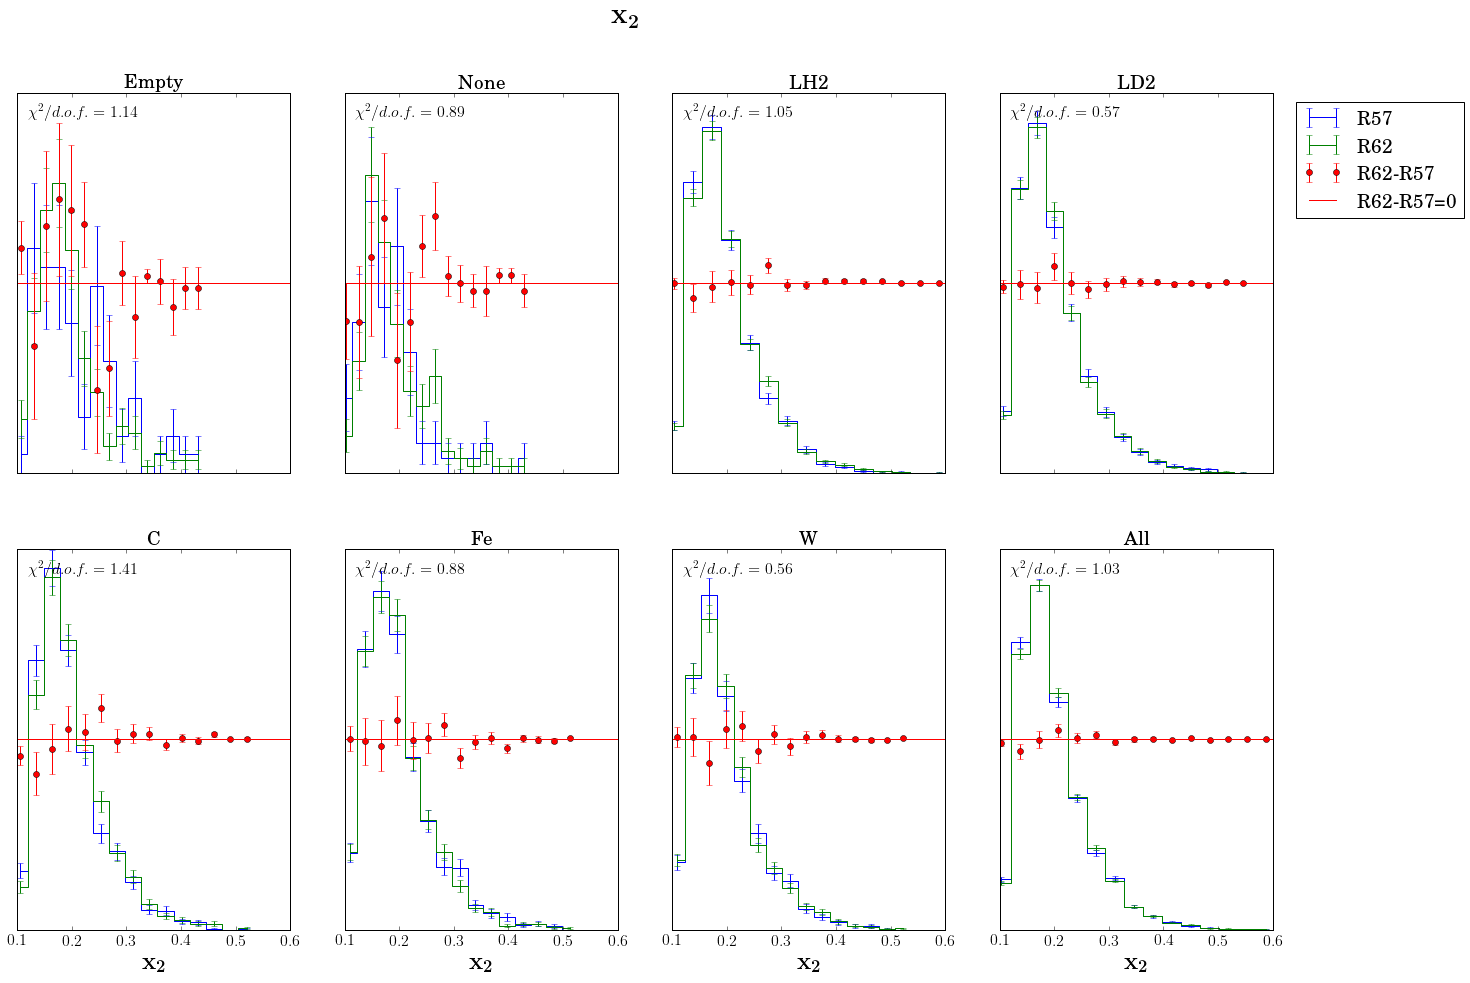
\includegraphics[width=0.6\textwidth]{figures/analysis/R57_R62_compare_xT.png}\vspace{5pt} \\
	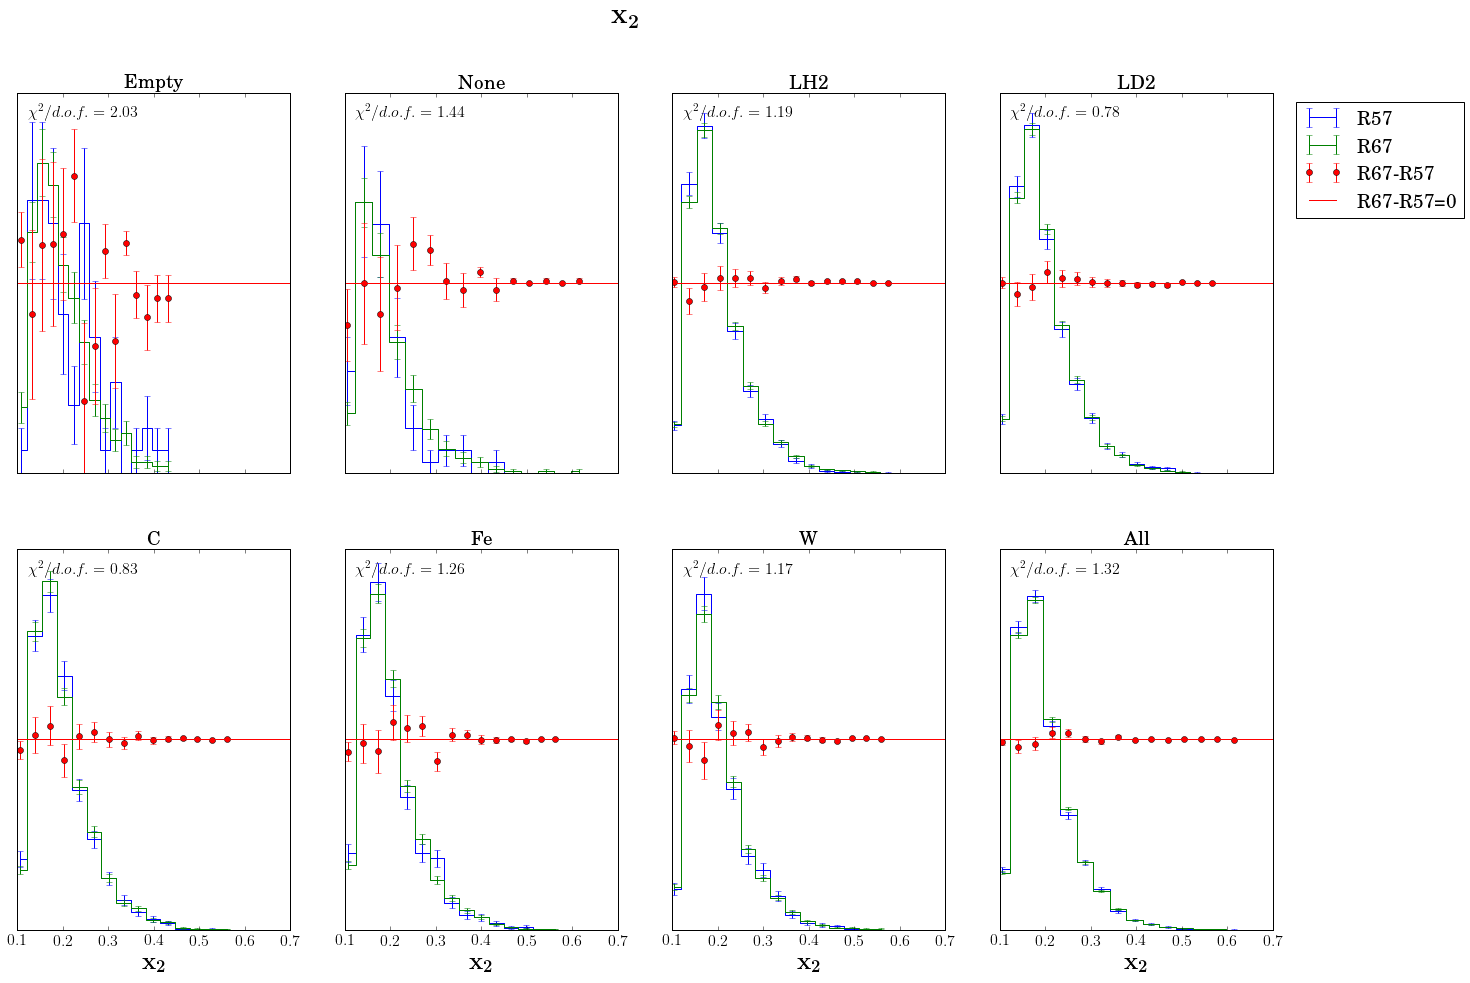
\includegraphics[width=0.6\textwidth]{figures/analysis/R57_R67_compare_xT.png} \vspace{5pt} \\
	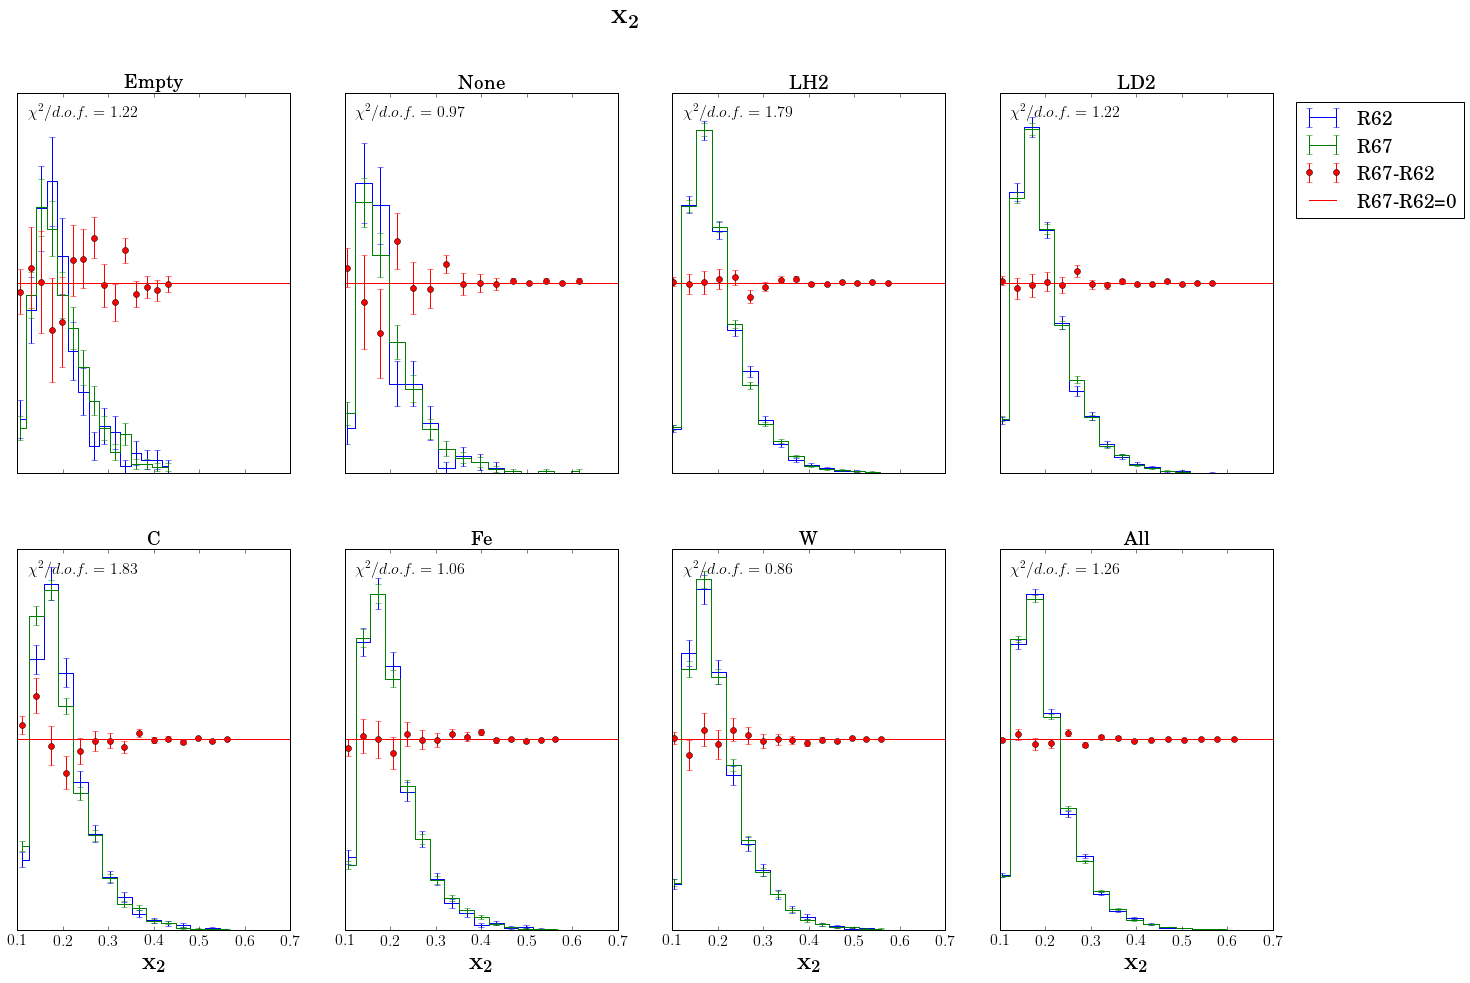
\includegraphics[width=0.6\textwidth]{figures/analysis/R62_R67_compare_xT.png}
	\caption{A comparison of $x_2$ distributions between roadsets for each target, and all targets combined. The difference between the two normalized distributions shown by the red data points, with a red line at zero. The $\chi^2$ shown is for the comparison between the roadset differences and the line at zero.}
	\label{fig:roadset-x2-compare}
\end{figure}

\begin{figure}
	\centering
	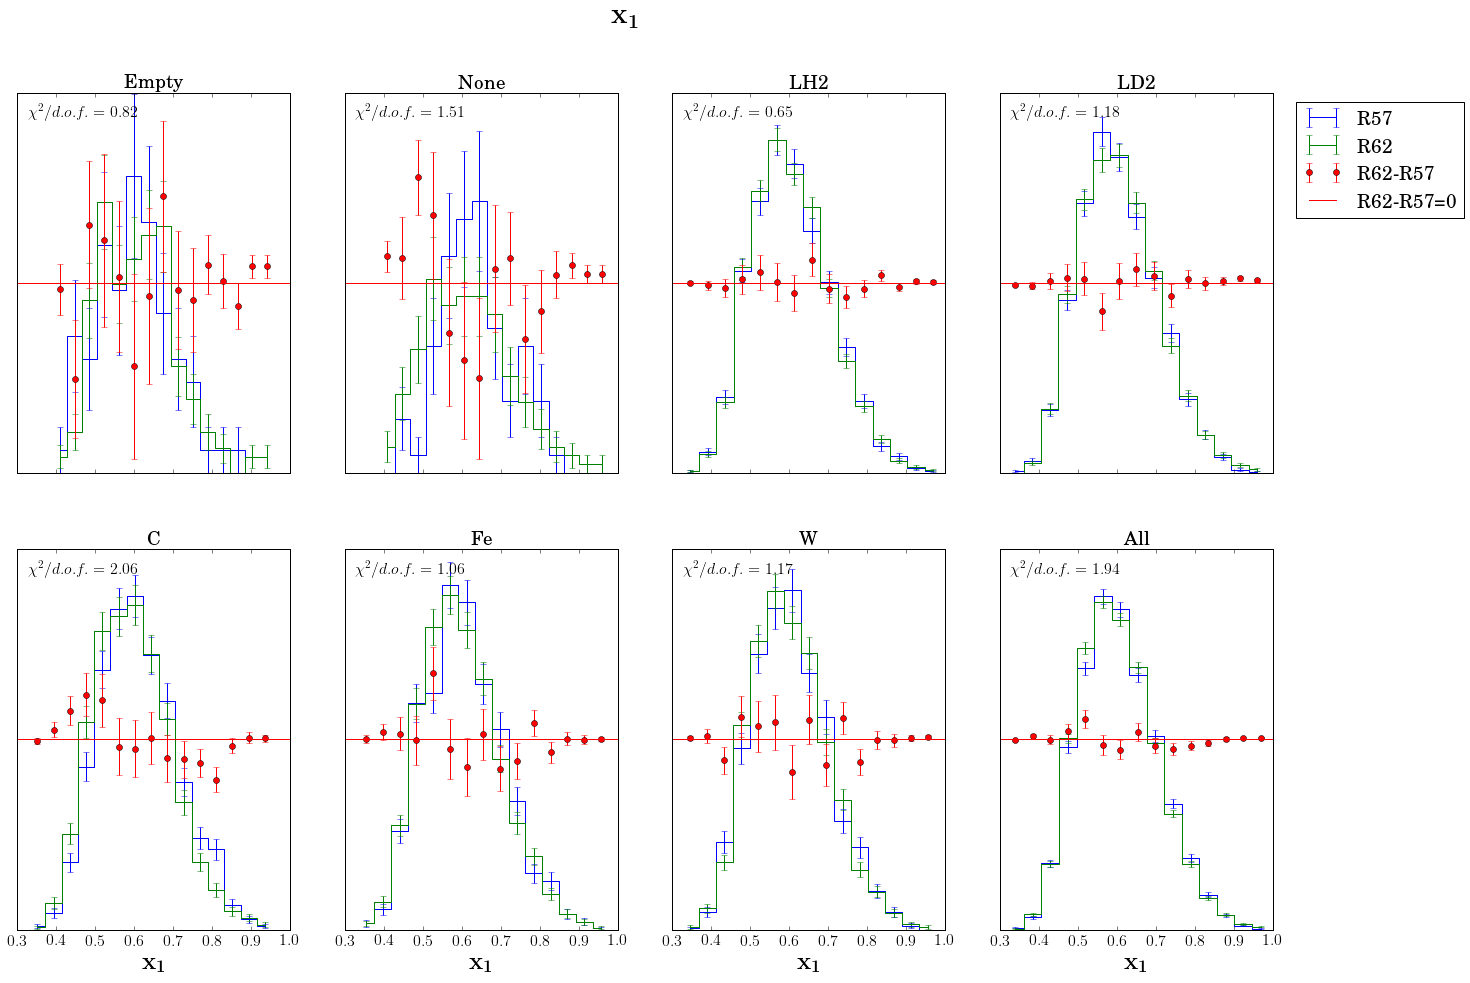
\includegraphics[width=0.6\textwidth]{figures/analysis/R57_R62_compare_xB.png}\vspace{5pt} \\
	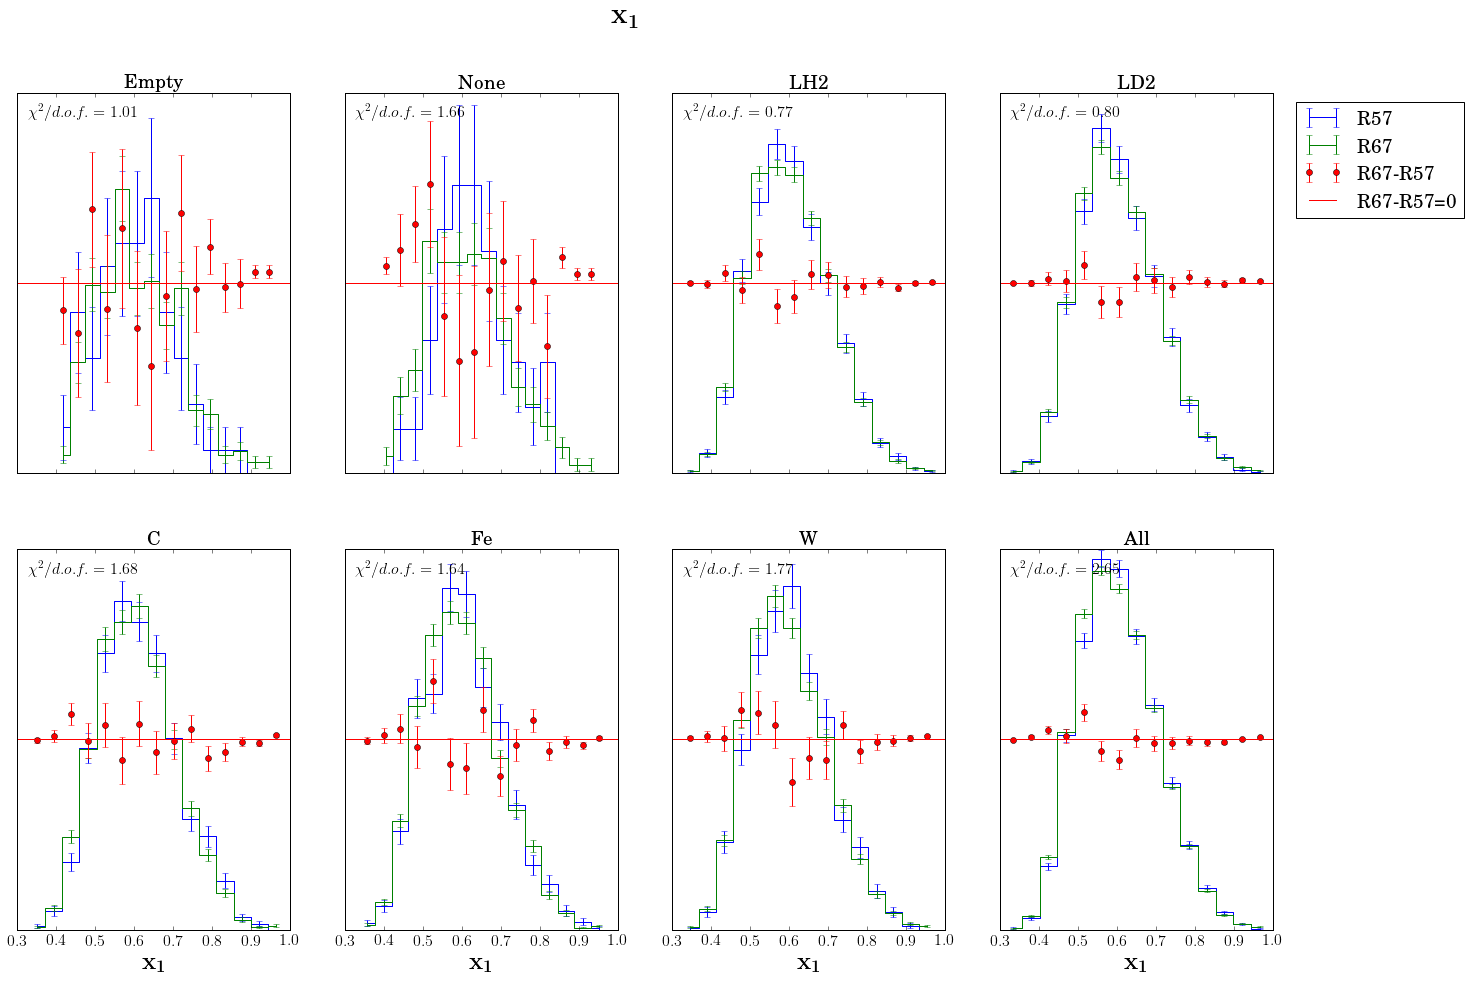
\includegraphics[width=0.6\textwidth]{figures/analysis/R57_R67_compare_xB.png} \vspace{5pt} \\
	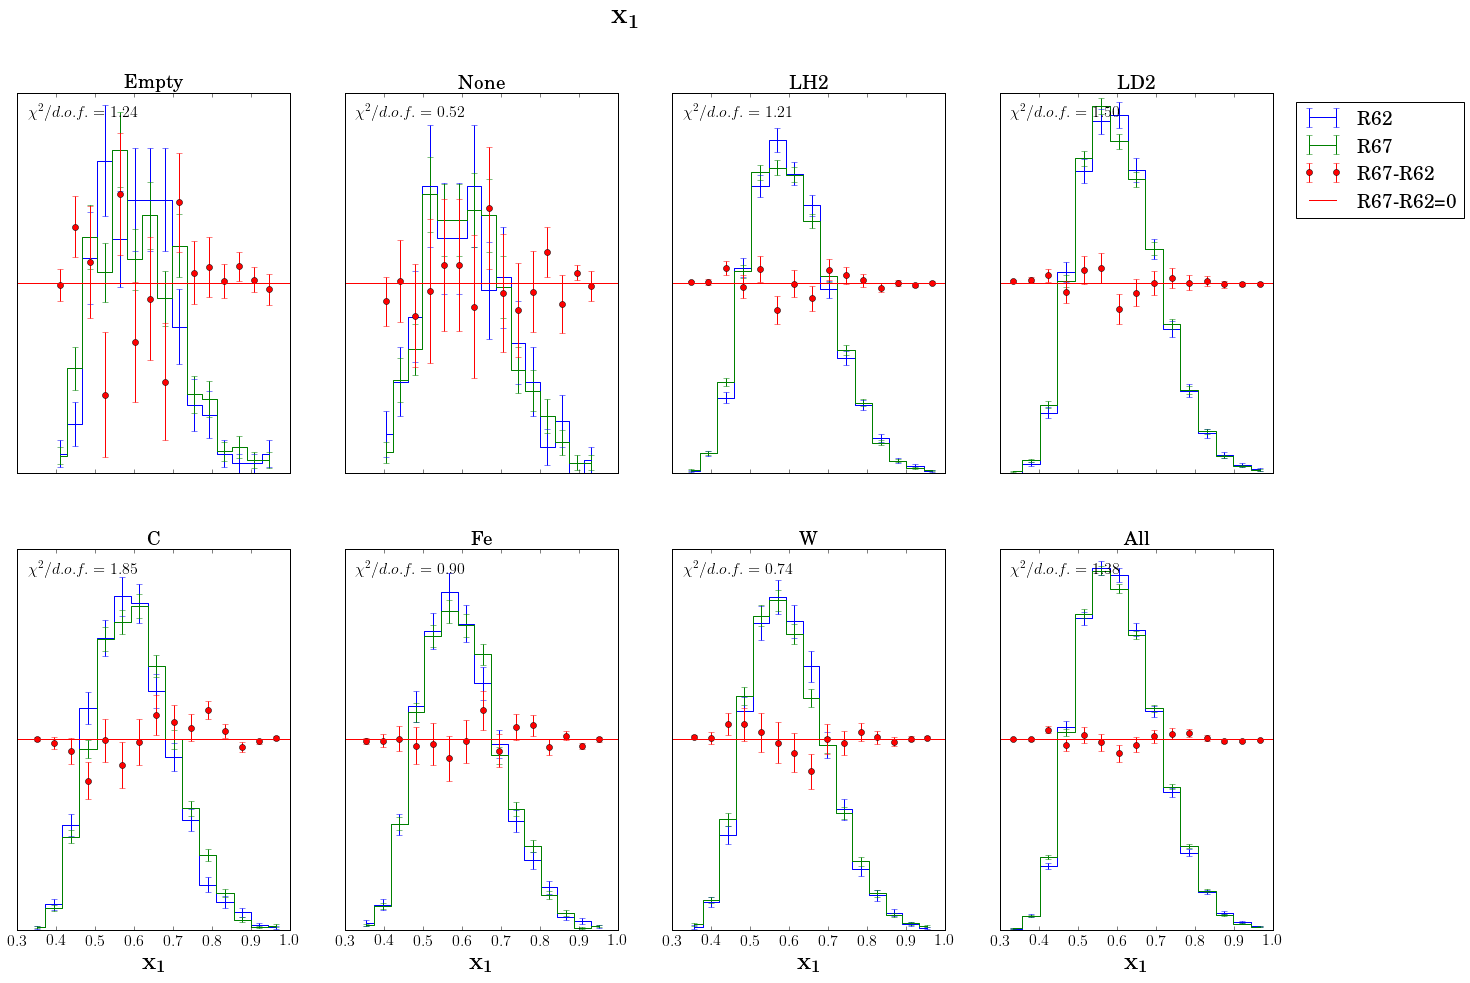
\includegraphics[width=0.6\textwidth]{figures/analysis/R62_R67_compare_xB.png}
	\caption{A comparison of $x_1$ distributions between roadsets for each target, and all targets combined. The difference between the two normalized distributions shown by the red data points, with a red line at zero. The $\chi^2$ shown is for the comparison between the roadset differences and the line at zero.}
	\label{fig:roadset-x1-compare}
\end{figure}

\begin{figure}
	\centering
	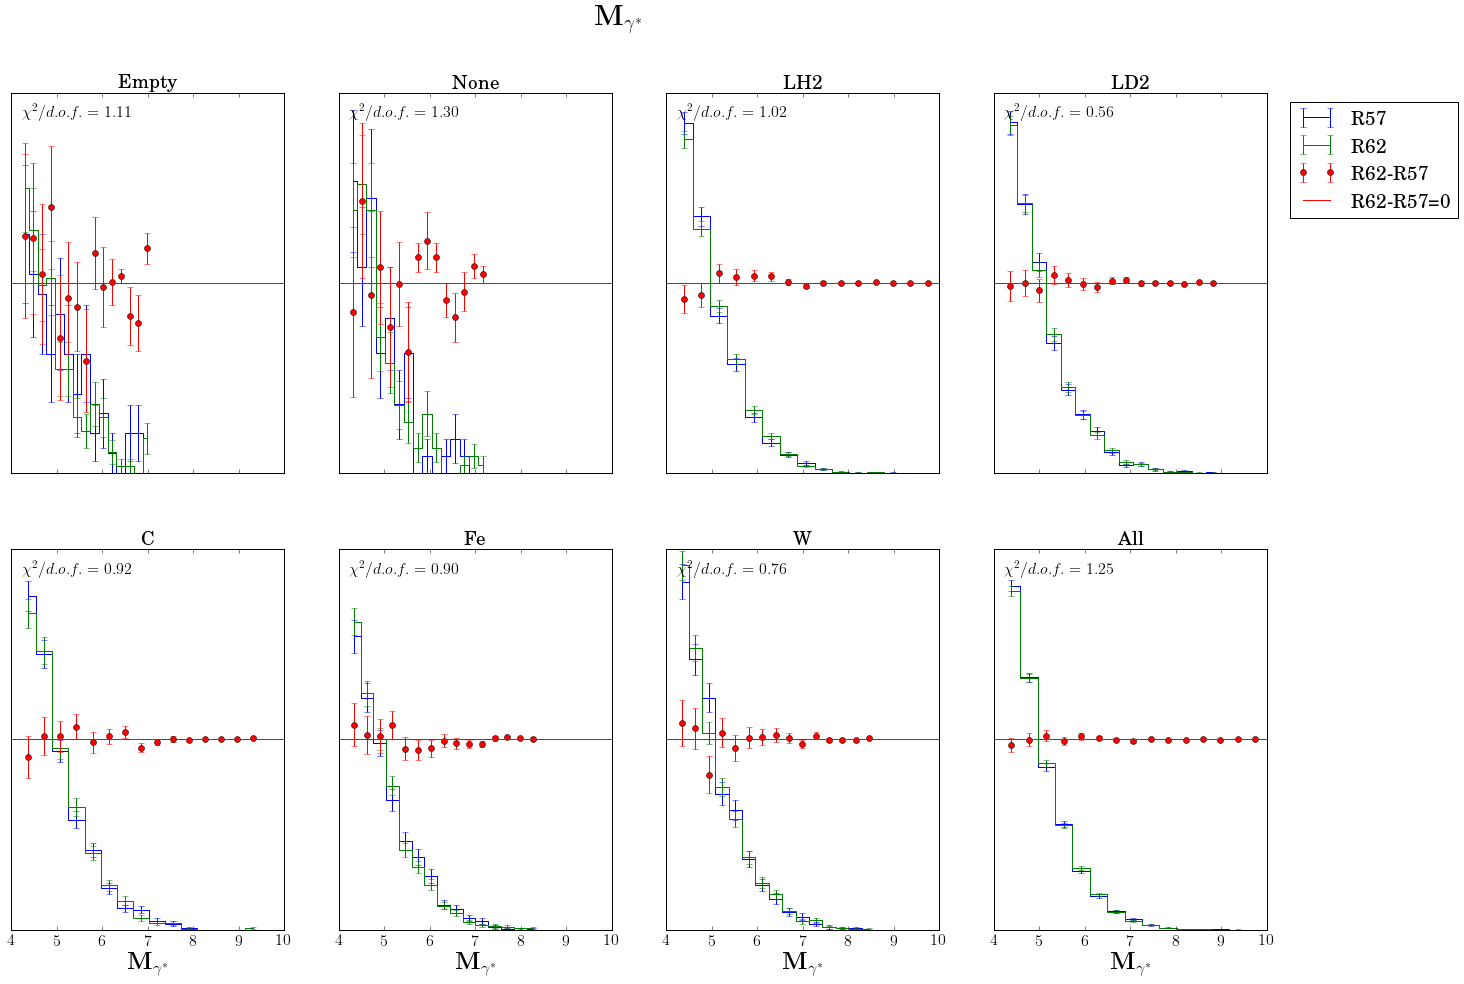
\includegraphics[width=0.6\textwidth]{figures/analysis/R57_R62_compare_mass.png}\vspace{5pt} \\
	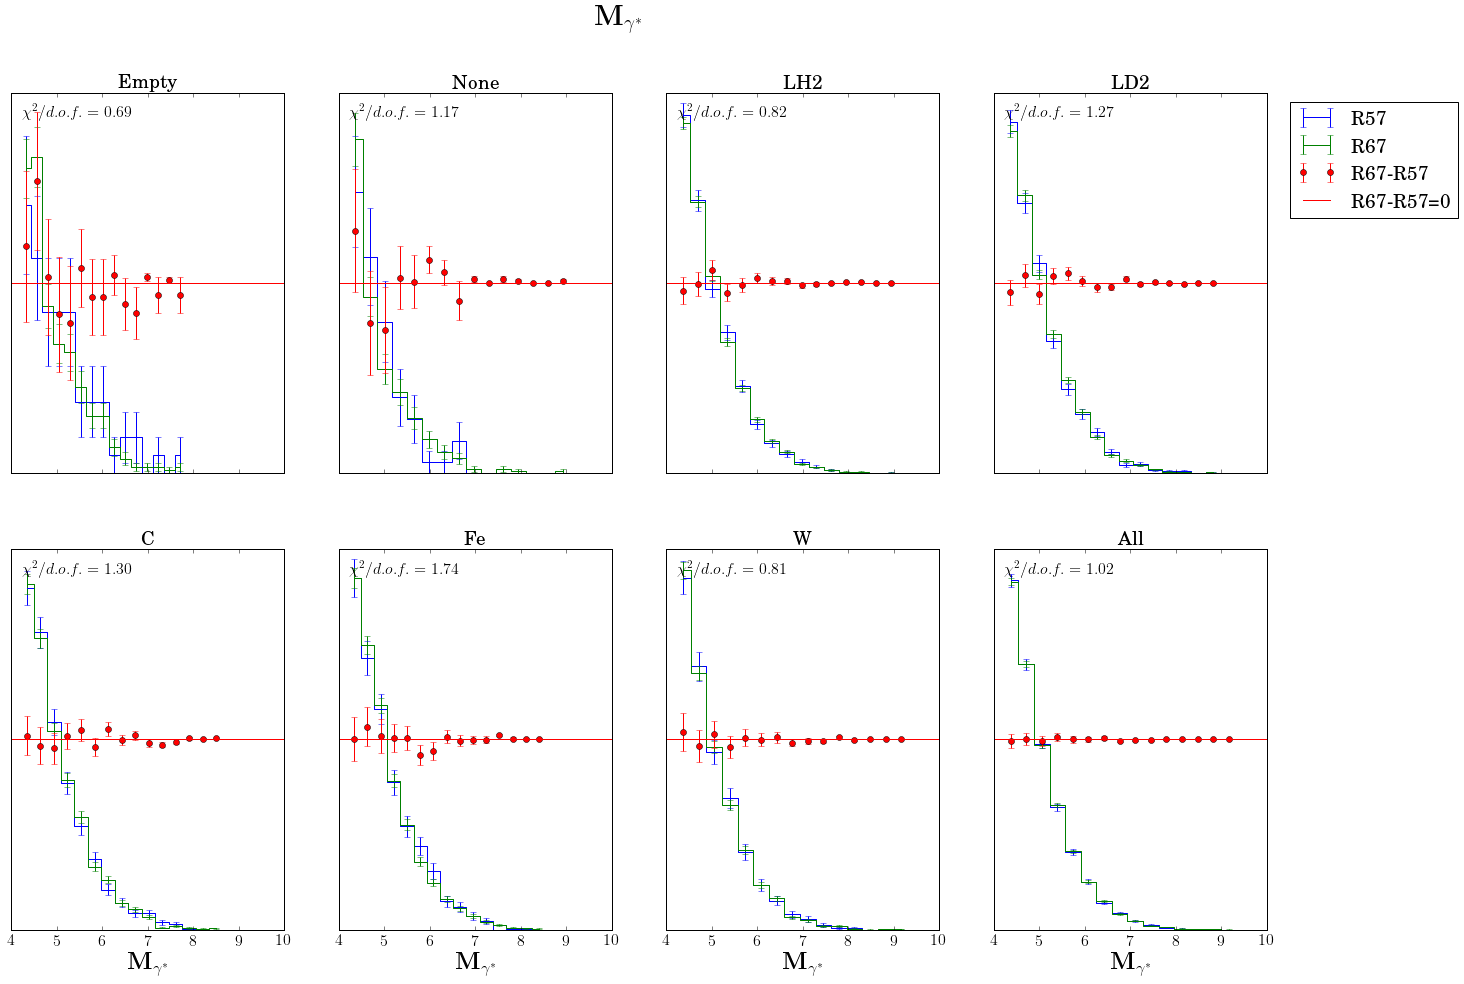
\includegraphics[width=0.6\textwidth]{figures/analysis/R57_R67_compare_mass.png} \vspace{5pt} \\
	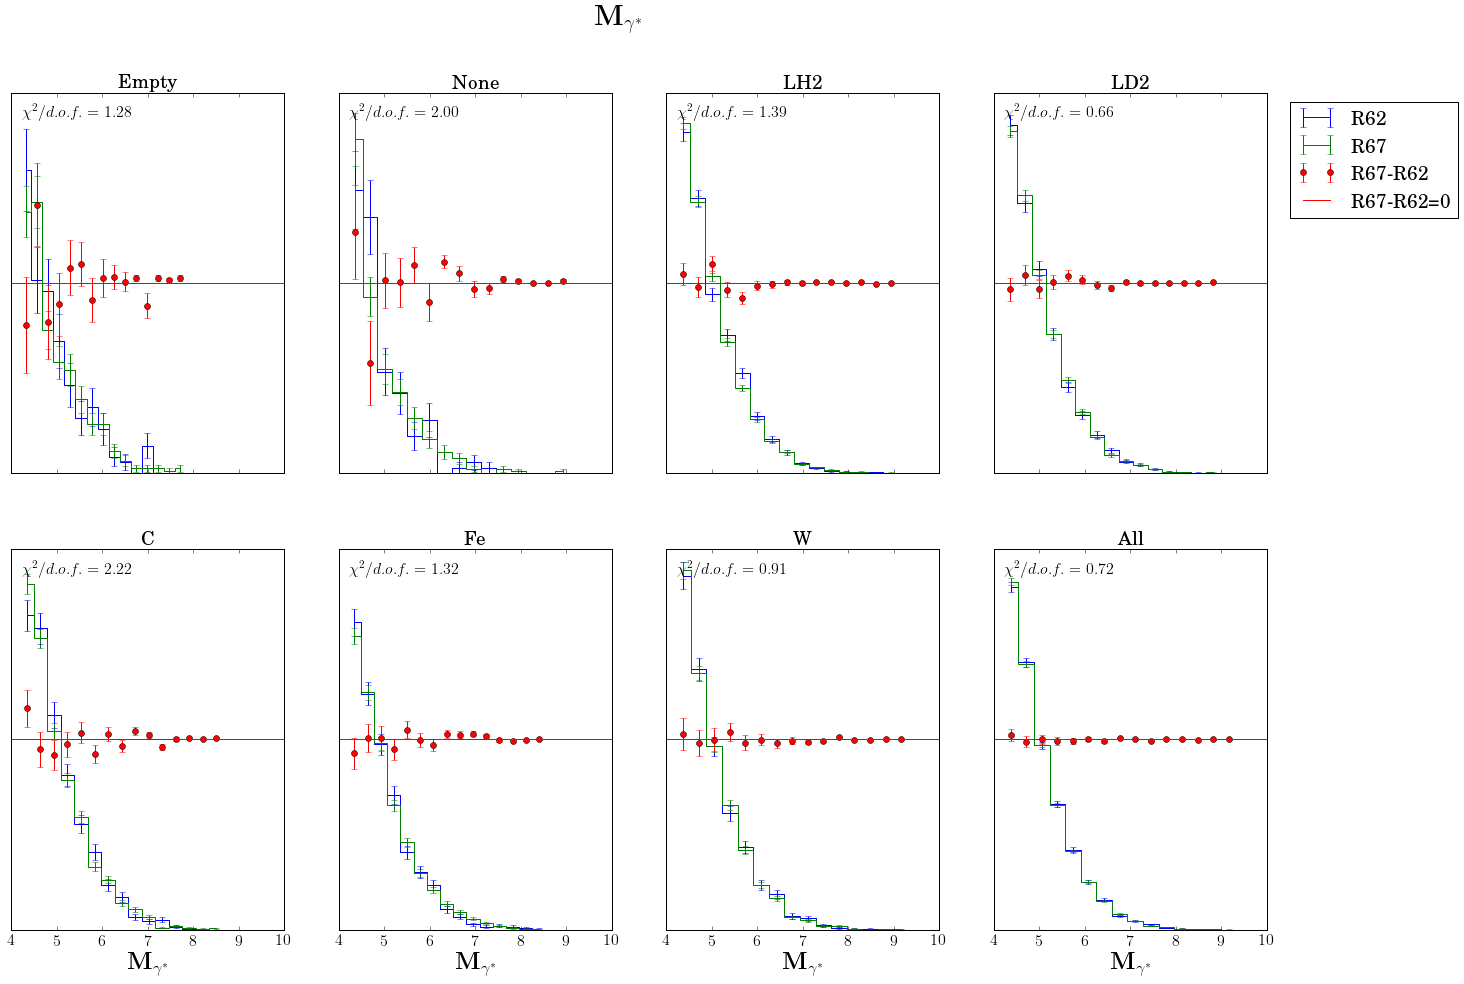
\includegraphics[width=0.6\textwidth]{figures/analysis/R62_R67_compare_mass.png}
	\caption{A comparison of $M_{\gamma^*}$ distributions between roadsets for each target, and all targets combined. The difference between the two normalized distributions shown by the red data points, with a red line at zero. The $\chi^2$ shown is for the comparison between the roadset differences and the line at zero.}
	\label{fig:roadset-mass-compare}
\end{figure}

\begin{figure}
	\centering
	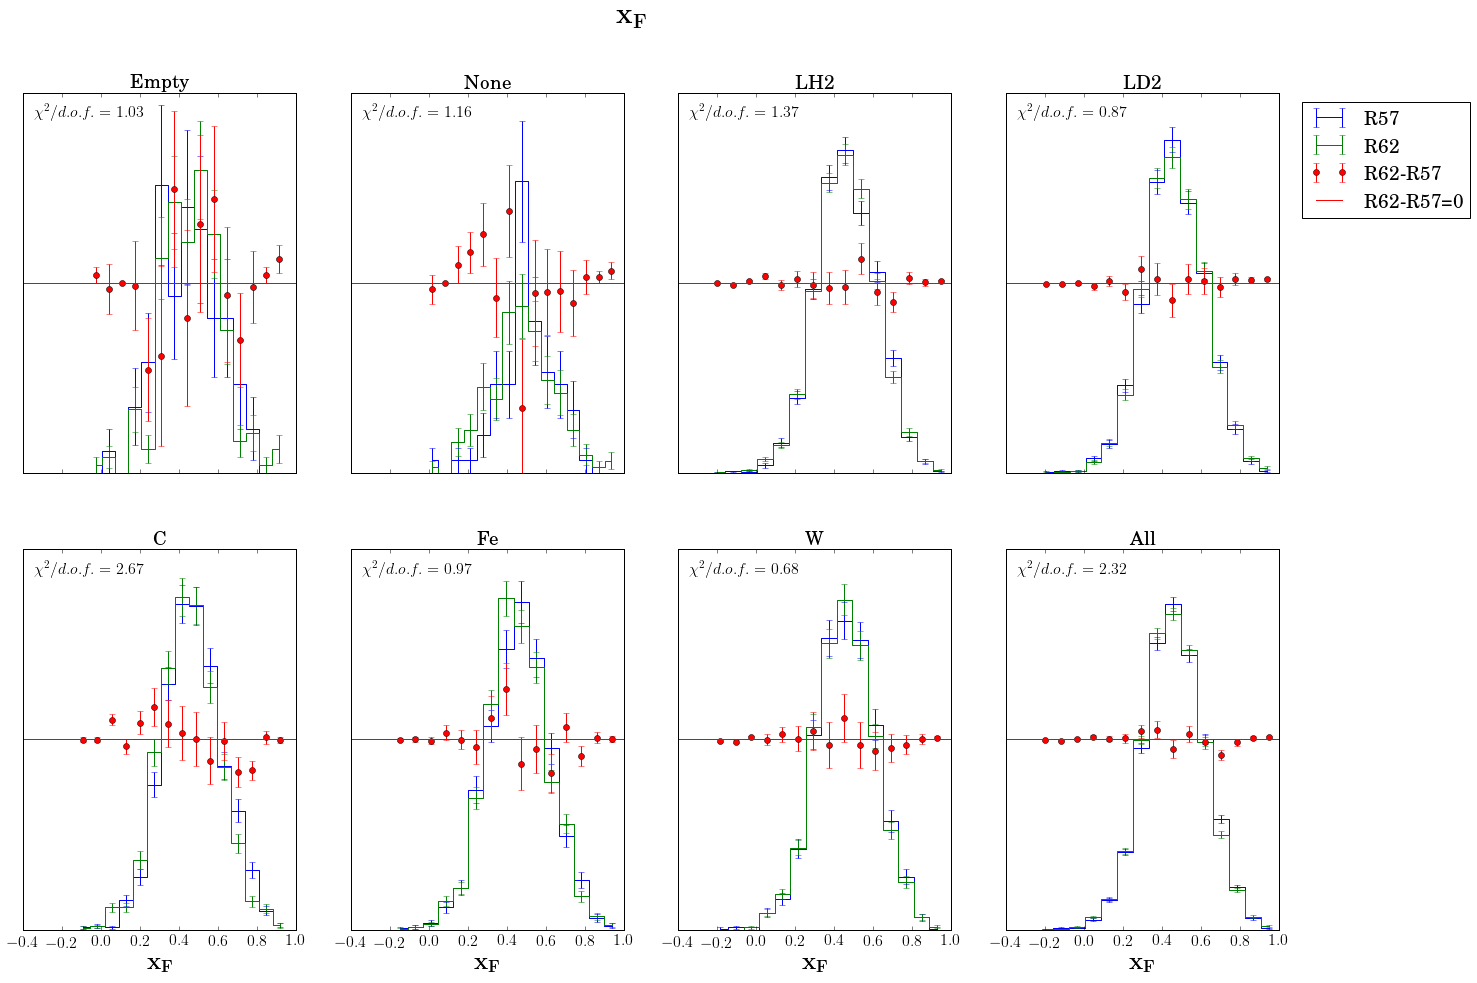
\includegraphics[width=0.6\textwidth]{figures/analysis/R57_R62_compare_xF.png}\vspace{5pt} \\
	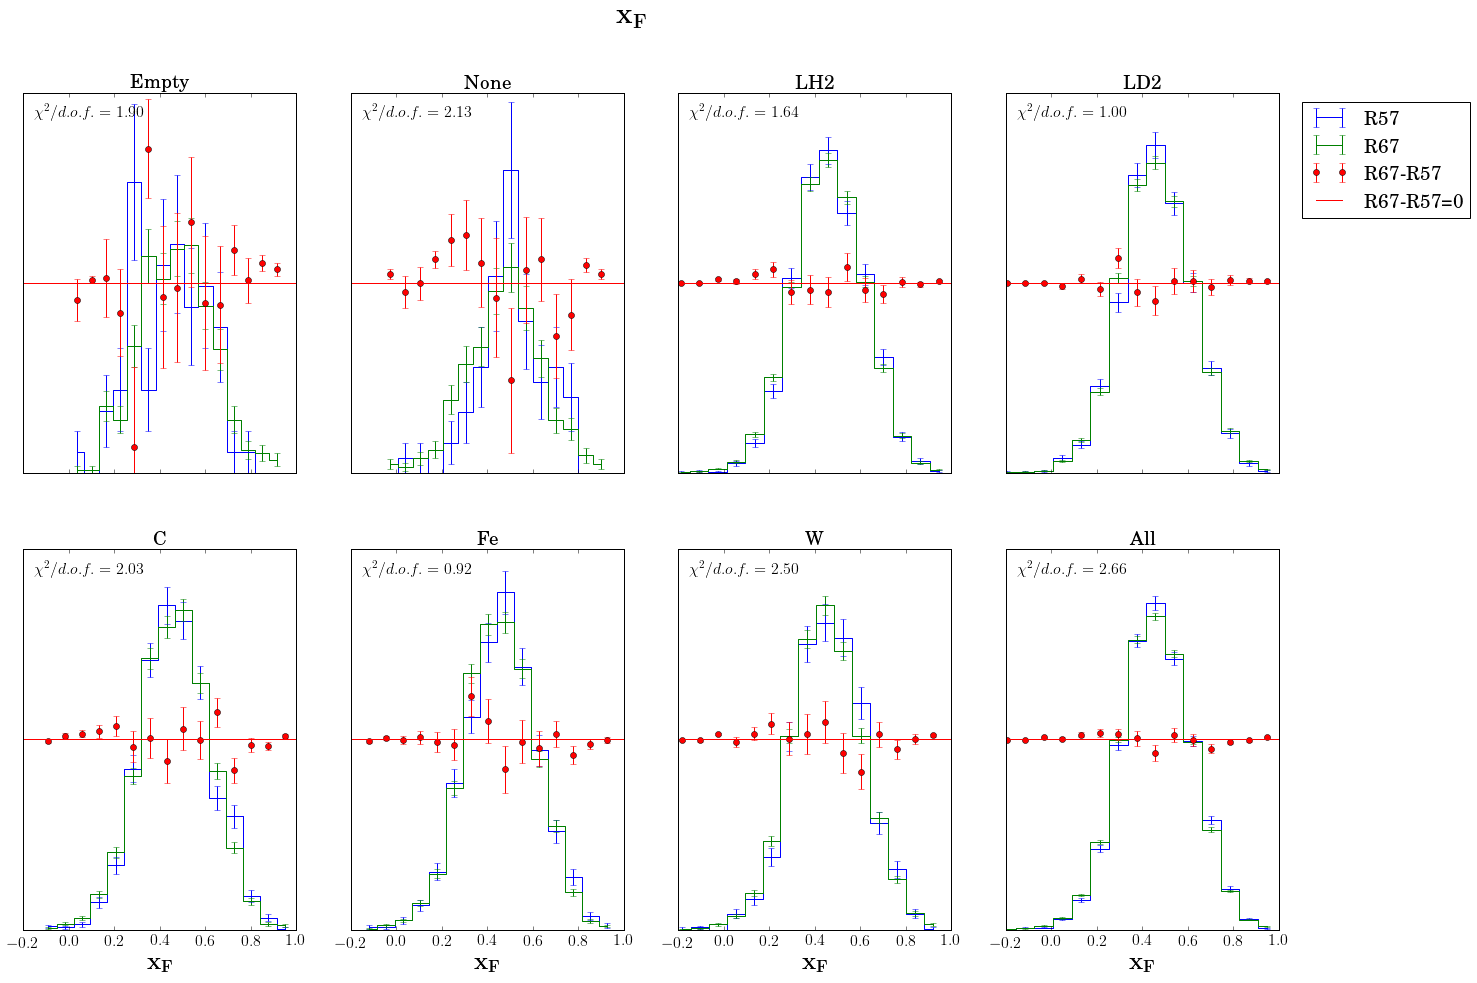
\includegraphics[width=0.6\textwidth]{figures/analysis/R57_R67_compare_xF.png} \vspace{5pt} \\
	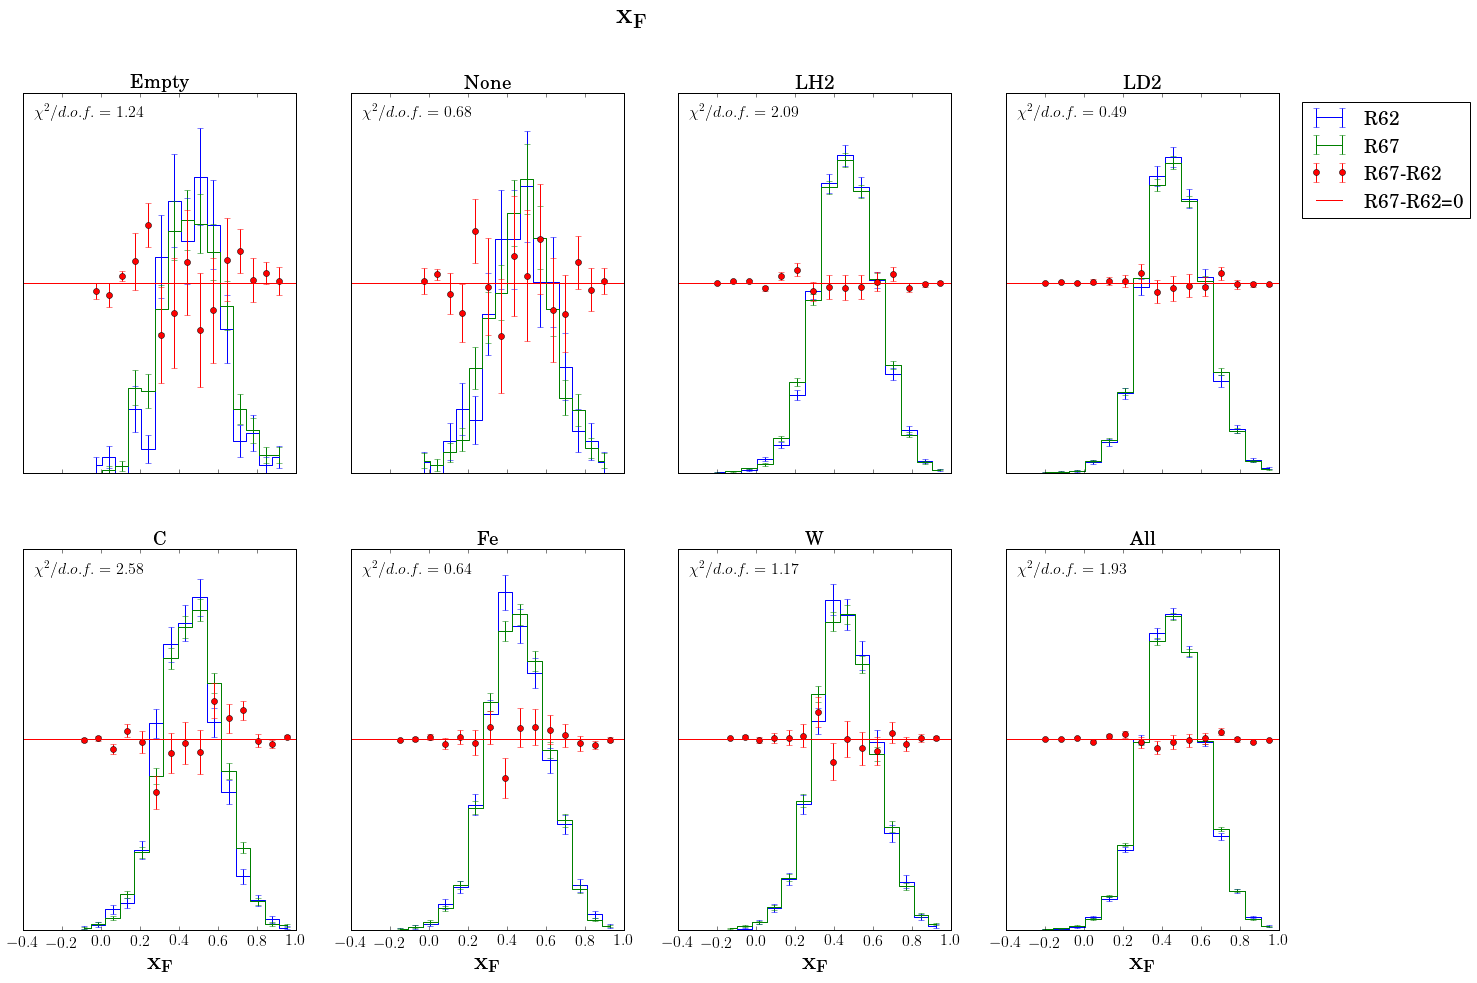
\includegraphics[width=0.6\textwidth]{figures/analysis/R62_R67_compare_xF.png}
	\caption{A comparison of $x_F$ distributions between roadsets for each target, and all targets combined. The difference between the two normalized distributions shown by the red data points, with a red line at zero. The $\chi^2$ shown is for the comparison between the roadset differences and the line at zero.}
	\label{fig:roadset-xF-compare}
\end{figure}